\documentclass[12pt,a4paper,titlepage]{article}
% Daniel Wong September 10, 2020

\usepackage[fleqn]{amsmath} % To write aligned equations
\usepackage{amssymb} % To write math symbols
\usepackage{graphicx,float} % To add pictures
\usepackage{caption} % To add captions
\usepackage{subcaption} % To add subcaptions
\usepackage{multirow} % To add multirow lines in tables
\usepackage{multicol} % To add multicolumn lines in tables
\usepackage{hyperref} % To add hyperlinks
\usepackage[normalem]{ulem} % To underline
\usepackage[backend=bibtex,citestyle=numeric,autocite=plain,sorting=none]{biblatex} % To add references
\usepackage[english]{babel} % To write accented vowels
\usepackage[toc,page]{appendix} % To add table of contents
\usepackage{physics} % To use supported physics notation
\usepackage[none]{hyphenat} % To remove hyphenation
\usepackage{mathtools}  % To use \mathclap which removes white space for subscripts
\usepackage{tensor} % For subscripts to the left

\usepackage{fancyhdr} % To input custom headers
\pagestyle{fancy} % Defines header for all pages other than plain-style pages
\fancyhf{}
\rhead{\nouppercase\leftmark}
\lfoot{Daniel Wong}
\rfoot{\thepage}
\renewcommand{\headrulewidth}{0.4pt} % Defining width of header line
\renewcommand{\footrulewidth}{0.4pt} % Defining width of footer line

\usepackage{tikz} % To input mathematical plots and diagrams
\usetikzlibrary{decorations.pathreplacing,decorations.pathmorphing,decorations.markings} % For curly braces, wavy lines, and arrow markings
\usetikzlibrary{tikzmark} % For adding annotations to equations
\usetikzlibrary{shapes.geometric} % For drawing regular polygons
\usetikzlibrary{shapes.misc} % For drawing crosses
\usetikzlibrary{snakes} % For drawing zigzag lines

\tikzset{->-/.style={decoration={markings,mark=at position #1 with {\arrow{>}}},postaction={decorate}}} 
\tikzset{-<-/.style={decoration={markings,mark=at position #1 with {\arrow{<}}},postaction={decorate}}} % Defining lines with arrows in the middle
\tikzset{cross/.style={cross out,draw,minimum size=2*(#1-\pgflinewidth),inner sep=0pt,outer sep=0pt}} % Defining cross for a node

\usepackage{color} % To use different colours
\usepackage[makeroom]{cancel} % To cancel terms in equations

\definecolor{lightGray}{gray}{0.8}

\newcommand{\trm}[1]{\textrm{#1}} % Shorthand for \textrm command
\newcommand{\up}{\uparrow} % Shorthand for \uparrow command
\newcommand{\dn}{\downarrow} % Shorthand for \downarrow command
\newcommand{\en}{\epsilon_{0}} % Shorthand for \epsilon_{0}
\newcommand{\ul}[1]{\underline{\smash{#1}}} % Properly underlines words
\newcommand{\explain}[1]{% Adds an arrow to allow for explanations in equations
	\quad\rotatebox[origin=c]{180}{\enskip$\Lsh$}\hfill
	\begin{minipage}[t]{\dimexpr\linewidth-8em\relax}
	#1
	\end{minipage}\hspace{4em}\bigskip
}

\newcommand{\aside}[1]{% Aligns the environment for asides
	\ul{Aside}:\hfill
	\begin{minipage}[t]{\dimexpr\linewidth-8em\relax}
	#1
	\end{minipage}\hspace{4em}\bigskip
}

\newcommand{\theorem}[1]{% Aligns the environment for theorems
	\ul{Theorem}:\hfill
	\begin{minipage}[t]{\dimexpr\linewidth-8em\relax}
	#1
	\end{minipage}\hspace{4em}\bigskip
}

\newcommand{\proof}[1]{% Aligns the environment for theorems
	\ul{Proof}:\hfill
	\begin{minipage}[t]{\dimexpr\linewidth-8em\relax}
	#1
	\end{minipage}\hspace{4em}\bigskip
}

\newcommand{\definition}[1]{% Aligns the environment for definitions
	\ul{Definition}:\hfill
	\begin{minipage}[t]{\dimexpr\linewidth-8em\relax}
	#1
	\end{minipage}\hspace{4em}\bigskip
}
\newcommand{\example}[2]{% Aligns the environment for examples
	\bigskip
	\hrule
	\bigskip
	\ul{Ex #1}:\hfill
	\begin{minipage}[t]{\dimexpr\linewidth-8em\relax}
	#2
	\end{minipage}\hspace{4em}
	\bigskip
	\hrule
	\bigskip
}

\newcommand{\angstrom}{\textup{\AA}} % Angstrom symbol
\newcommand{\Chi}{\mathcal{X}} % Inline chi symbol
\newcommand{\Tau}{\mathcal{T}} % Capital tau symbol
\newcommand{\sign}{\trm{sign}} % Sign function
\newcommand{\pd}[1]{\partial_{#1}} % Covariant 4-gradient
\newcommand{\pu}[1]{\partial^{#1}} % Contravariant 4-gradient
\newcommand{\id}{\mathbb{I}} % Identity matrix
\renewcommand{\Re}{\trm{Re}} % Real
\renewcommand{\Im}{\trm{Im}} % Imaginary
\renewcommand{\CancelColor}{\color{red}} % Changes the cancel colour to red

\begin{document}
\title{PHYS 434: Quantum Physics III}
\author{Daniel Wong\\University of Waterloo\\Instructor: Dr. Anton Burkov}
\date{Fall 2017}
\maketitle

\setlength\parindent{0pt}
\pagenumbering{roman}
\numberwithin{equation}{section}

\section*{Disclaimer}
These notes may be freely used by anyone who comes across them. If any errors are found within these notes, please email me at \ul{temp@temp.com}. If you are the previous instructor of this course (Dr. Anton Burkov) and have concerns about keeping these notes on my website, please contact me at the email provided.\\

Other course notes may be found on my website at \url{www.temp.com/notes}.

\newpage
\tableofcontents
\newpage
\pagenumbering{arabic}

\section{Review of Quantum Mechanics}
\subsection{Discrete Spectrum}
States of the system in quantum mechanics are vectors in Hilbert space $\mathcal{H}$. The Hilbert space $\mathcal{H}$ is the space of all states of a given system. In Dirac notation, the states are called kets $\ket{\psi}$.\\

Observables in quantum mechanics are operators $\vb{A}:\mathcal{H}\rightarrow\mathcal{H}$ acting on kets such that $\vb{A}\ket{\psi}=\ket{\varphi}$. Every operator $\vb{A}$ has a set of eigenstates (or eigenkets) $\{\ket*{a'}\}$ where
\begin{equation}
\begin{aligned}
\vb{A}\ket*{a'}&=a'\ket*{a'}\\
\vb{A}\ket*{a''}&=a''\ket*{a''}
\end{aligned}
\end{equation}
The eigenvalue corresponding to the eigenket $\ket*{a'}$ is denoted $a'\in\mathbb{R}$.\\

The dual Hilbert space to the ket space is the bra space. Elements of the bra space are bras and are denoted as $\bra{\varphi}$.\\

One can now define an inner product (or scalar product) of a bra $\bra{\varphi}$ and ket $\ket{\psi}$ to be $\braket{\varphi}{\psi}$. By definition
\begin{equation}
\braket{\varphi}{\psi}=\braket{\psi}{\varphi}^{*}
\end{equation}
This implies that $\braket{\psi}{\psi}=\braket{\psi}{\psi}^{*}$ is real. We postulate that $\braket{\psi}{\psi}$ is non-negative, meaning
\begin{equation}
\norm{\psi}=\braket{\psi}{\psi}^{\frac{1}{2}}\geq0
\end{equation}

Thus, every state in the Hilbert space can be normalized.
\begin{equation}
\begin{aligned}
\ket*{\widetilde{\psi}}&=\frac{1}{\sqrt{\braket{\psi}{\psi}}}\ket{\psi}\\
\implies \braket*{\widetilde{\psi}}{\widetilde{\psi}}&=\frac{\braket{\psi}{\psi}}{\braket{\psi}{\psi}}=1
\end{aligned}
\end{equation}
If one has that $\braket{\varphi}{\psi}=0$, then $\ket{\psi}$ and $\ket{\varphi}$ are orthogonal.\\

The dual of $\vb{A}\ket{\psi}$ is $\bra{\psi}\vb{A}^{\dagger}$, where $\vb{A}^{\dagger}$ is the Hermitian adjoint of $\vb{A}$. One can act on the ket $\vb{A}\ket{\psi}$ with the bra $\bra{\varphi}$ and obtain
\begin{equation}
\mel{\varphi}{\vb{A}}{\psi}=\mel{\psi}{\vb{A}^{\dagger}}{\varphi}^{*}
\end{equation}

The operator is Hermitian if $\vb{A}^{\dagger}=\vb{A}$. For $\vb{A}$ as a Hermitian operator, let $(a',\ket*{a'})$ and $(a'',\ket*{a''})$ be two eigenpairs. Thus
\begin{equation}
\begin{aligned}
\vb{A}\ket*{a'}&=a'\ket*{a'}\\
\vb{A}\ket*{a''}&=a''\ket*{a''}
\end{aligned}
\end{equation}

Let $\bra{\varphi}$ be an arbitrary bra. Thus
\begin{equation}
\begin{aligned}
\mel*{\varphi}{\vb{A}}{a''}&=\mel*{\varphi}{a''}{a''}=a''\braket*{\varphi}{a''}\\
\mel*{a''}{\vb{A}}{\varphi}&=\mel*{\varphi}{\vb{A}}{a''}^{*}=a''^{*}\braket*{a''}{\varphi}
\end{aligned}
\end{equation}
Since $\bra{\varphi}$ is arbitrary
\begin{equation}
\bra*{a''}\vb{A}=a''^{*}\bra*{a''}
\end{equation}
From $\vb{A}\ket*{a'}=a'\ket*{a'}$ and $\bra*{a''}\vb{A}=a''^{*}\bra*{a''}$
\begin{equation}
\begin{aligned}
\mel*{a''}{\vb{A}}{a'}=a'\braket*{a''}{a'}=a''^{*}\braket*{a''}{a'}\\
\implies (a'-a''^{*})\braket*{a''}{a'}=0
\end{aligned}
\end{equation}
One can choose $\ket*{a''}=\ket*{a'}$ to show
\begin{equation}
(a'-a'^{*})\braket*{a'}{a'}=0 \implies a'=a'^{*}
\end{equation}
since $\braket*{a'}{a'}>0$ with $\ket*{a'}\neq\ket{0}$. Thus, all Hermitian operators have real eigenvalues. Since the spectrum of an operator correspond to physical observales, this is in agreement with the fact that all physical quantities are real-valued.\\

Consider now $\ket*{a'}$ and $\ket*{a''}$ to be different and non-degenerate (different eigenvalues). Thus
\begin{equation}
\begin{aligned}
(a'-a''^{*})\braket*{a''}{a'}&=0\\
(a'-a'')\braket*{a''}{a'}&=0\trm{, since all eigenvalues are real}\\
\braket*{a''}{a'}&=0\trm{, since $\ket*{a'}$ and $\ket*{a''}$ are non-degenerate}
\end{aligned}
\end{equation}
Thus, eigenstates corresponding to different eigenvalues are orthogonal. We shall also assert all eigenstates are normalized, since their norm is arbitrary. Thus, these results can be represented as 
\begin{equation}
\braket*{a'}{a''}=\delta_{a'a''}
\end{equation}

Thus, the set of eigenkets of any Hermitian operator forms a complete orthonormal set of states and act as a basis for the Hilbert space. Thus, any ket $\ket{\psi}$ can be written as a linear combination of eigenkets for any Hermitian operator $\vb{A}$.
\begin{equation}
\ket{\psi}=\sum_{a'}c_{a'}\ket{a'}
\end{equation}
Using the orthonormality of eigenkets
\begin{equation}
\begin{aligned}
\braket*{a''}{\psi}&=\sum_{a'}c_{a'}\braket*{a''}{a'}=\sum_{a'}c_{a'}\delta_{a''a'}=c_{a''}\\
\implies c_{a'}&=\braket*{a'}{\psi}\in\mathbb{C}
\end{aligned}
\end{equation}
Physically, $c_{a'}$ is the probability amplitude. For a sysem in state $\ket{\psi}$, the probability of measuring the value $a'$ when making measurement $\vb{A}$ is the square modulus of $c_{a'}$ (i.e. $\abs{c_{a'}}^{2}$). Equivalently, this is the same probability of finding state $\ket{\psi}$ in state $\ket*{a'}$ after measurement.\\

Writing $\ket{\psi}$ as a spectral decomposition gives
\begin{equation}
\ket{\psi}=\sum_{a'}\ket*{a'}\ip*{a'}{\psi}\trm{, since $c_{a'}=\ip*{a'}{\psi}$}
\end{equation}

Since $\ket{\psi}$ is arbitrary, one now obtains the closure relation (or resolution of identity).
\begin{equation}
\sum_{a'}\op*{a'}{a'}=\mathbb{I}
\end{equation}

An individual term in this sum is called the projection operator.
\begin{equation}
\begin{aligned}
\Lambda_{a'}&=\op*{a'}{a'}\\
\Lambda_{a'}\ket{\psi}&=\ket*{a'}\ip*{a'}{\psi}&=c_{a'}\ket{a'}
\end{aligned}
\end{equation}
As such, $\Lambda_{a'}$ projects $\ket{\psi}$ into the direction of eigenket $\ket{a'}$.\\

Using the closure relation, one can obtain the spectral decomposition of operator $\vb{A}$.
\begin{equation}
\vb{A}\op*{a'}{a'}=a'\op*{a'}{a'}
\end{equation}
Taking the sum over all eigenkets
\begin{equation}
\vb{A}\sum_{a'}\op*{a'}{a'}=\vb{A}\mathbb{I}=\vb{A}=\sum_{a'}\op*{a'}{a'}
\end{equation}

Consider another operator $\vb{B}$.
\begin{equation}
\vb{B}=\mathbb{I}\vb{B}\mathbb{I}=\sum_{a'a''}\op*{a''}{a''}\vb{B}\op*{a'}{a'}
\end{equation}
$\mel*{a''}{\vb{B}}{a'}$ can be interpreted as a matrix indexed by $\ket*{a''}$ and $\ket*{a'}$.

\begin{equation}
\vb{B}=\mqty(\mel*{a^{(1)}}{\vb{B}}{a^{(1)}} & \ldots & \mel*{a^{(1)}}{\vb{B}}{a^{(n)}} \\ \vdots & \ddots & \vdots \\ \mel*{a^{(n)}}{\vb{B}}{a^{(1)}} & \ldots & \mel*{a^{(n)}}{\vb{B}}{a^{(n)}})
\end{equation}
The matrix that corresponds to $\vb{B}^{\dagger}$ is the complex conjugate transposed of the matrix corresponding to $\vb{B}$.

\subsection{Continuous Spectrum}
Let us now generalize to operators with continuous spectrum. For example, the position and momentum operators are two such operators. Let $\ket*{x'}$ be a position eigenket corresponding to the state of a particle at position $x'$ in space. Let $\vb{x}$ be the position operator defined as
\begin{equation}
\vb{x}\ket*{x'}=x'\ket*{x'}
\end{equation}
Define $\psi(x')$ as the probability amplitude to find a particle in a state $\ket{\psi}$ at position $x'$. It is given by
\begin{equation}
\psi(x')=\ip*{x'}{\psi}
\end{equation}
This is equal to the wavefunction.\\

For the continuous spectra, instead of using sums, one uses integrals. Generalizing the Kronecker delta equation to the continuous spectra, one obtains the Dirac delta function $\delta(x)$
\begin{equation}
\ip*{x'}{x''}=\delta(x'-x'')
\end{equation}
where the Dirac delta is defined as
\begin{equation}
\int_{-\infty}^{\infty}\dd{x'}f(x')\delta(x')=f(0)
\end{equation}

\begin{tikzpicture}
	\draw[<->] (-2,0) -- (2,0) node[right] {$x$};
	\draw[->] (0,0) -- (0,2) node[above] {$y$};
	\draw[red,thick,fill opacity=0.2,text opacity=1] (-2,0) -- (0,0) -- (0,2) -- (0,0) -- (2,0);
	\node at (0.5,1.5) {$\delta(x)$};
\end{tikzpicture}

The closure relation then becomes
\begin{equation}
\mathbb{I}=\int_{-\infty}^{\infty}\dd{x'}\op*{x'}{x'}
\end{equation}
Thus
\begin{equation}
\ket{\psi}=\mathbb{I}\ket{\psi}=\int\dd{x'}\ket*{x'}\ip*{x'}{\psi}
\end{equation}

Let $\ket{\varphi}$ be another ket in the same Hilbert space as $\ket{\psi}$.
\begin{equation}
\begin{aligned}
\ip{\varphi}{\psi}&=\int_{-\infty}^{\infty}\dd{x'}\ip*{\varphi}{x'}\ip*{x'}{\psi}\\
&=\int_{-\infty}^{\infty}\dd{x'}\ip*{x'}{\varphi}^{*}\ip*{x'}{\psi}\\
&=\int_{-\infty}^{\infty}\dd{x'}\varphi(x')^{*}\psi(x')
\end{aligned}
\end{equation}
Compare this to $\ip{\varphi}{\psi}=\sum_{a'}\ip*{\varphi}{a'}\ip*{a'}{\psi}$ in the discrete case.

\subsection{Infinitesimal Translations}
Introduce the infinitesimal translation operator $\vb{T}$ as
\begin{equation}
\vb{T}(\dd{x'})\ket*{\vec{x}\,'}=\ket*{\vec{x}\,'+\dd{\vec{x}\,'}}
\end{equation}
where $\dd{\vec{x}\,'}$ is an infinitesimally small vector. Acting on an arbitrary $\ket{\psi}$ state
\begin{equation}
\begin{aligned}
\vb{T}(\dd{\vec{x}\,'})\ket{\psi}&=\vb{T}(\dd{\vec{x}\,'})\underbrace{\int_{\mathbb{R}}\dd[3]{x'}\op*{\vec{x}\,'}{\vec{x}\,'}}_{\mathbb{I}}\ket*{\psi}\qq{(Note that $\dd{\vec{x}\,'}\neq\dd[3]x'$)}\\
&=\int_{\mathbb{R}}\dd[3]{x'}\ket*{\vec{x}\,'+\dd{\vec{x}\,'}}\ip*{\vec{x}\,'}{\psi}\\
&=\int_{\mathbb{R}}\dd[3]{x''}\ket*{\vec{x}\,''}\ip*{\vec{x}\,''-\dd{\vec{x}\,'}}{\psi},\qq{$\vec{x}\,''=\vec{x}\,'-\dd{\vec{x}\,'}$}
\end{aligned}
\end{equation}

Without loss of generality, let $\ket{\psi}$ be normalized (i.e. $\ip{\psi}{\psi}=1$). It is useful to define $\vb{T}(\dd{\vec{x}\,'})$ such that $\vb{T}(\dd{\vec{x}\,'})\ket{\psi}$ is also normalized. Thus
\begin{equation}
\mel*{\psi}{\vb{T}^{\dagger}(\dd{\vec{x}\,'})\vb{T}(\dd{\vec{x}\,'})}{\psi}=1
\end{equation}
If this equation is to hold for arbitrary $\ket{\psi}$, then $\vb{T}(\dd{\vec{x}\,'})$ must be a unitary operator.
\begin{equation}
\begin{aligned}
\vb{T}^{\dagger}(\dd{\vec{x}\,'})\vb{T}(\dd{\vec{x}\,'})&=\mathbb{I}\\
\implies\vb{T}^{\dagger}(\dd{\vec{x}\,'})&=\vb{T}^{-1}(\dd{\vec{x}\,'})
\end{aligned}
\end{equation}

Likewise, translations are additive.
\begin{equation}
\vb{T}(\dd{\vec{x}\,''})\vb{T}(\dd{\vec{x}\,'})=\vb{T}(\dd{\vec{x}\,'}+\dd{\vec{x}\,''})
\end{equation}
Letting $\dd{\vec{x}\,''}=-\dd{\vec{x}\,'}$
\begin{equation}
\begin{aligned}
\vb{T}(-\dd{\vec{x}\,'})\vb{T}(\dd{\vec{x}\,'})&=T(\vec{0})=\mathbb{I}\\
\vb{T}(-\dd{\vec{x}\,'})&=\vb{T}^{-1}(\dd{\vec{x}\,'})
\end{aligned}
\end{equation}

All of these properties are satisfied if
\begin{equation}
\vb{T}(\dd{\vec{x}\,'})=\mathbb{I}-i\vec{\vb{K}}\cdot\dd{\vec{x}\,'},\qq{where $\vec{\vb{K}}=(\vb{K}_{x},\vb{K}_{y},\vb{K}_{z})$ is a Hermitian operator}
\end{equation}

Thus
\begin{equation}
\begin{aligned}
\vb{T}^{\dagger}(\dd{\vec{x}\,'})\vb{T}(\dd{\vec{x}\,'})&=(\mathbb{I}+i\vec{\vb{K}}^{\dagger}\cdot\dd{\vec{x}\,'})(\mathbb{I}-i\vec{\vb{K}}\cdot\dd{\vec{x}\,'})\\
&=(\mathbb{I}+i\vec{\vb{K}}\cdot\dd{\vec{x}\,'})(\mathbb{I}-i\vec{\vb{K}}\cdot\dd{\vec{x}\,'})\\
&=\mathbb{I}+(\vec{\vb{K}}\cdot\dd{\vec{x}\,'})^{2}\\
&=\mathbb{I}+\cancelto{0}{\order{\dd{\vec{x}\,'}^{2}}}\qq{where higher-order infinitesimals can be neglected}\\
&\approx\mathbb{I}
\end{aligned}
\end{equation}

Similarly
\begin{equation}
\begin{aligned}
\vb{T}(\dd{\vec{x}\,''})\vb{T}(\dd{\vec{x}\,'})&=(\mathbb{I}-i\vec{\vb{K}}\cdot\dd{\vec{x}\,''})(\mathbb{I}-i\vec{\vb{K}}\cdot\dd{\vec{x}\,'})\\
&=\mathbb{I}-i\vec{\vb{K}}\cdot\dd{\vec{x}\,''}-i\vec{\vb{K}}\cdot\dd{\vec{x}\,'}+\cancelto{0}{\order{\dd{\vec{x}\,'}^{2}}}\\
&\approx\mathbb{I}-i\vec{\vb{K}}\cdot(\dd{\vec{x}\,''}+\dd{\vec{x}\,'})\\
&=\vb{T}(\dd{\vec{x}\,''}+\dd{\vec{x}\,'})
\end{aligned}
\end{equation}

Thus, this representation satisfies both the unitary and additive properties.\\

To demonstrate the specific form of $\vec{\vb{K}}$, calculate the commutator $\comm{\vec{\vb{x}}}{\vb{T}(\dd{\vec{x}\,'})}$ between operators $\vec{\vb{x}}$ and $\vb{T}(\dd{\vec{x}\,'})$.
\begin{equation}
\begin{aligned}
\comm{\vec{\vb{x}}}{\vb{T}(\dd{\vec{x}\,'})}\ket*{\vec{x}\,'}&=\vec{\vb{x}}\vb{T}(\dd{\vec{x}\,'})\ket*{\vec{x}\,'}-\vb{T}(\dd{\vec{x}\,'})\vec{x}\,'\ket*{\vec{x}\,'}\\
&=\vec{\vb{x}}\ket*{\vec{x}\,'+\dd{\vec{x}\,'}}-\vb{T}(\dd{\vec{x}\,'})\vec{x}\,'\ket*{\vec{x}\,'}\\
&=(\vec{x}\,'+\dd{\vec{x}\,'})\ket*{\vec{x}\,'+\dd{\vec{x}\,'}}-\vec{x}\,'\vb{T}(\dd{\vec{x}\,'})\ket*{\vec{x}\,'}\\
&=(\vec{x}\,'+\dd{\vec{x}\,'})\ket*{\vec{x}\,'+\dd{\vec{x}\,'}}-\vec{x}\,'\ket*{\vec{x}\,'+\dd{\vec{x}\,'}}\\
&=\dd\vec{x}\,'\ket*{\vec{x}\,'+\dd{\vec{x}\,'}}\\
&\approx\dd\vec{x}\,'\ket*{\vec{x}\,'}\qq{given that $\dd\vec{x}\,'\ket*{\dd{\vec{x}\,'}}$ is $\order{\dd{\vec{x}\,'}^{2}}$}
\end{aligned}
\end{equation}

Therefore
\begin{equation}
\comm{\vec{\vb{x}}}{\vb{T}(\dd{\vec{x}\,'})}=\dd{\vec{x}\,'}\implies -i\vec{\vb{x}}\vec{\vb{K}}\cdot\dd{\vec{x}\,'}+i\vec{\vb{K}}\cdot\dd{\vec{x}\,'}\vec{\vb{x}}=\dd{\vec{x}\,'}
\end{equation}

Choosing $\dd{\vec{x}\,'}=\dd{x'}\hat{x}_{j}$ where $\hat{x}_{j}$ is the unit vector in the $j$-th direction
\begin{equation}
\begin{aligned}
\comm{\vec{\vb{x}}}{\vb{T}(\dd{\vec{x}\,'})}&=-i\vec{\vb{x}}\vb{K}_{j}\dd{x'}+i\vb{K}_{j}\dd{x'}\vec{\vb{x}}\\
\implies\comm{\vec{\vb{x}}}{\vb{T}(\dd{\vec{x}\,'})}_{i}&=-i\vb{x}_{i}\vb{K}_{j}\dd{x'}+i\vb{K}_{j}\dd{x'}\vb{x}_{i}=\delta_{ij}\dd{x'}\\
&\quad\explain{Since $\comm{\vec{\vb{x}}}{\vb{T}(\dd{\vec{x}\,'})}=\dd{\vec{x}\,'}=\dd{x'}\hat{x}_{j}$}\\
\implies -i\comm{\vb{x}_{i}}{\vb{K}_{j}}&=\delta_{ij}\\
\comm{\vb{x}_{i}}{\vb{K}_{j}}&=i\delta_{ij}\\
\end{aligned}
\end{equation}

Thus, $\vec{\vb{K}}=\frac{1}{\hbar}\vec{\vb{p}}$, where $\vec{\vb{p}}$ is the generator of infinitesimal translations (or the momentum operator). This gives
\begin{equation}
\comm{\vb{x}_{i}}{vb{p}_{j}}=i\hbar\delta_{ij}
\end{equation}
and
\begin{equation}
\vb{T}(\dd{\vec{x}\,'})=\mathbb{I}-\frac{i}{\hbar}\vec{\vb{p}}\cdot\dd{\vec{x}\,'}
\end{equation}

Suppose $\vec{a}$ is finite. One finds the form of the translation operator $\vb{T}(\dd{\vec{x}\,'})$ as
\begin{equation}
\begin{aligned}
\vb{T}(\vec{a})&=\lim_{N\rightarrow\infty}\vb{T}\qty(\frac{\vec{a}}{N})^{N}\\
\implies\vb{T}(\dd{\vec{x}\,'})&=\lim_{N\rightarrow\infty}\qty(\mathbb{I}-\frac{i}{\hbar}\vec{\vb{p}}\cdot\frac{\vec{a}}{N})^{N}=e^{-\frac{i\vec{\vb{p}}\cdot\vec{a}}{\hbar}}
\end{aligned}
\end{equation}

\subsection{Position and Momentum Representation Transformations}
Let us consider a 1D system, where $\Delta x'$ is infinitesimally small
\begin{equation}
\begin{aligned}
\vb{T}(\Delta x')\ket{\psi}&=\qty(1-\frac{i}{\hbar}\vb{p}\Delta x')\ket{\psi}\\
&=\int_{-\infty}^{\infty}\dd{x'}\qty(1-\frac{i}{\hbar}\vb{p}\Delta x')\ket{x'}\ip{x'}{\psi}\\
&=\int_{-\infty}^{\infty}\dd{x'}\vb{T}(\Delta x')\ket{x'}\ip{x'}{\psi}\\
&=\int_{-\infty}^{\infty}\dd{x'}\ket{x'+\Delta x'}\ip{x'}{\psi}\\
&=\int_{-\infty}^{\infty}\dd{x'}\ket{x'}\ip{x'-\Delta x'}{\psi}\\
&\quad\explain{Redefining $x'+\Delta x'$ as $x'$}
\end{aligned}
\end{equation}
Note that
\begin{equation}
\begin{aligned}
\ip{x'-\Delta x'}{\psi}&=\psi(x'-\Delta x')\\
&=\psi(x')-\Delta x'\pdv{x'}\psi(x')+\ldots\qq{by Taylor expansion}
\end{aligned}
\end{equation}
Thus
\begin{equation}
\begin{aligned}
\vb{T}(\Delta x')\ket{\psi}&=\int_{-\infty}^{\infty}\dd{x'}\ket{x'}\qty(\ip{x'}{\psi}-\Delta x'\pdv{x'}\ip{x'}{\psi})\\
&=\qty(1-\Delta x'\pdv{x'})\ket{\psi}
\end{aligned}
\end{equation}
Compare this with $\vb{T}(\Delta x')\ket{\psi}=\qty(1-\frac{i}{\hbar}\vb{p}\Delta x')\ket{\psi}$
\begin{equation}
\vb{p}\ket{\psi}=\int\dd{x'}\ket{x'}\qty(-i\hbar\pdv{x'}\ip{x'}{\psi})
\end{equation}
Equivalently, in 3D
\begin{equation}
\vec{\vb{p}}\ket{\psi}=-i\hbar\vec{\nabla}\ket{\psi}=-i\hbar\qty(\pdv{x}\hat{x}+\pdv{y}\hat{y}+\pdv{z}\hat{z})\ket{\psi}
\end{equation}
Therefore
\begin{equation}
\begin{aligned}
\mel{x''}{\vb{p}}{\psi}&=\int\dd{x'}\ip{x''}{x'}\qty(-i\hbar\pdv{x'}\ip{x'}{\psi})\\
&=\int\dd{x'}\delta(x''-x')\qty(-i\hbar\pdv{x'}\ip{x'}{\psi})\\
&=-i\hbar\pdv{x''}\ip{x''}{\psi}\\
\therefore \mel{x'}{\vb{p}}{\psi}&=-i\hbar\pdv{x'}\ip{x'}{\psi}
\end{aligned}
\end{equation}
Since a given ket $\ket{\psi}$ can be written in any basis or representation, let us transform $\ket{\psi}$ in the momentum basis. Recall the momentum eigenkets form a complete orthonormal set of states
\begin{equation}
\vb{p}\ket{p'}=p'\ket{p'}\qq{with}\ip{p'}{p''}=\delta(p'-p'')
\end{equation}
Moreover, by resolution of identity
\begin{equation}
\mathbb{I}=\int\dd{p'}\op{p'}
\end{equation}
Therefore
\begin{equation}
\begin{aligned}
\ket{\psi}&=\mathbb{I}\ket{\psi}\\
&=\int\dd{p'}\ket{p'}\ip{p'}{\psi}
\end{aligned}
\end{equation}
Thus, we define the wavefunction in momentum representation as
\begin{equation}
\ip{p'}{\psi}=\psi(p')
\end{equation}
To transform from $\psi(x')$ to $\psi(p')$, consider $\ket{\psi}=\ket{p'}$.
\begin{equation}
\begin{aligned}
\mel{x'}{\vb{p}}{\psi}&=-i\hbar\pdv{x'}\ip{x'}{\psi}\\
\mel{x'}{\vb{p}}{p'}&=-i\hbar\pdv{x'}\ip{x'}{p'}\\
p'\ip{x'}{p'}&=-i\hbar\pdv{x'}\ip{x'}{p'}\\
\implies\ip{x'}{p'}&=Ne^{\frac{i}{\hbar}p'x'}\qq{where $N$ is an arbitrary constant}
\end{aligned}
\end{equation}
Let us calculate the normalization constant $N$. Note that
\begin{equation}
\begin{aligned}
\ip{x'}{x''}=\delta(x'-x'')=\mel{x'}{\mathbb{I}}{x''}=\int_{-\infty}^{\infty}\ip{x'}{p'}\ip{p'}{x''}
\end{aligned}
\end{equation}
Substituting $\ip{x'}{p'}=Ne^{\frac{i}{\hbar}p'x'}$
\begin{equation}
\begin{aligned}
\delta(x'-x'')&=\int_{-\infty}^{\infty}Ne^{\frac{i}{\hbar}p'x'}Ne^{-\frac{i}{\hbar}p'x''}\\
&=N^{2}\int_{-\infty}^{\infty}\dd{p'}e^{\frac{i}{\hbar}p'(x'-x'')}\\
&\quad\explain{When $x'-x''=0$, the integrand equals to 1. When $x'\neq x''$, the integrand oscillates}\\
&\quad\explain{$\delta(x)=\frac{1}{2\pi}\int_{-\infty}^{\infty}\dd{k}e^{ikx}$ is a known representation of the Dirac delta function}\\
\therefore\delta(x'-x'')&=N^{2}2\pi\hbar\delta(x'-x'')\\
\implies N&=\frac{1}{\sqrt{2\pi\hbar}}
\end{aligned}
\end{equation}
Thus, the momentum eigenfunction in the position representation is
\begin{equation}
\psi_{p'}(x')=\ip{x'}{p'}=\frac{1}{\sqrt{2\pi\hbar}}e^{\frac{i}{\hbar}p'x'}
\end{equation}
This refers to the usual plane wave solution. One can also obtain this solution by solving the Schr\"{o}dinger equation $\vb{H}\psi=E\psi$ and using a free Hamiltonian $\vb{H}=\frac{\vb{p}^{2}}{2m}=-\frac{\hbar^{2}}{2m}\pdv[2]{x}$.\\

Generalizing to 3D
\begin{equation}
\ip{\vec{x}\,'}{\vec{p}'}=\frac{1}{(2\pi\hbar)^{\frac{3}{2}}}e^{\frac{i}{\hbar}\vec{p}'\cdot\vec{x}\,'}
\end{equation}
Thus, we can convert between the momentum representation $\psi(p')$ and the position representation $\psi(x')$
\begin{equation}
\begin{aligned}
\psi(x')&=\ip{x'}{\psi}\\
&=\int_{-\infty}^{\infty}\dd{p'}\ip{x'}{p'}\ip{p'}{\psi}\\
&=\frac{1}{\sqrt{2\pi\hbar}}\int_{-\infty}^{\infty}\dd{p'}e^{\frac{i}{\hbar}p'x'}\psi(p')\\
\psi(p')&=\ip{p'}{\psi}\\
&=\int_{-\infty}^{\infty}\dd{x'}\ip{p'}{x'}\ip{x'}{\psi}\\
&=\frac{1}{\sqrt{2\pi\hbar}}\int_{-\infty}^{\infty}\dd{p'}e^{-\frac{i}{\hbar}p'x'}\psi(x')\\
\end{aligned}
\end{equation}
This conversion is equivalent to the Fourier transform.

\subsection{Time Dependence of Kets}
Let $\ket{\psi,t_{0};t}$ be the state that was equal to $\ket{\psi,t_{0};t}$ be the state that was equal to $\ket{\psi,t_{0}}\equiv\ket{\psi}$ at time $t_{0}$ which becomes a different state $\ket{\psi,t_{0}=t}$ at a later time $t>t_{0}$. The two kets are related by the time evolution operator $U(t,t_{0})$.
\begin{equation}
\ket{\psi,t_{0};t}=U(t,t_{0})\ket{\psi,t_{0}}
\end{equation}
Let us expand $\ket{\psi,t_{0}}$ and $\ket{\psi,t_{0};t}$ in terms of the eigenkets $\ket{a'}$ of some observable $\vb{A}$.
\begin{equation}
\begin{aligned}
\ket{\psi,t_{0}}&=\sum_{a'}c_{a'}(t_{0})\ket{a'}\\
\ket{\psi,t_{0};t}&=\sum_{a'}c_{a'}(t)\ket{a'}
\end{aligned}
\end{equation}
where $c_{a'}(t_{0})=\ip{a'}{\psi,t_{0}}$ and $c_{a'}(t)=\ip{a'}{\psi,t_{0};t}$. Thus
\begin{equation}
\begin{aligned}
\ip{\psi,t_{0}}&=\sum_{a',a''}c_{a''}^{*}(t_{0})c_{a'}(t_{0})\ip{a''}{a'}\\
&=\sum_{a',a''}c_{a''}^{*}(t_{0})c_{a'}(t_{0})\delta_{a''a'}\\
&=\sum_{a'}\abs{c_{a'}(t_{0})}^{2}\\
&=1\qq{by normalization}
\end{aligned}
\end{equation}
Analogously, $\ip{\psi,t_{0};t}=\sum_{a'}\abs{c_{a'}(t)}^{2}=1$. We interpret $\abs{c_{a'}(t_{0})}^{2}$ as the probability that a measurement of a physical system $\vb{A}$ gives $a'$.
\begin{equation}
\begin{aligned}
\ip{\psi,t_{0};t}&=\mel{\psi,t_{0}}{U^{\dagger}(t,t_{0})U(t,t_{0})}{\psi,t_{0}}\\
&=\ip{\psi,t_{0}}\\
\implies U^{\dagger}(t,t_{0})U(t,t_{0})&=\mathbb{I}\\
\implies U^{\dagger}(t,t_{0})&=U^{-1}(t,t_{0})
\end{aligned}
\end{equation}
Thus, $U(t,t_{0})$ is a unitary operator.\\

Likewise, by the composition property, for $t_{2}>t_{1}>t_{0}$
\begin{equation}
U(t_{2},t_{0})=U(t_{2},t_{1})U(t_{1},t_{0})
\end{equation}
Consider an infinitesimal time evolution operator $U(t_{0}+\dd{t},t_{0})$. Just as with the translation case, the unitary and composition requirements are satisfied if
\begin{equation}
U(t_{0}+\dd{t},t_{0})=\mathbb{I}-i\vb{\Omega}\dd{t}
\end{equation}
where $\vb{\Omega}=\vb{\Omega}^{\dagger}$ is a Hermitian operator.\\

Proving the unitary condition
\begin{equation}
\begin{aligned}
U^{\dagger}(t_{0}+\dd{t},t_{0})U(t_{0}+\dd{t},t_{0})&=\qty(\mathbb{I}+i\vb{\Omega}^{\dagger}\dd{t})\qty(\mathbb{I}-i\vb{\Omega}\dd{t})\\
&=\mathbb{I}+i\vb{\Omega}^{\dagger}\dd{t}-i\vb{\Omega}\dd{t}+\cancelto{0}{\order{\dd{t}^{2}}}\\
&=\mathbb{I}
\end{aligned}
\end{equation}

Proving the composition condition
\begin{equation}
\begin{aligned}
U(t_{0}+\dd{t_{1}}+\dd{t_{2}},t_{0}+\dd{t_{1}})U(t_{0}+\dd{t_{1}},t_{0})&=\qty(\mathbb{I}-i\vb{\Omega}\dd{t_{2}})\qty(\mathbb{I}-i\vb{\Omega}\dd{t_{1}})\\
&=\mathbb{I}-i\vb{\Omega}(\dd{t_{1}}+\dd{t_{2}})+\cancelto{0}{\order{\dd{t_{1}}\dd{t_{2}}}}\\
&=U(t_{0}+\dd{t_{1}}+\dd{t_{2}},t_{0})
\end{aligned}
\end{equation}

Since $\vb{\Omega}\dd{t}$ is dimensionless, by dimensional analysis, $\vb{\Omega}$ has dimensions of inverse time (or frequency). The energy and frequency of a system are related by $E=\hbar\omega$. Thus
\begin{equation}
\begin{aligned}
\vb{\Omega}&=\frac{\vb{H}}{\hbar}\\
\therefore U(t_{0}+\dd{t},t_{0})&=\mathbb{I}-\frac{i}{\hbar}\vb{H}\dd{t}
\end{aligned}
\end{equation}
Using this result, one can recover the Schr\"{o}dinger equation. Consider the difference of two time-evolution operators
\begin{equation}
\begin{aligned}
U(t+\dd{t},t_{0})-U(t,t_{0})&=U(t+\dd{t},t)U(t,t_{0})-U(t,t_{0})\\
&=\qty(\mathbb{I}-\frac{i}{\hbar}\vb{H}\dd{t})U(t,t_{0})-\mathbb{I}U(t,t_{0})\\
&=-\frac{i}{\hbar}\vb{H}\dd{t}U(t,t_{0})
\end{aligned}
\end{equation}
Dividing both sides by $\dd{t}$ and taking the limit as $\dd{t}$ going to 0
\begin{equation}
\begin{aligned}
\lim_{\dd{t}\rightarrow0}\frac{U(t+\dd{t},t_{0})-U(t,t_{0})}{\dd{t}}&=-\frac{i}{\hbar}\vb{H}U(t,t_{0})\\
i\hbar\pdv{t}U(t,t_{0})&=\vb{H}U(t,t_{0})\qq{(Schr\"{o}dinger equation for operators)}\\
i\hbar\pdv{t}U(t,t_{0})\ket{\psi,t_{0}}&=\vb{H}U(t,t_{0})\ket{\psi,t_{0}}\\
i\hbar\pdv{t}\ket{\psi,t_{0};t}&=\vb{H}\ket{\psi,t_{0}\psi,t_{0};t}\qq{(Schr\"{o}dinger equation for states)}
\end{aligned}
\end{equation}
Multiplying both sides on the left by $\bra{\vec{x}\,'}$
\begin{equation}
\begin{aligned}
i\hbar\pdv{t}\ip{\vec{x}\,'}{\psi,t_{0};t}&=\mel{\vec{x}\,'}{\vb{H}}{\psi,t_{0};t}\\
&=\int\dd[3]{x''}\mel{\vec{x}\,'}{\vb{H}}{\vec{x}\,''}\ip{\vec{x}\,''}{\psi,t_{0};t}\\
&\quad\explain{By resolution of identity}
\end{aligned}
\end{equation}
$\mel{\vec{x}\,'}{\vb{H}}{\vec{x}\,''}$ is the Hamiltonian in terms of the position basis, where
\begin{equation}
\begin{aligned}
\mel{\vec{x}\,'}{\vb{H}}{\vec{x}\,''}=-\frac{\hbar^{2}}{2m}\vec{\nabla}\delta(\vec{x}\,'-\vec{x}\,'')+\mel{\vec{x}\,'}{V(\vec{x})}{\vec{x}\,''}
\end{aligned}
\end{equation}
Let us solve for $U(t,t_{0})$ explicitly. We shall consider the Hamiltonian $\vb{H}$ to be time independent. Thus
\begin{equation}
\begin{aligned}
U(t,t_{0})&=e^{-\frac{i}{\hbar}\vb{H}(t-t_{0})}\\
&=\mathbb{I}-\frac{i}{\hbar}\vb{H}(t-t_{0})+\frac{1}{2\hbar^{2}}\qty[\vb{H}(t-t_{0})]^{2}+\order{(t-t_{0})^{3}}
\end{aligned}
\end{equation}
where $e^{\vb{A}}=\sum_{n=0}^{\infty}\frac{\vb{A}^{n}}{n!}$ is the operator exponential.\\

One finds that $U(t,t_{0})$ still satisfies Schr\"{o}dinger's equation. Likewise, the equation for $U(t,t_{0})$ is consistent with the equation $U(t+\dd{t},t_{0})=\mathbb{I}-\frac{i}{\hbar}\vb{H}\dd{t}$.\\

Recall the eigensystem of the Hamiltonian $\vb{H}$ is given by
\begin{equation}
\vb{H}\ket{a'}=E_{a'}\ket{a'}
\end{equation}
where $E_{a'}$ are the energy eigenvalues. Thus
\begin{equation}
\begin{aligned}
e^{-\frac{i}{\hbar}\vb{H}t}&=\mathbb{I}(e^{-\frac{i}{\hbar}\vb{H}t})\mathbb{I}\\
&=\sum_{a',a''}\op{a''}e^{-\frac{i}{\hbar}\vb{H}t}\op{a'}\\
&=\sum_{a',a''}\op{a''}e^{-\frac{i}{\hbar}E_{a'}t}\op{a'}\\
&\quad\explain{Since $e^{-\frac{i}{\hbar}\vb{H}t}$ is just a linear combination of powers of $\vb{H}$}\\
&=\sum_{a',a''}\ket{a''}e^{-\frac{i}{\hbar}E_{a'}t}\ip{a''}{a'}\bra{a'}\\
&=\sum_{a',a''}\ket{a''}e^{-\frac{i}{\hbar}E_{a'}t}\delta_{a'a''}\bra{a'}\\
&=\sum_{a'}\ket{a'}e^{-\frac{i}{\hbar}E_{a'}t}\bra{a'}
\end{aligned}
\end{equation}
Given this, one can explicitly find the time dependence of any state
\begin{equation}
\ket{\psi,t_{0}=0}=\sum_{a'}\ket{a'}\ip{a'}{\psi}=\sum_{a'}c_{a'}(0)\ket{a'}
\end{equation}
At some later time $t$
\begin{equation}
\begin{aligned}
\ket{\psi,t_{0}=0;t}&=U(t,0)\ket{\psi,t_{0}=0}\\
&=e^{-\frac{i}{\hbar}\vb{H}t}\ket{\psi,t_{0}=0}\\
&=\sum_{a'}e^{-\frac{i}{\hbar}E_{a'}t}\ket{a'}\ip{a'}{\psi,t_{0}=0}\\
&=\sum_{a'}c_{a'}(t)\ket{a'}
\end{aligned}
\end{equation}
Thus
\begin{equation}
c_{a'}(t)=c_{a'}(0)e^{-\frac{i}{\hbar}E_{a'}t}=\ip{a'}{\psi,t_{0}=0}e^{-\frac{i}{\hbar}E_{a'}t}
\end{equation}
The coefficients thus evolve in the same manner as $\ket{\psi}$.

\subsection{Different Pictures in Quantum Mechanics}
In the Schr\"{o}dinger picture, the states depend on time, while the operators do not. In contrast, the Heisenberg picture has the states be time-independent, while operators are time-dependent. To illustrate, consider some unitary operator $U$.
\begin{equation}
\ket{\psi}\rightarrow U\ket{\psi}\qq{($U$ transforms ket $\ket{\psi}$ into ket $U\ket{\psi}$)}
\end{equation}
Now consider an arbitrary Hermitian operator $\vb{A}$
\begin{equation}
\mel{\varphi}{\vb{A}}{\psi}\rightarrow\mel{\varphi}{U^{\dagger}\vb{A}U}{\psi}
\end{equation}
In the Schr\"{o}dinger picture, the unitary operator acts on the states
\begin{equation}
\mel{\varphi}{\vb{A}}{\psi}\rightarrow(\bra{\varphi}U^{\dagger})\vb{A}(U\ket{\psi})
\end{equation}
In the Heisenberg picture, the action is on the operator $\vb{A}$
\begin{equation}
\mel{\varphi}{\vb{A}}{\psi}\rightarrow\bra{\varphi}(U^{\dagger}\vb{A}U)\ket{\psi}
\end{equation}
Thus, instead of thinking about the transformation of kets, one can think of transforming operators
\begin{equation}
\vb{A}\rightarrow U^{\dagger}\vb{A}U
\end{equation}
while the kets remain unchanged.\\

Take $U(t)=e^{-\frac{i}{\hbar}\vb{H}t}$ to be the time-evolution operator. Define the Heisenberg picture operator as
\begin{equation}
\vb{A}^{(\trm{H})}(t)=U^{\dagger}(t)\vb{A}^{(\trm{S})}U(t)
\end{equation}
where $\vb{A}^{\trm{(S)}}$ is the time-independent Schr\"{o}dinger picture operator.\\

At $t=0$
\begin{equation}
\begin{aligned}
\vb{A}^{(\trm{H})}(0)&=U^{\dagger}(0)\vb{A}^{(\trm{S})}U(0)\\
&=\mathbb{I}\vb{A}^{\trm{(S)}}\mathbb{I}\\
&=\vb{A}^{\trm{(S)}}
\end{aligned}
\end{equation}
The kets in the Heisenberg picture do not change with time. Thus
\begin{equation}
\ket{\psi,t_{0}=0;t}_{\trm{H}}=\ket{\psi,t_{0}=0}
\end{equation}
In contrast, the Schr\"{o}dinger picture has kets of the form
\begin{equation}
\ket{\psi,t_{0}=0;t}_{\trm{S}}=U(t)\ket{\psi,t_{0}=0}
\end{equation}

Note that the expectation value of $\vb{A}$ is still the same in both pictures
\begin{equation}
\begin{aligned}
\tensor*[_{\trm{S}}]{\mel{\psi,t_{0}=0;t}{\vb{A}^{\trm{(S)}}}{\psi,t_{0}=0;t}}{_{\trm{S}}}&=\mel{\psi,t_{0}=0}{U^{\dagger}(t)A^{(\trm{S})}U(t)}{\psi,t_{0}=0}\\
&=\tensor*[_{\trm{H}}]{\mel{\psi,t_{0}=0}{\vb{A}^{\trm{(H)}}(t)}{\psi,t_{0}=0}}{_{\trm{H}}}
\end{aligned}
\end{equation}
Thus
\begin{equation}
\expval{\vb{A}^{\trm{(S)}}}=\expval{\vb{A}^{\trm{(H)}}}
\end{equation}
Let us derive an equation of motion for $\vb{A}^{\trm{(H)}}(t)$
\begin{equation}
\begin{aligned}
\vb{A}^{\trm{(H)}}(t)&=U^{\dagger}(t)\vb{A}^{(\trm{S})}U(t)=e^{\frac{i}{\hbar}\vb{H}t}\vb{A}^{\trm{(S)}}e^{-\frac{i}{\hbar}\vb{H}t}\\
\dv{t}\vb{A}^{\trm{(H)}}&=\frac{i}{\hbar}\vb{H}e^{\frac{i}{\hbar}\vb{H}t}\vb{A}^{\trm{(S)}}e^{-\frac{i}{\hbar}\vb{H}t}-\frac{i}{\hbar}e^{\frac{i}{\hbar}\vb{H}t}\vb{A}^{\trm{(S)}}\underbrace{e^{-\frac{i}{\hbar}\vb{H}t}\vb{H}}_{\mathclap{\trm{commuting operators}}}\\
&=\frac{i}{\hbar}\vb{H}\vb{A}^{\trm{(H)}}-\frac{i}{\hbar}\vb{A}^{\trm{(H)}}\vb{H}\\
&=\frac{i}{\hbar}\comm{\vb{H}}{\vb{A}^{\trm{(H)}}}
\end{aligned}
\end{equation}
Note that the Hamiltonian remains the same in both pictures
\begin{equation}
\begin{aligned}
e^{\frac{i}{\hbar}\vb{H}t}\vb{H}e^{-\frac{i}{\hbar}\vb{H}t}&=\vb{H}e^{\frac{i}{\hbar}\vb{H}t}e^{-\frac{i}{\hbar}\vb{H}t}\\
&=\vb{H}\mathbb{I}\\
&=\vb{H}
\end{aligned}
\end{equation}
This is a manifestation of conservation of energy.

\subsection{Conserved Quantities}
Let us apply the Heisenberg equation of motion to a free particle
\begin{equation}
\begin{aligned}
\vb{H}&=\frac{(\vec{\vb{p}})^{2}}{2m}\\
\therefore \dv{\vb{p}_{i}}{t}&=\frac{i}{\hbar}\comm{\vb{H}}{\vb{p}_{i}}=0
\end{aligned}
\end{equation}
Since $\vb{p}_{i}$ will commute with any function of $\vb{p}_{i}$, this expresses a conservation of momentum for a free particle.\\

In general, any operator $\vb{A}$ such that $\comm{\vb{H}}{\vb{A}}=0$ represents a conserved physical quantity of the system with Hamiltonian $\vb{H}$.\\

Now consider position operator $\vec{\vb{x}}$ which does not commute with $\vb{H}$.
\begin{equation}
\dv{\vb{x}_{i}}{t}=\frac{i}{\hbar}\comm{\vb{H}}{\vb{x}_{i}}
\end{equation}
Recall that $\comm{\vb{x}_{i}}{\vb{p}_{i}}=\vb{x}_{i}\vb{p}_{i}-\vb{p}_{i}\vb{x}_{i}=i\hbar$. also note that $(\vec{\vb{p}})^{2}=\sum_{i=1}^{3}\vb{p}_{i}^{2}$. Thus
\begin{equation}
\begin{aligned}
\comm{\vb{p}_{i}^{2}}{\vb{x}_{i}}&=\vb{p}_{i}^{2}\vb{x}_{i}-\vb{x}_{i}\vb{p}_{i}^{2}\\
&=\vb{p}_{i}^{2}\vb{x}_{i}-(i\hbar+\vb{p}_{i}\vb{x}_{i})\vb{p}_{i}\\
&=\vb{p}_{i}^{2}\vb{x}_{i}-i\hbar\vb{p}_{i}-\vb{p}_{i}\vb{x}_{i}\vb{p}_{i}\\
&=\cancel{\vb{p}_{i}^{2}\vb{x}_{i}}-i\hbar\vb{p}_{i}-\cancel{\vb{p}_{i}^{2}\vb{x}_{i}}-i\hbar\vb{p}_{i}\\
&=-2i\hbar\vb{p}_{i}
\end{aligned}
\end{equation}
Thus
\begin{equation}
\dv{\vb{x}_{i}}{t}=-\frac{i}{\hbar}\qty(\frac{1}{2m})(2i\hbar\vb{p}_{i})=\frac{\vb{p}_{i}}{m}
\end{equation}
By extension
\begin{equation}
\begin{aligned}
\comm{\vb{x}_{i}}{\vb{p}_{i}}&=i\hbar\\
\comm{\vb{x}_{i}^{2}}{\vb{p}_{i}}&=2i\hbar\vb{x}_{i}\\
&\vdots\\
\comm{\vb{x}_{i}^{n}}{\vb{p}_{i}}&=ni\hbar\vb{x}_{i}^{n-1}
\end{aligned}
\end{equation}
More generally, consider a particle interacting with some external potential
\begin{equation}
\vb{H}=\frac{(\vec{\vb{p}})^{2}}{2m}+V(\vec{\vb{x}})
\end{equation}
Thus
\begin{equation}
\dv{\vb{p}_{i}}{t}=\frac{i}{\hbar}\comm{\vb{H}}{\vb{p}_{i}}=\frac{i}{\hbar}\comm{V(\vec{\vb{x}})}{\vb{p}_{i}}
\end{equation}
Consider the action of the commutator on some state $\ket{\psi}$
\begin{equation}
\begin{aligned}
\comm{V(\vec{\vb{x}})}{\vb{p}_{i}}\ket{\psi}&=V(\vec{\vb{x}})\vb{p}_{i}\ket{\psi}-\vb{p}_{i}\qty(V(\vec{\vb{x}})\ket{\psi})\\
&=V(\vec{\vb{x}})\vb{p}_{i}\ket{\psi}-\qty(\vb{p}_{i}V(\vec{\vb{x}}))\ket{\psi}-V(\vec{\vb{x}})\qty(\vb{p}_{i}\ket{\psi})\\
&\quad\explain{Since $\vb{p}_{i}$ is a derivative in the position representation}\\
&=-\qty(\vb{p}_{i}V(\vec{\vb{x}}))\ket{\psi}\\
&=i\hbar\pdv{x_{i}}V(\vec{\vb{x}})\ket{\psi}
\end{aligned}
\end{equation}
Thus, $\dv{\vb{p}_{i}}{t}=-\pdv{x_{i}}V(\vec{\vb{x}})$, which is quantum mechanical analogue of Newton's second law. This yields Ehrenfest theorem.\\

Consider now the acceleraion
\begin{equation}
\begin{aligned}
\dv[2]{\vb{x}_{i}}{t}&=\frac{i}{\hbar}\comm{\vb{H}}{\dv{\vb{x}_{i}}{t}}\\
&=\frac{i}{\hbar}\comm{\vb{H}}{\frac{\vb{p}_{i}}{m}}\qq{since $\vb{x}_{i}$ still commutes with $V(\vec{\vb{x}})$}\\
&=\frac{i}{\hbar m}\comm{V(\vec{\vb{x}})}{\vb{p}_{i}}\qq{since $\vb{p}_{i}$ and $\vb{p}_{j}$ commute}\\
&=-\frac{1}{m}\pdv{x_{i}}V(\vec{\vb{x}})
\end{aligned}
\end{equation}
Thus
\begin{equation}
\dv[2]{\vec{\vb{x}}}{t}=-\frac{1}{m}\vec{\nabla}V(\vec{\vb{x}})
\end{equation}

\example{1}{Take $V(\vec{\vb{x}})=e\vec{E}\cdot\vec{\vb{x}}$ to be the potential due to an electric field $\vec{E}$ for a particle of charge $-e$.
\begin{equation}
\vec{F}=-\vec{\nabla}V(\vec{\vb{x}})=-e\vec{E}
\end{equation}
The expectation value of both sides is
\begin{equation}
m\dv[2]{\expval{\vec{\vb{x}}}}{t}=-e\vec{E}
\end{equation}
Thus, the average position of the particle will move according to a classical equation of motion.
}

Let us write the equation
\begin{equation}
i\hbar\pdv{t}\ket{\psi,t_{0};t}=\vb{H}\ket{\psi,t_{0};t}
\end{equation}
as a regular Schr\"{o}dinger equation in the position representation.\\

We denote $\psi(\vec{x}\,',t)$ as $\ip{\vec{x}\,'}{\psi,t_{0};t}$. Also, we consider $\vb{H}=\frac{(\vec{\vb{p}})^{2}}{2m}+V(\vec{\vb{x}})$. Multiplying both sides by $\bra{\vec{x}\,'}$
\begin{equation}
\begin{aligned}
i\hbar\pdv{t}\ip{\vec{x}\,'}{\psi,t_{0};t}&=\mel{\vec{x}\,'}{\vb{H}}{\psi,t_{0};t}\\
i\hbar\pdv{t}\psi(\vec{x}\,',t)&=\mel{\vec{x}\,'}{\frac{(\vec{\vb{p}})^{2}}{2m}}{\psi,t_{0};t}+\mel{\vec{x}\,'}{V(\vec{x}\,')}{\psi,t_{0};t}
\end{aligned}
\end{equation}
Note that $V(\vec{\vb{x}})\ket{\vec{x}\,'}=V(\vec{x}\,')\ket{\vec{x}\,'}$
\begin{equation}
\implies \mel{\vec{x}\,''}{V(\vec{\vb{x}})}{\vec{x}\,'}=V(\vec{x}\,')\ip{\vec{x}\,''}{\vec{x}\,'}=V(\vec{x}\,')\delta(\vec{x}\,''-\vec{x}\,')
\end{equation}
Earlier, we found that $\mel{\vec{x}\,'}{\vec{\vb{p}}}{\psi}=-i\hbar\vec{\nabla}'\ip{\vec{x}\,'}{\psi}$. Similarly
\begin{equation}
\begin{aligned}
(\vec{\vb{p}}\cdot\vec{\vb{p}})\ket{\psi}&=(-i\hbar\vec{\nabla})\cdot(-i\hbar\vec{\nabla})\ket{\psi}=-\hbar^{2}\nabla^{2}\ket{\psi}\\
\implies\mel{\vec{x}\,''}{\frac{(\vec{\vb{p}})^{2}}{2m}}{\psi}&=\frac{1}{2m}\int\dd[3]{x'}\ip{\vec{x}\,''}{\vec{x}\,'}(-\hbar^{2}\nabla'^{2})\ip{\vec{x}\,'}{\psi}\\
&=-\frac{\hbar^{2}}{2m}\nabla''^{2}\ip{\vec{x}\,''}{\psi}\\
\implies\mel{\vec{x}\,'}{\frac{(\vec{\vb{p}})^{2}}{2m}}{\psi}&=-\frac{\hbar^{2}}{2m}\nabla'^{2}\ip{\vec{x}\,'}{\psi}
\end{aligned}
\end{equation}
Note that
\begin{equation}
\bra{\vec{x}\,'}V(\vec{\vb{x}})=(V(\vec{\vb{x}})\ket{\vec{x}\,'})^{\dagger}=(V(\vec{x}\,')\ket{\vec{x}\,'})^{\dagger}=\bra{\vec{x}\,'}V(\vec{x}\,')
\end{equation}
Thus, Schr\"{o}dinger equation becomes
\begin{equation}
\begin{aligned}
i\hbar\pdv{t}\ip{\vec{x}\,'}{\psi,t_{0};t}&=-\frac{\hbar^{2}}{2m}\nabla'^{2}\ip{\vec{x}\,'}{\psi,t_{0};t}+V(\vec{x}\,')\ip{\vec{x}\,'}{\psi,t_{0};t}\\
i\hbar\pdv{t}\psi(\vec{x}\,',t)&=-\frac{\hbar^{2}}{2m}\nabla'^{2}\psi(\vec{x}\,',t)+V(\vec{x}\,')\psi(\vec{x}\,',t)
\end{aligned}
\end{equation}
This is the ordinary Schr\"{o}dinger equation for wavefunctions.\\

Let us derive the time-independent Schr\"{o}dinger equation. The time-dependence of an energy eigenstate is given by
\begin{equation}
\begin{aligned}
\ket{a',t_{0}=0;t}&=e^{-\frac{i}{\hbar}E_{a'}t}\ket{a',t_{0}=0}\\
&=e^{-\frac{i}{\hbar}E_{a'}t}\ket{a'}
\end{aligned}
\end{equation}
Thus, $\ip{\vec{x}\,'}{a',t_{0}=0;t}=e^{-\frac{i}{\hbar}E_{a'}t}\ip{\vec{x}\,'}{a'}$. Substituting into the original Schr\"{o}dinger equation
\begin{equation}
E_{a'}\ip{\vec{x}\,'}{a'}=-\frac{\hbar^{2}}{2m}\nabla'^{2}\ip{\vec{x}\,'}{a'}+V(\vec{x}\,')\ip{\vec{x}\,'}{a'}
\end{equation}
This is the time-independent Schr\"{o}dinger equation for stationary states of the Hamiltonian.

\newpage
\section{Rotations and Angular Momentum}
Consider the algebra of the rotations in 3D space. Suppose one has a Cartesian coordinate system $\{x,y,z\}$. To be consistent, we shall use the active view of rotations (the physical system is rotated while the coordinate system is kept fixed).\\

Consider rotation the system $\vec{r}$ about the $z$-axis to the vector $\vec{r}\,'$ by an angle $\varphi$. We take position $\varphi$ to be a right-handed rotation around the $z$-axis. Note the $z$-component remains constant.

\begin{center}
\begin{tikzpicture}
	\draw[->] (0,0) -- (4,0) node[right] {$\hat{x}$};
	\draw[->] (0,0) -- (0,4) node[above] {$\hat{y}$};
	\draw[->] (0,0) -- (3,2.646) node[above] {$\vec{r}\,'$};
	\draw[->] (0,0) -- (3.872,1) node[right] {$\vec{r}$};
	\draw[->] (0,0) -- (-1,3.872) node[left] {$\hat{z}\times\vec{r}$};
	\draw[fill=white] (0,0) circle (4pt);
	\fill (0,0) circle (2pt) node[below left] {$\hat{z}$};
	\draw (0.9682,0.2500) arc (14.4775:41.4096:1) node[xshift=0.2cm,right] {$\varphi$};
\end{tikzpicture}
\end{center}
Let the vector perpendicular to $\vec{r}$ be denoted $\hat{z}\times\vec{r}$. One can then write the vector $\vec{r}\,'$ as
\begin{equation}
\begin{aligned}
\vec{r}\,'&=\vec{r}\cos\varphi+(\hat{z}\times\vec{r})\sin\varphi\\
&=(x\hat{x}+y\hat{y})\cos\varphi+[\hat{z}\times(x\hat{x}+y\hat{y})]\sin\varphi\\
&=(x\hat{x}+y\hat{y})\cos\varphi+(x\hat{y}-y\hat{x})\sin\varphi\\
&=(x\cos\varphi-y\sin\varphi)\hat{x}+(y\cos\varphi+x\sin\varphi)\hat{y}
\end{aligned}
\end{equation}
Thus, $x'=x\cos\varphi-y\sin\varphi$, $y'=x\sin\varphi+y\cos\varphi$, and $z'=z$. Moreover
\begin{equation}
\begin{aligned}
\vec{r}\,'&=R_{z}(\varphi)\vec{r}\\
\mqty[x'\\y'\\z']&=\mqty[\cos\varphi & -\sin\varphi & 0\\ \sin\varphi & \cos\varphi & 0 \\ 0 & 0 & 1]\mqty[x\\y\\z]
\end{aligned}
\end{equation}
$R_{z}(\varphi)$ is known as the rotation matrix about the $z$-axis. Analogously, one can find for $R_{x}(\varphi)$ and $R_{y}(\varphi)$
\begin{equation}
\begin{aligned}
R_{x}(\varphi)&=\mqty[1 & 0 & 0 \\ 0 & \cos\varphi & -\sin\varphi \\ 0 & \sin\varphi & \cos\varphi]\\
R_{y}(\varphi)&=\mqty[\cos\varphi & 0 & -\sin\varphi \\ 0 & 1 & 0 \\ \sin\varphi & 0 & \cos\varphi]
\end{aligned}
\end{equation}
Consider the transpose of a rotation matrix $R_{z}^{T}(\varphi)$.
\begin{equation}
\begin{aligned}
R_{z}^{T}(\varphi)&=\mqty[\cos\varphi & \sin\varphi & 0\\ -\sin\varphi & \cos\varphi & 0 \\ 0 & 0 & 1]\\
R_{z}(\varphi)R_{z}^{T}(\varphi)&=\mqty[\cos\varphi & -\sin\varphi & 0\\ \sin\varphi & \cos\varphi & 0 \\ 0 & 0 & 1]\mqty[\cos\varphi & \sin\varphi & 0\\ -\sin\varphi & \cos\varphi & 0 \\ 0 & 0 & 1]=\mathbb{I}\\
\implies R_{z}^{T}(\varphi)&=R_{z}^{-1}(\varphi)=R_{z}(-\varphi)
\end{aligned}
\end{equation}
One can find analogous results for $R_{x}(\varphi)$ and $R_{y}(\varphi)$. Thus, rotation matrices are orthogonal. Rotation matrices are always represented by orthogonal matrices.\\

Note that in general
\begin{equation}
R_{i}(\varphi_{1})R_{j}(\varphi_{2})\neq R_{j}(\varphi_{1})R_{i}(\varphi_{2}),\quad i,j\in\{x,y,z\},\quad i\neq j
\end{equation}
Thus
\begin{equation}
\comm{R_{i}}{R_{j}}\neq 0\qq{for $i\neq j$, $i,j\in\{x,y,z\}$}
\end{equation}
Consider infinitesimal rotations $\varphi=\epsilon\ll1$ and ignore $\order{\epsilon^{3}}$.
\begin{equation}
\begin{aligned}
R_{x}(\epsilon)&=\mqty[1 & 0 & 0 \\ 0 & 1-\frac{\epsilon^{2}}{2} & -\epsilon \\ 0 & \epsilon & 1-\frac{\epsilon^{2}}{2}]\\
R_{y}(\epsilon)&=\mqty[1-\frac{\epsilon^{2}}{2} & 0 & -\epsilon \\ 0 & 1 & 0 \\ \epsilon & 0 & 1-\frac{\epsilon^{2}}{2}]\\
R_{z}(\epsilon)&=\mqty[1-\frac{\epsilon^{2}}{2} & -\epsilon & 0 \\ \epsilon & 1-\frac{\epsilon^{2}}{2} & 0 \\ 0 & 0 & 1]
\end{aligned}
\end{equation}
Consider commutation relations between rotations about different axes. Note that rotations do not commute while transformations do commute ($\vb{T}(\vec{x})\vb{T}(\vec{y})=\vb{T}(\vec{y})\vb{T}(\vec{x})$).
\begin{center}
\begin{tikzpicture}
	\draw[->,shorten >=1mm,shorten <=1mm] (0,0) -- node[below] {$\vb{T}(\vec{x})$} (3,0);
	\draw[->,shorten >=1mm,shorten <=1mm] (3,0) -- node[right] {$\vb{T}(\vec{y})$} (3,3);
	\draw[->,shorten >=1mm,shorten <=1mm] (0,0) -- node[left] {$\vb{T}(\vec{y})$} (0,3);
	\draw[->,shorten >=1mm,shorten <=1mm] (0,3) -- node[above] {$\vb{T}(\vec{x})$} (3,3);
\end{tikzpicture}
\end{center}
\begin{center}
\begin{tikzpicture}
	\draw[->] (0,0,0) -- (2,0,0) node[right] {$x$};
	\draw[->] (0,0,0) -- (0,2,0) node[above] {$y$};
	\draw[->] (0,0,0) -- (0,0,2) node[below left] {$z$};
	\draw[->, ultra thick,red] (0,0,0) -- (0,1.5,0) node[above right] {$\vec{r}$};
	\draw[->] (3,1,0) -- node[above] {$R_{x}\qty(\frac{\pi}{2})$} (5,1,0);
	\draw[->] (6,0,0) -- (8,0,0) node[right] {$x$};
	\draw[->] (6,0,0) -- (6,2,0) node[above] {$y$};
	\draw[->] (6,0,0) -- (6,0,2) node[below left] {$z$};
	\draw[->, ultra thick,red] (6,0,0) -- (6,0,1.5) node[above left] {$\vec{r}$};
	\draw[->] (9,1,0) -- node[above] {$R_{y}\qty(\frac{\pi}{2})$} (11,1,0);
	\draw[->] (12,0,0) -- (14,0,0) node[right] {$x$};
	\draw[->] (12,0,0) -- (12,2,0) node[above] {$y$};
	\draw[->] (12,0,0) -- (12,0,2) node[below left] {$z$};
	\draw[->, ultra thick,red] (12,0,0) -- (13.5,0,0) node[above right] {$\vec{r}$};
	\draw[->] (0,-4,0) -- (2,-4,0) node[right] {$x$};
	\draw[->] (0,-4,0) -- (0,-2,0) node[above] {$y$};
	\draw[->] (0,-4,0) -- (0,-4,2) node[below left] {$z$};
	\draw[->, ultra thick,red] (0,-4,0) -- (0,-2.5,0) node[above right] {$\vec{r}$};
	\draw[->] (3,-3,0) -- node[above] {$R_{y}\qty(\frac{\pi}{2})$} (5,-3,0);
	\draw[->] (6,-4,0) -- (8,-4,0) node[right] {$x$};
	\draw[->] (6,-4,0) -- (6,-2,0) node[above] {$y$};
	\draw[->] (6,-4,0) -- (6,-4,2) node[below left] {$z$};
	\draw[->, ultra thick,red] (12,-4,0) -- (12,-2.5,0) node[above right] {$\vec{r}$};
	\draw[->] (9,-3,0) -- node[above] {$R_{x}\qty(\frac{\pi}{2})$} (11,-3,0);
	\draw[->] (12,-4,0) -- (14,-4,0) node[right] {$x$};
	\draw[->] (12,-4,0) -- (12,-2,0) node[above] {$y$};
	\draw[->] (12,-4,0) -- (12,-4,2) node[below left] {$z$};
	\draw[->, ultra thick,red] (12,-4,0) -- (13.5,-4,0) node[above left] {$\vec{r}$};
\end{tikzpicture}
\end{center}
\begin{equation}
\begin{aligned}
R_{x}(\epsilon)R_{y}(\epsilon)&=\ldots=\mqty[1-\frac{\epsilon^{2}}{2} & 0 & \epsilon \\ \epsilon^{2} & 1-\frac{\epsilon^{2}}{2} & -\epsilon \\ -\epsilon & \epsilon & 1-\epsilon^{2}]\\
R_{y}(\epsilon)R_{x}(\epsilon)&=\ldots=\mqty[1-\frac{\epsilon^{2}}{2} & \epsilon^{2} & \epsilon \\ 0 & 1-\frac{\epsilon^{2}}{2} & -\epsilon \\ -\epsilon & \epsilon & 1-\epsilon^{2}]\\
\comm{R_{x}(\epsilon)}{R_{y}(\epsilon)}&=\mqty[0 & -\epsilon^{2} & 0\\ \epsilon^{2} & 0 & 0\\ 0 & 0 & 0]=R_{z}(\epsilon^{2})-\mathbb{I} \qq{to order $\epsilon^{2}$}
\end{aligned}
\end{equation}
Thus, $R_{x}(\epsilon)$ and $R_{y}(\epsilon)$ commute to first order, but not to second order.

\subsection{Rotations in Quantum Mechanics}
Groups in which the elements commute, like translations are \ul{abelian}. Groups with non-commuting elements are \ul{non-abelian}.\\

Let us associate a rotation operator $D(R)$ to rotation matrix $R$.
\begin{equation}
\ket{\psi}_{R}=D(R)\ket{\psi}
\end{equation}
$\ket{\psi}_{R}$ is the rotated version of $\ket{\psi}$. If $R$ represents the rotation b an infinitesimally small angle $\dd{\varphi}$ about an axis $\hat{n}$, then by analogy with the infinitesimal translations and infinitesimal time-evolution, $D(R)$ should be of the form
\begin{equation}
D(\hat{n},\dd{\varphi})=\mathbb{I}-\frac{i}{\hbar}(\vec{\vb{J}}\cdot\hat{n})\dd{\varphi}
\end{equation}
where $\vec{\vb{J}}$ is a Hermitian operator and has dimensions of angular momentum. We say $\vec{\vb{J}}$ is the generator of rotations.\\

We find again for finite rotations
\begin{equation}
D(\hat{n},\varphi)=\lim_{N\rightarrow\infty}\qty[\mathbb{I}-\frac{i}{\hbar}(\vec{\vb{J}}\cdot\hat{n})\frac{\varphi}{N}]^{N}=e^{-\frac{i}{\hbar}\vec{\vb{J}}\cdot\hat{n}\varphi}
\end{equation}
$D(R)$ must have the same properties as the rotation matrices themselves. If $R_{3}=R_{1}R_{2}$, then $D(R_{3})=D(R_{1})D(R_{2})$. This means we can translate the commutation relations between the matrices themselves to commutation relations to the corresponding $D$ operators.
\begin{equation}
\therefore\comm{D_{x}(\epsilon)}{D_{y}(\epsilon)}=D_{z}(\epsilon^{2})-\mathbb{I}
\end{equation}
To demonstrate
\begin{equation}
\begin{aligned}
D_{x}(\epsilon)&=\mathbb{I}-\frac{i}{\hbar}\vb{J}_{x}\epsilon-\frac{1}{2\hbar^{2}}\vb{J}_{x}^{2}\epsilon^{2}+\order{\epsilon^{3}}\\
D_{y}(\epsilon)&=\mathbb{I}-\frac{i}{\hbar}\vb{J}_{y}\epsilon-\frac{1}{2\hbar^{2}}\vb{J}_{y}^{2}\epsilon^{2}+\order{\epsilon^{3}}\\
D_{z}(\epsilon)&=\mathbb{I}-\frac{i}{\hbar}J_{z}\epsilon^{2}+\order{\epsilon^{3}}
\end{aligned}
\end{equation}
Up to second order of $\epsilon$
\begin{equation}
\begin{aligned}
\comm{D_{x}(\epsilon)}{D_{y}(\epsilon)}&=D_{x}(\epsilon)D_{y}(\epsilon)-D_{y}(\epsilon)D_{x}(\epsilon)\\
&=\qty(\mathbb{I}-\frac{i}{\hbar}\vb{J}_{x}\epsilon-\frac{1}{2\hbar^{2}}\vb{J}_{x}^{2}\epsilon^{2})\qty(\mathbb{I}-\frac{i}{\hbar}\vb{J}_{y}\epsilon-\frac{1}{2\hbar^{2}}\vb{J}_{y}^{2}\epsilon^{2})\\
&\quad-\qty(\mathbb{I}-\frac{i}{\hbar}\vb{J}_{y}\epsilon-\frac{1}{2\hbar^{2}}\vb{J}_{y}^{2}\epsilon^{2})\qty(\mathbb{I}-\frac{i}{\hbar}\vb{J}_{x}\epsilon-\frac{1}{2\hbar^{2}}\vb{J}_{x}^{2}\epsilon^{2})\\
&=\cancel{\mathbb{I}}-\cancel{\frac{i}{\hbar}\vb{J}_{y}\epsilon}-\cancel{\frac{1}{2\hbar^{2}}\vb{J}_{y}^{2}\epsilon^{2}}-\cancel{\frac{i}{\hbar}\vb{J}_{x}\epsilon}-\cancel{\frac{1}{2\hbar^{2}}\vb{J}_{x}^{2}\epsilon^{2}}-\frac{1}{\hbar^{2}}\vb{J}_{x}\vb{J}_{y}\epsilon^{2}\\
&\quad-\cancel{\mathbb{I}}+\cancel{\frac{i}{\hbar}\vb{J}_{x}\epsilon}+\cancel{\frac{1}{2\hbar^{2}}\vb{J}_{x}^{2}\epsilon^{2}}+\cancel{\frac{i}{\hbar}\vb{J}_{y}\epsilon}+\cancel{\frac{1}{2\hbar^{2}}\vb{J}_{x}^{2}\epsilon^{2}}+\frac{1}{\hbar^{2}}\vb{J}_{y}\vb{J}_{x}\epsilon^{2}\\
&=-\frac{1}{\hbar^{2}}\comm{\vb{J}_{x}}{\vb{J}_{y}}\epsilon^{2}\\
&=D_{z}(\epsilon^{2})-\mathbb{I}\\
&=-\frac{i}{\hbar}\vb{J}_{z}\epsilon^{2}\\
\implies \comm{\vb{J}_{x}}{\vb{J}_{y}}&=i\hbar\vb{J}_{z}
\end{aligned}
\end{equation}
In general, $\comm{\vb{J}_{i}}{\vb{J}_{j}}=i\hbar\varepsilon_{ijk}\vb{J}_{k}$, where $\varepsilon_{ijk}$ is the fully antisymmetric tensor.
\begin{equation}
\begin{aligned}
\varepsilon_{xyz}&=\varepsilon_{yzx}=\varepsilon_{zxy}=1\\
\varepsilon_{xzy}&=\varepsilon_{zyx}=\varepsilon_{yxz}=1
\end{aligned}
\end{equation}
Groups of rotations in 3D are non-abelian since the generators of rotation do not commute. Groups of translations are abelian since their generators of translations commute.\\

When the generators of infinitesimal transformations do not commute, the corresponding group of operators is non-abelian. When they do commute, the corresponding group is abelian.

\subsection{Spin-$\frac{1}{2}$ Operators}
The simplest example of angular momentum is a spin-$\frac{1}{2}$ system. The spin operators $\vb{S}_{\hat{n}}$ satisfy the same commutation relation as angular momentum
\begin{equation}
\comm{\vb{S}_{i}}{\vb{S}_{j}}=i\hbar\varepsilon_{ijk}\vb{S}_{k}
\end{equation}
where $\vec{\vb{S}}=\frac{\hbar}{2}\vec{\sigma}=\frac{\hbar}{2}(\sigma_{x},\sigma_{y},\sigma_{z})$, with $\vec{\sigma}=(\sigma_{x},\sigma_{y},\sigma_{z})$ being the Pauli matrices.
\begin{equation}
\begin{aligned}
\sigma_{x}&=\mqty[0 & 1\\ 1&0]\\
\sigma_{y}&=\mqty[0 & -i\\ i & 0]\\
\sigma_{z}&=\mqty[1 & 0\\ 0&-1]
\end{aligned}
\end{equation}
Note that the Pauli matrices have the property
\begin{equation}
\sigma_{i}^{2}=\mathbb{I},\quad i\in\{x,y,z\}
\end{equation}
The spin operators can be written as
\begin{equation}
\vb{S}_{i}=\frac{\hbar}{2}\sum_{a,b}\ket{a}\sigma_{i_{ab}}\bra{b}
\end{equation}
where $\ket{a},\ket{b}\in\{\ket{\up},\ket{\dn}\}$. Thus, expanded in Dirac notation
\begin{equation}
\begin{aligned}
\vb{S}_{x}&=\frac{\hbar}{2}\qty(\op{\up}{\dn}+\op{\dn}{\up})\\
\vb{S}_{y}&=i\frac{\hbar}{2}\qty(-\op{\up}{\dn}+\op{\dn}{\up})\\
\vb{S}_{z}&=\frac{\hbar}{2}\qty(\op{\up}{\up}-\op{\dn}{\dn})
\end{aligned}
\end{equation}
where $\ket{\up}$ and $\ket{\dn}$ are eigenkets of $\vb{S}_{z}$. Note that
\begin{equation}
\begin{aligned}
\vb{S}_{z}\ket{\up}&=\frac{\hbar}{2}\ket{\up}\\
\vb{S}_{z}\ket{\dn}&=-\frac{\hbar}{2}\ket{\dn}
\end{aligned}
\end{equation}

\subsection{Rotation of Operators}
Consider a rotation about the $z$-axis by angle $\varphi$.
\begin{equation}
D_{z}(\varphi)=e^{-\frac{i}{\hbar}\vb{S}_{z}\varphi}
\end{equation}
The effect of this rotation on $\expval{\vb{S}_{x}}$ is
\begin{equation}
\begin{aligned}
\expval{\vb{S}_{x}}_{R}&=\tensor*[_{R}]{\mel{\psi}{\vb{S}_{x}}{\psi}}{_{R}}\\
&=\mel{\psi}{D_{z}^{\dagger}(\varphi)\vb{S}_{x}D_{z}(\varphi)}{\psi}
\end{aligned}
\end{equation}
Moreover
\begin{equation}
\begin{aligned}
D_{z}^{\dagger}(\varphi)\vb{S}_{x}D_{z}(\varphi)&=e^{\frac{i}{\hbar}\vb{S}_{z}\varphi}\vb{S}_{x}e^{-\frac{i}{\hbar}\vb{S}_{z}\varphi}\\
&=e^{\frac{i}{2}\sigma_{z}\varphi}\vb{S}_{x}e^{-\frac{i}{2}\sigma_{z}\varphi}\qq{since $\vec{\vb{S}}=\vec{\sigma}$}
\end{aligned}
\end{equation}
Performing a Taylor expansion
\begin{equation}
\begin{aligned}
D_{z}(\varphi)&=e^{-\frac{i}{2}\sigma_{z}\varphi}\\
&=\sum_{n=0}^{\infty}\frac{1}{n!}\qty(-\frac{i}{2})^{n}\sigma_{z}^{n}\varphi^{n}\\
&=\sum_{n=0}^{\infty}\frac{1}{(2n)!}\qty(-\frac{i\varphi}{2})^{2n}\mathbb{I}^{n}+\sum_{n=0}^{\infty}\frac{1}{(2n+1)!}\qty(-\frac{i\varphi}{2})^{2n+1}\mathbb{I}^{n}\sigma_{z}\\
&\quad\explain{Since $\sigma_{z}^{2}=\mathbb{I}$}\\
&=\sum_{n=0}^{\infty}\frac{(-1)^{n}}{(2n)!}\qty(\frac{\varphi}{2})^{2n}\mathbb{I}-i\sum_{n=0}^{\infty}\frac{(-1)^{n}}{(2n+1)!}\qty(\frac{\varphi}{2})^{2n+1}\sigma_{z}\\
&=\cos\qty(\frac{\varphi}{2})\mathbb{I}-i\sigma_{z}\sin\qty(\frac{\varphi}{2})
\end{aligned}
\end{equation}
This reasoning holds for any Pauli matrix. Thus
\begin{equation}
\begin{aligned}
D_{\hat{n}}(\varphi)=e^{-\frac{i}{2}\vec{\sigma}\cdot\hat{n}\varphi}=\cos\qty(\frac{\varphi}{2})\mathbb{I}-i\sin\qty(\frac{\varphi}{2})\vec{\sigma}\cdot\hat{n}
\end{aligned}
\end{equation}
Thus
\begin{equation}
\begin{aligned}
D_{z}^{\dagger}(\varphi)\vb{S}_{x}D_{z}(\varphi)&=\qty(\cos\qty(\frac{\varphi}{2})\mathbb{I}-i\sin\qty(\frac{\varphi}{2})\sigma_{z})\vb{S}_{x}\qty(\cos\qty(\frac{\varphi}{2})\mathbb{I}-i\sin\qty(\frac{\varphi}{2})\sigma_{z})\\
&=\frac{\hbar}{2}\qty[\cos^{2}\qty(\frac{\varphi}{2})\sigma_{x}+i\cos\qty(\frac{\varphi}{2})\sin\qty(\frac{\varphi}{2})\comm{\sigma_{z}}{\sigma_{x}}+\sin^{2}\qty(\frac{\varphi}{2})\sigma_{z}\sigma_{x}\sigma_{z}]
\end{aligned}
\end{equation}
From the commutation relation for $\vb{S}_{\hat{n}}$
\begin{equation}
\frac{\hbar^{2}}{4}\comm{\sigma_{i}}{\sigma_{j}}=i\hbar\qty(\frac{\hbar}{2})\varepsilon_{ijk}\sigma_{k}
\end{equation}
Thus, $\comm{\sigma_{i}}{\sigma_{j}}=2i\varepsilon_{ijk}\sigma_{k}$. By hand
\begin{equation}
\begin{aligned}
\sigma_{x}\sigma_{z}&=\ldots=-i\sigma_{y}\\
\sigma_{z}\sigma_{x}&=\ldots=i\sigma_{y}\\
\implies \sigma_{x}\sigma_{z}&=-\sigma_{z}\sigma_{x}
\end{aligned}
\end{equation}
Therefore
\begin{equation}
\begin{aligned}
D_{z}^{\dagger}(\varphi)\vb{S}_{x}D_{z}(\varphi)&=\frac{\hbar}{2}\qty[\cos^{2}\qty(\frac{\varphi}{2})\sigma_{x}+\frac{i}{2}\sin\qty(\varphi)\comm{\sigma_{z}}{\sigma_{x}}-\sin^{2}\qty(\frac{\varphi}{2})\sigma_{z}^{2}\sigma_{x}]\\
&=\frac{\hbar}{2}\qty[\qty(\cos^{2}\qty(\frac{\varphi}{2})-\sin^{2}\qty(\frac{\varphi}{2}))\sigma_{x}+\frac{i}{2}\sin\qty(\varphi)\comm{\sigma_{z}}{\sigma_{x}}]\\
&=\frac{\hbar}{2}\qty(\cos(\varphi)\sigma_{x}-\sin(\varphi)\sigma_{y})\\
&=\cos(\varphi)\vb{S}_{x}-\sin(\varphi)\vb{S}_{y}
\end{aligned}
\end{equation}
as expected from the rotation matrix $R_{z}(\varphi)$. Thus
\begin{equation}
\expval{\vb{S}_{x}}_{R}=\expval{\vb{S}_{x}}\cos\varphi-\expval{\vb{S}_{y}}\sin\varphi
\end{equation}
Both the operator $\vb{S}$ and its expectation values transform under rotation as an ordinary vector under a rotation matrix.

\subsection{Rotation of Kets}
In Dirac notation, any ket that represents a spin-$\frac{1}{2}$ system can be written as a linear combination of the eigenstates $\{\ket{\up},\ket{\dn}\}$ of $\vb{S}_{z}$.\\

These kets may alternatively be represented as $z$-component vectors (spinors)
\begin{equation}
\begin{aligned}
\ket{\up}&=\mqty[1 \\ 0],\quad &\ket{\dn}&=\mqty[0\\1]\\
\sigma_{z}\ket{\up}&=\mqty[1 & 0\\0 & -1]\mqty[1\\0]=\mqty[1\\0],\quad &\sigma_{z}\ket{\dn}&=\mqty[1 & 0\\0 & -1]\mqty[0\\1]=-\mqty[0\\1]
\end{aligned}
\end{equation}
For an arbitrary state $\ket{z}$
\begin{equation}
\begin{aligned}
\ket{z}&=z_{\up}\ket{\up}+z_{\dn}\ket{\dn}=\mqty[z_{\up}\\z_{\dn}]
\end{aligned}
\end{equation}
$z_{\up}$ and $z_{\dn}$ are complex amplitudes, such that they normalize $\ket{z}$.
\begin{equation}
\ip{z}=\abs{z_{\up}}^{2}+\abs{z_{\dn}}^{2}=1\qq{by the normalization condition}
\end{equation}
$\abs{z_{\up}}^{2}$ and $\abs{z_{\dn}}^{2}$ are the probabilities to find the system $\ket{z}$ in eigenstate $\ket{\up}$ and $\ket{\dn}$ respectively after measurement.\\

Let us find the spinor that is an eigenstate of $\vec{\sigma}\cdot\hat{n}$
\begin{equation}
\vec{\sigma}\cdot\hat{n}\ket{z}=\ket{z}\qq{since eigenvalues of $\vec{\sigma}\cdot\hat{n}$ are $\pm1$}
\end{equation}
where $\hat{n}=(\sin\theta\cos\phi,\sin\theta\sin\phi,\cos\theta)$.\\

Suppose we start from $\hat{n}$ along the $z$-axis and want to rotate it to a general direction specified by $\theta$ and $\varphi$. To accomplish this, one first rotates by angle $\theta$ around the $y$-axis then by angle $\varphi$ around the $z$-axis. Thus
\begin{equation}
\begin{aligned}
\ket{z}&=e^{-\frac{i}{2}\sigma_{z}\varphi}e^{-\frac{i}{2}\sigma_{y}\theta}\ket{\up}\\
&=\mqty[\cos\qty(\frac{\varphi}{2})-i\sin\qty(\frac{\varphi}{2}) & 0\\0 & \cos\qty(\frac{\varphi}{2})+i\sin\qty(\frac{\varphi}{2})]\mqty[\cos\qty(\frac{\theta}{2}) & -\sin\qty(\frac{\theta}{2}) \\ \sin\qty(\frac{\theta}{2}) & \cos\qty(\frac{\theta}{2})]\mqty[1\\0]\\
&=\mqty[e^{-i\frac{\varphi}{2}}\cos\qty(\frac{\theta}{2}) \\ e^{i\frac{\varphi}{2}}\sin\qty(\frac{\theta}{2})]
\end{aligned}
\end{equation}
Consider the expectation values of $\vec{\vb{S}}$ now
\begin{equation}
\begin{aligned}
\mel{z}{\vb{S}_{x}}{z}&=\frac{\hbar}{2}\mel{z}{\sigma_{x}}{z}\\
&=\frac{\hbar}{2}\sum_{a,b}z_{a}^{*}\sigma_{x_{ab}}z_{b}\quad a,b\in\{\ket{\up},\ket{\dn}\}\\
&=\frac{\hbar}{2}\qty(z_{\up}^{*}z_{\dn}+z_{\dn}^{*}z_{\up})\\
&=\frac{\hbar}{2}\sin\theta\cos\varphi\\
&=\frac{\hbar}{2}n_{x}\\
\mel{z}{\vb{S}_{y}}{z}&=\ldots\\
&=\frac{\hbar}{2}\sin\theta\sin\varphi\\
&=\frac{\hbar}{2}n_{y}\\
\mel{z}{\vb{S}_{z}}{z}&=\ldots\\
&=\frac{\hbar}{2}\cos\theta\\
&=\frac{\hbar}{2}n_{z}
\end{aligned}
\end{equation}
Thus, $\mel{z}{\vec{\vb{S}}}{z}=\frac{\hbar}{2}\hat{n}$, where $\hat{n}=z_{a}^{*}\vec{\sigma}_{ab}z_{b}$ is another way to represent a unit vector in terms of two complex numbers satisfying the condition $\abs{z_{\up}}^{2}+\abs{z_{\dn}}^{2}=1$. Note that we shall ignore Euler angles in this course.

\subsection{Theory of Angular Momentum}
Consider the square of the angular momentum operator $\vec{\vb{J}}$.
\begin{equation}
\vec{\vb{J}}^{2}=\vb{J}_{x}^{2}+\vb{J}_{y}^{2}+\vb{J}_{z}^{2}
\end{equation}
Consider its commutator with $\vb{J}_{z}$
\begin{equation}
\begin{aligned}
\comm{\vec{\vb{J}}^{2}}{\vb{J}_{z}}&=\comm{\vb{J}_{x}^{2}+\vb{J}_{y}^{2}+\vb{J}_{z}^{2}}{\vb{J}_{z}}\\
&=\comm{\vb{J}_{x}^{2}+\vb{J}_{y}^{2}}{\vb{J}_{z}}\\
&\quad\explain{Since $\vb{J}_{z}$ commutes with powers of itself}\\
&=\vb{J}_{x}^{2}\vb{J}_{z}-\vb{J}_{z}\vb{J}_{x}^{2}+\vb{J}_{y}^{2}\vb{J}_{z}-\vb{J}_{z}\vb{J}_{y}^{2}
\end{aligned}
\end{equation}
Note that
\begin{equation}
\begin{aligned}
\vb{J}_{x}\comm{\vb{J}_{x}}{\vb{J}_{z}}+\comm{\vb{J}_{x}}{\vb{J}_{z}}\vb{J}_{x}&=\vb{J}_{x}(\vb{J}_{x}\vb{J}_{z}-\vb{J}_{z}\vb{J}_{x})+(\vb{J}_{x}\vb{J}_{z}-\vb{J}_{z}\vb{J}_{x})\vb{J}_{x}\\
&=\vb{J}_{x}^{2}\vb{J}_{z}-\vb{J}_{x}\vb{J}_{z}\vb{J}_{x}+\vb{J}_{x}\vb{J}_{z}\vb{J}_{x}-\vb{J}_{z}\vb{J}_{x}^{2}\\
&=\vb{J}_{x}^{2}\vb{J}_{z}-\vb{J}_{z}\vb{J}_{x}^{2}\\
\therefore \comm{\vec{\vb{J}}^{2}}{\vb{J}_{z}}&=\vb{J}_{x}\comm{\vb{J}_{x}}{\vb{J}_{z}}+\comm{\vb{J}_{x}}{\vb{J}_{z}}\vb{J}_{x}+\vb{J}_{y}\comm{\vb{J}_{x}}{\vb{J}_{z}}+\comm{\vb{J}_{x}}{\vb{J}_{z}}\vb{J}_{y}\\
&=i\hbar\qty(-\vb{J}_{x}\vb{J}_{y}-\vb{J}_{y}\vb{J}_{x}+\vb{J}_{y}\vb{J}_{x}+\vb{J}_{x}\vb{J}_{y})\\
&\quad\explain{Using $\comm{\vb{J}_{i}}{\vb{J}_{j}}=\varepsilon_{ijk}(i\hbar\vb{J}_{k}$}
&=0
\end{aligned}
\end{equation}
By similar arguments, $\comm{\vec{\vb{J}}^{2}}{\vb{J}_{x}}=\comm{\vec{\vb{J}}^{2}}{\vb{J}_{y}}=0$. Thus, $\vec{\vb{J}}^{2}$ commutes with all commutes of $\vec{\vb{J}}=(\vb{J}_{x},\vb{J}_{y},\vb{J}_{z})$. This implies $\vec{\vb{J}}^{2}$ and $\vb{J}_{z}$ possess common eigenstates. Note that while $\vec{\vb{J}}^{2}$ commutes 74with all components of $\vec{\vb{J}}$, this does not mean the components commute with each other. One cannot find simultaneous eigenstates between components of $\vec{\vb{J}}$. These eigenstates are specified by
\begin{equation}
\vec{\vb{J}}^{2}\ket{a,b}=a\ket{a,b}\quad\trm{and}\quad\vb{J}_{z}\ket{a,b}=b\ket{a,b}
\end{equation}
Let us denote the following operators $\vb{J}_{\pm}$ as
\begin{equation}
\vb{J}_{\pm}=\vb{J}_{x}\pm i\vb{J}_{y}
\end{equation}
Note that $\vb{J}_{\pm}^{*}=\vb{J}_{\mp}$ are not Hermitian.

\begin{equation}
\begin{aligned}
\comm{\vb{J}_{+}}{\vb{J}_{-}}&=\comm{\vb{J}_{x}+i\vb{J}_{y}}{\vb{J}_{x}-i\vb{J}_{y}}\\
&=-i\comm{\vb{J}_{x}}{\vb{J}_{y}}+i\comm{\vb{J}_{y}}{\vb{J}_{x}}\\
&=2\hbar\vb{J}_{z}\\
\comm{\vb{J}_{z}}{\vb{J}_{\pm}}&=\comm{\vb{J}_{z}}{\vb{J}_{x}\pm i\vb{J}_{y}}\\
&=\comm{\vb{J}_{z}}{\vb{J}_{x}}\pm i\comm{\vb{J}_{z}}{\vb{J}_{y}}\\
&=\pm\hbar\qty(\vb{J}_{x}\pm i\vb{J}_{y})\\
&=\pm\hbar\vb{J}_{\pm}\\
\comm{\vec{\vb{J}}^{2}}{\vb{J}_{\pm}}&=\comm{\vec{\vb{J}}^{2}}{\vb{J}_{x}\pm i\vb{J}_{y}}\\
&=\comm{\vec{\vb{J}}^{2}}{\vb{J}_{x}}\pm i\comm{\vec{\vb{J}}^{2}}{\vb{J}_{y}}\\
&=0
\end{aligned}
\end{equation}
Consider now state $\vb{J}_{\pm}\ket{a,b}$
\begin{equation}
\begin{aligned}
\vb{J}_{z}\vb{J}_{\pm}\ket{a,b}&=\qty(\comm{\vb{J}_{z}}{\vb{J}_{\pm}}+\vb{J}_{\pm}\vb{J}_{z})\ket{a,b}\\
&=(\pm\hbar\vb{J}_{\pm}+\vb{J}_{+}b)\ket{a,b}\\
&=(b\pm\hbar)\vb{J}_{\pm}\ket{a,b}
\end{aligned}
\end{equation}
Thus, $\vb{J}_{\pm}\ket{a,b}$ is still an eigenstate of $\vb{J}_{z}$, but with eigenvalue increased or decreased by $\hbar$. Thus, $\vb{J}_{\pm}$ are called \ul{ladder operators}.
\begin{equation}
\begin{aligned}
\vec{\vb{J}}^{2}\vb{J}_{\pm}\ket{a,b}&=\vb{J}_{\pm}\vec{\vb{J}}^{2}\ket{a,b}\qq{since $\comm{\vec{\vb{J}}^{2}}{\vb{J}_{\pm}}=0$}\\
&=\vb{J}_{\pm}a\ket{a,b}\\
&=a\vb{J}_{\pm}\ket{a,b}
\end{aligned}
\end{equation}
Thus, $\vb{J}_{\pm}\ket{a,b}$ is still an eigenstate of $\vec{\vb{J}}^{2}$ with the eigenvalues unchanged.\\

We denote $\vb{J}_{\pm}\ket{a,b}=c_{\pm}\ket{a,b\pm\hbar}$, where $c_{\pm}$ are coefficients to be determined.\\

We shall now find the upper and lower limits on the eigenvalue $b$. Consider
\begin{equation}
\begin{aligned}
\vec{\vb{J}}^{2}-\vb{J}_{z}^{2}=\vb{J}_{x}^{2}+\vb{J}_{y}^{2}\\
&=\qty[\frac{1}{2}\qty(\vb{J}_{+}+\vb{J}_{-})]^{2}+\qty[\frac{1}{2i}(\vb{J}_{+}-\vb{J}_{-})]^{2}\\
&=\frac{1}{2}(\vb{J}_{+}\vb{J}_{-}+\vb{J}_{-}\vb{J}_{+})\\
&=\frac{1}{2}(\vb{J}_{+}\vb{J}_{+}^{\dagger}+\vb{J}_{+}^{\dagger}\vb{J}_{+})
\end{aligned}
\end{equation}

Note that $\mel{a,b}{\vb{J}_{+}\vb{J}_{+}^{\dagger}}{a,b}$ is the norm of ket $\vb{J}_{+}^{\dagger}\ket{a,b}$ and $\mel{a,b}{\vb{J}_{+}^{\dagger}\vb{J}_{+}}{a,b}$ is the norm of ket $\vb{J}_{+}\ket{a,b}$. Thus
\begin{equation}
\begin{aligned}
\mel{a,b}{(\vec{\vb{J}}^{2}-\vb{J}_{z}^{2})}{a,b}&=\frac{1}{2}\qty[\mel{a,b}{\vb{J}_{+}\vb{J}_{+}^{\dagger}}{a,b}+\mel{a,b}{\vb{J}_{+}^{\dagger}\vb{J}_{+}}{a,b}]\\
&\geq 0
\end{aligned}
\end{equation}
Therefore
\begin{equation}
\begin{aligned}
\mel{a,b}{(\vec{\vb{J}}^{2}-\vb{J}_{z}^{2})}{a,b}&=\mel{a,b}{\vec{\vb{J}}^{2}}{a,b}-\mel{a,b}{\vb{J}_{z}^{2}}{a,b}\\
&=a-b^{2}\\
&\geq0\\
\implies a&\geq b^{2} \implies -\sqrt{a}\leq b \leq \sqrt{a}
\end{aligned}
\end{equation}
Thus, $b$ is bounded. This is merely a consequence of the fact that $\expval{\vec{\vb{J}}^{2}}\geq\expval{\vb{J}_{z}^{2}}$. There must be some maximum eigenvalue $b_{\trm{max}}$ of $\vb{J}_{z}$ such that
\begin{equation}
\begin{aligned}
\vb{J}_{+}\ket{a,b_{\trm{max}}}&=0\\
\therefore \vb{J}_{-}\vb{J}_{+}\ket{a,b_{\trm{max}}}&=\vb{J}_{-}(0)=0
\end{aligned}
\end{equation}
However
\begin{equation}
\begin{aligned}
\vb{J}_{-}\vb{J}_{+}&=(\vb{J}_{x}-i\vb{J}_{y})(\vb{J}_{x}+i\vb{J}_{y})\\
&=\vb{J}_{x}^{2}+\vb{J}_{y}^{2}+i(\vb{J}_{x}\vb{J}_{y}-\vb{J}_{y}\vb{J}_{x})\\
&=\vb{J}_{x}^{2}+\vb{J}_{y}^{2}+i\comm{\vb{J}_{x}}{\vb{J}_{y}}\\
&=\vec{\vb{J}}^{2}-\vb{J}_{z}^{2}-\hbar\vb{J}_{z}\\
\vb{J}_{-}\vb{J}_{+}\ket{a,b_{\trm{max}}}&=(\vec{\vb{J}}^{2}-\vb{J}_{z}^{2}-\hbar\vb{J}_{z})\ket{a,b_{\trm{max}}}\\
&=(a-b_{\trm{max}}^{2}-\hbar b_{\trm{max}})\ket{a,b_{\trm{max}}}\\
&=0\\
\implies a-b_{\trm{max}}^{2}-\hbar b_{\trm{max}}&=0\implies a= b_{\trm{max}}(b_{\trm{max}}+\hbar)
\end{aligned}
\end{equation}
Similarly
\begin{equation}
\begin{aligned}
\vb{J}_{-}\ket{a,b_{\trm{min}}}&=0\\
\vb{J}_{+}\vb{J}_{-}\ket{a,b_{\trm{min}}}&=\vb{J}_{+}(0)=0
\end{aligned}
\end{equation}
However
\begin{equation}
\begin{aligned}
\vb{J}_{+}\vb{J}_{-}&=(\vb{J}_{x}+i\vb{J}_{y})(\vb{J}_{x}-i\vb{J}_{y})\\
&=\vb{J}_{x}^{2}+\vb{J}_{y}^{2}+i(\vb{J}_{y}\vb{J}_{x}-\vb{J}_{x}\vb{J}_{y})\\
&=\vb{J}_{x}^{2}+\vb{J}_{y}^{2}-i\comm{\vb{J}_{x}}{\vb{J}_{y}}\\
&=\vec{\vb{J}}^{2}-\vb{J}_{z}^{2}+\hbar\vb{J}_{z}\\
\vb{J}_{+}\vb{J}_{-}\ket{a,b_{\trm{min}}}&=(\vec{\vb{J}}^{2}-\vb{J}_{z}^{2}+\hbar\vb{J}_{z})\ket{a,b_{\trm{min}}}\\
&=(a-b_{\trm{min}}^{2}+\hbar b_{\trm{min}})\ket{a,b_{\trm{min}}}\\
&=0\\
\implies a-b_{\trm{min}}^{2}+\hbar b_{\trm{max}}&=0\implies a= b_{\trm{min}}(b_{\trm{min}}-\hbar)
\end{aligned}
\end{equation}
Thus
\begin{equation}
\begin{aligned}
b_{\trm{max}}(b_{\trm{max}}+\hbar)&=b_{\trm{min}}(b_{\trm{min}}-\hbar)\\
b_{\trm{min}}&=-b_{\trm{max}}
\end{aligned}
\end{equation}
Since one must be able to reach $\ket{a,b_{\trm{max}}}$ by applying $\vb{J}_{+}$ a finite $n$ amount of times to $\ket{a,b_{\trm{min}}}$
\begin{equation}
\begin{aligned}
\vb{J}_{+}^{n}\ket{a,b_{\trm{min}}}&=(b_{\trm{min}}+n\hbar)\ket{a,b_{\trm{max}}}=b_{\trm{max}}\ket{a,b_{\trm{max}}}\\
b_{\trm{min}}+n\hbar&=b_{\trm{max}}\\
2b_{\trm{max}}&=n\hbar\\
b_{\trm{max}}&=\frac{n\hbar}{2}
\end{aligned}
\end{equation}
Defining $j=\frac{b_{\trm{max}}}{\hbar}$, one finds that $j=\frac{n}{2}$ is an integer or half-integer. The maximum eigenvalue of $\vb{J}_{z}$ is $\hbar j$. The eigenvalue of $\vec{\vb{J}}^{2}$ becomes $a=b_{\trm{max}}(b_{\trm{max}}+\hbar)=\hbar^{2}j(j+1)$.\\

For a classical vector, one expects $a=\hbar^{2}j^{2}$. Note that as $j$ increases, the angular momentum becomes more and more classical.\\

Let $b=m\hbar$, $m\in\{-j,-j+1,\ldots,j-1,j\}$. If $j$ is an integer, then all values of $m$ are integers. If $j$ is a half-integer, then all values of $m$ are half-integers. There are $2j+1$ distinct values for $m$. We replace the eigenequations for $\vec{\vb{J}}^{2}$ and $\vb{J}_{z}$ with
\begin{equation}
\begin{aligned}
\vec{\vb{J}}^{2}\ket{j,m}&=\hbar^{2}j(j+1)\ket{j,m}\\
\vb{J}_{z}\ket{j,m}&=\hbar m\ket{j,m}
\end{aligned}
\end{equation}
where $-j\leq m\leq j$ and $j=\frac{n}{2}$ is the magnitude of the angular momentum (e.g. $j=\frac{1}{2}$ for an electron).\\

The matrix elements of the angular momentum operators are
\begin{equation}
\begin{aligned}
\mel{j',m'}{\vec{\vb{J}}^{2}}{j,m}&=\hbar^{2}j(j+1)\delta_{jj'}\delta_{mm'}\\
\mel{j',m'}{\vb{J}_{z}}{j,m}&=\hbar m\delta_{jj'}\delta_{mm'}
\end{aligned}
\end{equation}
The expectation value for $\vb{J}_{-}\vb{J}_{+}$ is
\begin{equation}
\begin{aligned}
\mel{j,m}{\vb{J}_{-}\vb{J}_{+}}{j,m}&=\mel{j,m}{(\vec{\vb{J}}^{2}-\vb{J}_{z}^{2}-\hbar\vb{J}_{z})}{j,m}\\
&=\hbar^{2}j(j+1)-\hbar^{2}m^{2}-\hbar^{2}m\\
&=\hbar^{2}j(j+1)-\hbar^{2}m(m+1)
\end{aligned}
\end{equation}
However, note that $\vb{J}_{-}\vb{J}_{+}=\vb{J}_{+}^{\dagger}\vb{J}_{+}$. Thus
\begin{equation}
\begin{aligned}
\mel{j,m}{\vb{J}_{-}\vb{J}_{+}}{j,m}&=\mel{j,m}{\vb{J}_{+}^{\dagger}\vb{J}_{+}}{j,m}\\
&=\norm{\vb{J}_{+}\ket{j,m}}^{2}\\
&=\norm{c_{jm}^{+}\ket{j,m}}^{2}\\
&=\abs{c_{jm}^{+}}^{2}\norm{\ket{j,m}}^{2}\\
&=\abs{c_{jm}^{+}}^{2}
\end{aligned}
\end{equation}
Taking $c_{jm}^{+}$ to be real
\begin{equation}
\begin{aligned}
c_{jm}^{+}=\hbar\sqrt{(j-m)(j+m+1)}
\end{aligned}
\end{equation}
Analogously, one can find for $c_{jm}^{-}$ that
\begin{equation}
c_{jm}^{-}=\hbar\sqrt{(j+m)(j-m+1)}
\end{equation}
Thus
\begin{equation}
\begin{aligned}
\vb{J}_{\pm}\ket{j,m}&=\hbar\sqrt{(j\mp m)(j\pm m+1)}\ket{j,m\pm1}\\
\mel{j',m'}{\vb{J}_{\pm}}{j,m}&=\hbar\sqrt{(j\mp m)(j\pm m+1)}\delta_{jj'}\delta_{m'(m\pm1)}
\end{aligned}
\end{equation}
Given the definition of $\vb{J}_{+}$ and $\vb{J}_{-}$
\begin{equation}
\begin{aligned}
\vb{J}_{x}&=\frac{1}{2}(\vb{J}_{+}+\vb{J}_{-})\\
\vb{J}_{y}&=\frac{1}{2i}(\vb{J}_{+}-\vb{J}_{-})
\end{aligned}
\end{equation}
Thus, one can find the matrix elements of $\vb{J}_{x}$ and $\vb{J}_{y}$ in addition to $\vb{J}_{z}$.\\

Returning to the rotation operator $D(R)=e^{-\frac{i}{\hbar}\vec{\vb{J}}\cdot\hat{n}\varphi}$, since $\vec{\vb{J}}^{2}$ commutes with any component of $\vec{\vb{J}}$
\begin{equation}
\comm{\vec{\vb{J}}^{2}}{D(R)}=0
\end{equation}
Therefore
\begin{equation}
\begin{aligned}
\vec{\vb{J}}^{2}D(R)\ket{j,m}&=D(R)\vec{\vb{J}}^{2}\ket{j,m}\\
&=\hbar^{2}j(j+1)D(R)\ket{j,m}
\end{aligned}
\end{equation}
$D(R)\ket{j,m}$ is still an eigenket of $\vec{\vb{J}}^{2}$ with the same eigenvalue $\hbar^{2}j(j+1)$. However, $D(R)$ in general does not commute with $\vb{J}_{z}$ (i.e. $\comm{D(R)}{\vb{J}_{z}}\neq 0$).
\begin{equation}
\begin{aligned}
D(R)\ket{j,m}&=\mathbb{I}D(R)\ket{j,m}\\
&=\sum_{j',m'}\op{j',m'}D(R)\ket{j,m}\\
&=\sum_{m'}\op{j,m'}D(r)\ket{j,m}\qq{by orthogonality}\\
&=\sum_{m'}\ket{j,m'}D_{m'm}^{(j)}(R)
\end{aligned}
\end{equation}
where $D_{m'm}^{(j)}(R)$ is defined to be $\mel{j,m'}{D(R)}{j,m}$.\\

$D^{(j)}(R)$ is a $2j+1$-dimensional irreducible representation of one group of rotations. $\mel{j',m'}{D(R)}{j,m}$ is proportional to $\delta_{j'j}$. This implies that the matrix $\mel{j,m'}{D(R)}{j,m}$ is block diagonal, with each block corresponding to a specific $j$. The size of each block is $2j+1$. $D_{m'm}^{(j)}(R)$ is a probability amplitude to find the system in state $\ket{j,m'}$ after rotation of the original state $\ket{j,m}$.\\

Consider $j=\frac{1}{2}$ case
\begin{equation}
\begin{aligned}
D(R)&=e^{-\frac{i}{\hbar}\vec{\vb{J}}\cdot\hat{n}\varphi}\\
&=e^{-\frac{i}{2}\vec{\sigma}\cdot\hat{n}\varphi}\\
&=\cos\qty(\frac{\varphi}{2})\mathbb{I}-i\vec{\sigma}\cdot\hat{n}\sin\qty(\frac{\varphi}{2})\\
&=\mqty[\cos\qty(\frac{\varphi}{2})-in_{z}\sin\qty(\frac{\varphi}{2}) & (-in_{x}-n_{y})\sin\qty(\frac{\varphi}{2})\\ (in_{x}-n_{y})\sin\qty(\frac{\varphi}{2}) & \cos\qty(\frac{\varphi}{2})+in_{z}\sin\qty(\frac{\varphi}{2})]
\end{aligned}
\end{equation}

\subsection{Orbital and Spin Angular Momentum}
In classical mechanics, angular momentum is what is know as \ul{orbital angular momentum}, defined as
\begin{equation}
\vec{\vb{L}}=\vec{\vb{r}}\times\vec{\vb{p}}
\end{equation}
where $\vec{\vb{r}}$ and $\vec{\vb{p}}$ are both operators.\\

In quantum mechanics, the total angular momentum is the sum of the orbital angular momentum and the \ul{spin}
\begin{equation}
\vec{\vb{J}}=\vec{\vb{L}}+\vec{\vb{S}}
\end{equation}
Consider the commutation relations for $\vec{\vb{L}}$
\begin{equation}
\begin{aligned}
\comm{\vb{L}_{x}}{\vb{L}_{y}}&=\comm{\vb{y}\vb{p}_{z}-\vb{z}\vb{p}_{y}}{\vb{z}\vb{p}_{x}-\vb{x}\vb{p}_{z}}\\
&=\comm{\vb{y}\vb{p}_{z}}{\vb{z}\vb{p}_{x}}-\cancelto{0}{\comm{\vb{y}\vb{p}_{z}}{\vb{x}\vb{p}_{z}}}-\cancelto{0}{\comm{\vb{z}\vb{p}_{y}}{\vb{z}\vb{p}_{x}}}+\comm{\vb{z}\vb{p}_{y}}{\vb{x}\vb{p}_{z}}\\
&\quad\explain{Since $\vb{x}\neq\vb{y}$, $\vb{p}_{z}=\vb{p}_{z}$ and $\vb{z}=\vb{z}$, $\vb{p}_{y}\neq\vb{p}_{x}$}\\
&\quad\explain{$\comm{\vb{p}_{i}}{\vb{p}_{j}}=\comm{\vb{x}_{i}}{\vb{x}_{j}}=0$, $\comm{\vb{x}_{i}}{\vb{p}_{j}}=\delta_{ij}$}\\
&=\ldots\\
&=\vb{y}\vb{p}_{x}\underbrace{\comm{\vb{p}_{z}}{\vb{z}}}_{-i\hbar}+\vb{p}_{y}\vb{x}\underbrace{\comm{\vb{z}}{\vb{p}_{z}}}_{i\hbar}\\
&=i\hbar(\vb{x}\vb{p}_{y}-\vb{y}\vb{p}_{x})\\
&=i\hbar\vb{L}_{z}
\end{aligned}
\end{equation}

Similar relations can be found for other combinations, yielding the canonical commutation relation
\begin{equation}
\comm{\vb{L}_{i}}{\vb{L}_{j}}=i\hbar\varepsilon_{ijk}\vb{L}_{k}
\end{equation}
Consider spin-less infinitesimal rotations $(\vec{\vb{S}}=\vec{0})$. In this case, $\vec{\vb{J}}=\vec{\vb{L}}$.
\begin{equation}
D_{z}(\delta\varphi)=e^{-\frac{i}{\hbar}\vb{L}_{z}\delta\varphi}=\mathbb{I}-\frac{i}{\hbar}\vb{L}_{z}\delta\varphi=\mathbb{I}-\frac{i}{\hbar}\delta\varphi(\vb{x}\vb{p}_{y}-\vb{y}\vb{p}_{x})
\end{equation}
Acting on a position eigenket $\ket{\vec{x}\,'}$
\begin{equation}
D_{z}(\delta\varphi)\ket{\vec{x}\,'}=\qty(\mathbb{I}-\frac{i}{\hbar}\delta\varphi\vb{x}\vb{p}_{y}+\frac{i}{\hbar}\delta\varphi\vb{y}\vb{p}_{x})\ket{x',y',z'}
\end{equation}

Recall that
\begin{equation}
\begin{aligned}
\vb{T}(\dd{\vec{x}}\,')&=\mathbb{I}-\frac{i}{\hbar}\vec{p}\cdot\dd{\vec{x}}\,'\\
\vb{T}(\dd{\vec{x}}\,')\ket{\vec{x}\,'}&=\ket{\vec{x}\,'+\dd{\vec{x}}\,'}
\end{aligned}
\end{equation}
Thus
\begin{equation}
D_{z}(\delta\varphi)\ket{\vec{x}\,'}=\ket{x'-\delta\varphi\,y',y'+\delta\varphi\,x',z'}
\end{equation}
Another way to see this is
\begin{equation}
\begin{aligned}
D_{z}(\delta\varphi)\ket{\vec{x}\,'}&=\qty(\mathbb{I}-\frac{i}{\hbar}\delta\varphi\,x' \vb{p}_{y}+\frac{i}{\hbar}\delta\varphi\, y'\vb{p}_{x})\ket{x',y',z'}\\
&=\ket{x'-\delta\varphi\,y',y'+\delta\varphi\,x',z'}
\end{aligned}
\end{equation}
which is exactly the effect of rotating a vector $\vec{x}\,'$ by the infinitesimal rotation matrix $R_{z}(\delta\varphi)$.
\begin{equation}
\begin{aligned}
R_{z}(\delta\varphi)\vec{x}\,'&=\mqty[\cos\delta\varphi &-\sin\delta\varphi & 0\\ \sin\delta\varphi & \cos\delta\varphi & 0 \\ 0 & 0 & 1]\mqty[x' \\ y' \\ z']\\
&\approx \mqty[1 & -\delta\varphi & 0 \\ \delta\varphi & 1 & 0 \\ 0 & 0 & 1]\mqty[x' \\ y' \\ z']\\\\
&=\mqty[x'-\delta\varphi\,y'\\ y' + \delta\varphi\,x' \\ z']
\end{aligned}
\end{equation}
Consider a state $\ket{\psi}$ of a paritcle in the coordinate representation with wavefunction
\begin{equation}
\psi(\vec{x}\,')=\ip{\vec{x}\,'}{\psi}=\ip{x',y',z'}{\psi}
\end{equation}
After rotation $\delta\varphi$ around the $z$-axis
\begin{equation}
\begin{aligned}
\mel{x',y',z'}{D_{z}(\delta\varphi)}{\psi}&=\mel{x',y',z'}{\qty(\mathbb{I}-\frac{i}{\hbar}\vb{L}_{z}\delta\varphi)}{\psi}\\
&=\mel{\psi}{\qty(\mathbb{I}+\frac{i}{\hbar}\vb{L}_{z}\delta\varphi)}{x',y',z'}^{*}\\
&=\ip{\psi}{x'+\delta\varphi\,y',y'-\delta\varphi\,x',z'}^{*}\\
&=\ip{x'+\delta\varphi\,y',y'-\delta\varphi\,x',z'}{\psi}
\end{aligned}
\end{equation}
This may be more easily represented in spherical coordinates
\begin{equation}
\begin{aligned}
\vec{x}\,'&=x'\hat{x}+y'\hat{y}+z'\hat{z}=r\hat{r}\\
x'&=r\sin\theta\cos\varphi\\
y'&=r\sin\theta\sin\varphi\\
z'&=r\cos\theta\\
r&=\sqrt{(x')^{2}+(y')^{2}+(z')^{2}}
\end{aligned}
\end{equation}
Notice to first order, for a rotation $\delta\varphi$ about the $z$-axis
\begin{equation}
\begin{aligned}
x'&\rightarrow r\sin\theta\cos(\varphi-\delta\varphi)\approx r\sin\theta\cos\varphi+r\sin\theta\sin\phi \,\delta\varphi = x'+\delta\varphi\,y'\\
y'&\rightarrow r\sin\theta\sin(\varphi-\delta\varphi)\approx r\sin\theta\sin\varphi-r\sin\theta\cos\varphi\,\delta\varphi=y'-\delta\varphi\, x'
z'&\rightarrow z
\end{aligned}
\end{equation}
The effect of rotation about the $z$-axis is $\varphi\rightarrow\varphi-\delta\varphi$
\begin{equation}
\begin{aligned}
\mel{r,\theta,\varphi}{\qty(\mathbb{I}-\frac{i}{\hbar}\vb{L}_{z}\delta\varphi)}{\psi}&=\ip{r,\theta,\varphi-\delta\varphi}{\psi}\\
&\approx\ip{r,\theta,\varphi}{\psi}-\delta\varphi\,\pdv{\varphi}\ip{r,\theta,\varphi}{\psi}\\
&=\ip{r,\theta,\varphi}{\psi}-\frac{i}{\hbar}\delta\varphi\,\mel{r,\theta,\varphi}{\vb{L}_{z}}{\psi}
\end{aligned}
\end{equation}
Thus, the coordinate representation of $\vb{L}_{z}$ is
\begin{equation}
\vb{L}_{z}=-i\hbar\pdv{\varphi}
\end{equation}
More generally, $\vec{\vb{L}}=\vec{\vb{r}}\times\vec{\vb{p}}=-i\hbar\vec{\vb{r}}\times\vec{\nabla}$. In spherical coordinates
\begin{equation}
\begin{aligned}
\hat{r}&=\hat{x}\sin\theta\cos\varphi+\hat{y}\sin\theta\sin\varphi+\hat{z}\cos\theta\\
\hat{\varphi}&=-\hat{x}\sin\varphi+\hat{y}\cos\varphi\\
\hat{\theta}&=\hat{x}\cos\varphi\cos\theta+\hat{y}\sin\varphi\cos\theta-\hat{z}\sin\theta
\end{aligned}
\end{equation}
This can be used to determine
\begin{equation}
\begin{aligned}
\vb{L}_{x}&=\vb{y}\vb{p}_{z}-\vb{z}\vb{p}_{y}=-i\hbar\qty(\vb{y}\pdv{z}-\vb{z}\pdv{y})\\
\vb{L}_{y}&=\vb{z}\vb{p}_{x}-\vb{x}\vb{p}_{z}=-i\hbar\qty(\vb{z}\pdv{x}-\vb{x}\pdv{z})
\end{aligned}
\end{equation}
Thus
\begin{equation}
\begin{aligned}
\vec{\nabla}&=\hat{x}\pdv{x}+\hat{y}\pdv{y}+\hat{z}\pdv{z}\\
&=\hat{r}\pdv{r}+\hat{\varphi}\frac{1}{r\sin\theta}\pdv{\varphi}+\hat{\theta}\frac{1}{r}\pdv{\theta}
\end{aligned}
\end{equation}
Note that $\hat{\theta}=\hat{\varphi}\times\hat{r}$. Thus
\begin{equation}
\begin{aligned}
\pdv{z}&=\cos\theta\pdv{r}-\frac{1}{r\sin\theta}\pdv{\theta}\\
\pdv{y}&=\sin\theta\sin\varphi\pdv{r}+\frac{\cos\varphi}{r\sin\theta}\pdv{\varphi}+\frac{\cos\theta\sin\varphi}{r}\pdv{\theta}\\
\pdv{x}&=\sin\theta\cos\varphi\pdv{r}-\frac{\sin\varphi}{r\sin\theta}\pdv{\varphi}+\frac{\cos\theta\cos\varphi}{r}\pdv{\theta}
\end{aligned}
\end{equation}
and
\begin{equation}
\begin{aligned}
\vb{L}_{x}&=-i\hbar\qty(-\sin\varphi\pdv{\theta}-\cot\theta\cos\varphi\pdv{\varphi})\\
\vb{L}_{y}&=-i\hbar\qty(\cos\varphi\pdv{\theta}-\cot\theta\sin\varphi\pdv{\varphi})\\
\vb{L}_{z}&=-i\hbar\pdv{\varphi}
\end{aligned}
\end{equation}
Note that all components of $\vec{\vb{L}}$ only contain derivatives with respect to $\theta$ and $\varphi$ (and not $r$) since rotations do not change the length of $r$.
\begin{equation}
\begin{aligned}
\vb{L}_{\pm}&=\vb{L}_{x}\pm i\vb{L}_{y}=-i\hbar e^{\pm i\varphi}\qty(\pm i\pdv{\theta}-\cot\theta\pdv{\varphi})\\
\vec{\vb{L}}^{2}&=\vb{L}_{x}^{2}+\vb{L}_{y}^{2}+\vb{L}_{z}^{2}\\
&=\vb{L}_{z}^{2}+\frac{1}{2}\qty(\vb{L}_{+}\vb{L}_{-}+\vb{L}_{-}\vb{L}_{+})\\
&=\ldots\\
&=-\hbar^{2}\qty[\frac{1}{\sin^{2}\theta}\pdv[2]{\varphi}+\frac{1}{\sin\theta}\pdv{\theta}\qty(\sin\theta\pdv{\theta})]
\end{aligned}
\end{equation}
Moreover, note that $\comm{\vec{\vb{L}}^{2}}{\vb{L}_{z}}=0$, since $\vec{\vb{L}}^{2}$ is a function of $\theta$ only and does not depend on $\varphi$.\\

Let us find common eigenstates for $\vec{\vb{L}}^{2}$ and $\vb{L}_{z}$. Using a similar process as before
\begin{equation}
\begin{aligned}
\vec{\vb{L}}^{2}\ket{l,m}&=\hbar^{2}l(l+1)\ket{l,m}\\
\vb{L}_{z}\ket{l,m}&=\hbar m\ket{l,m}
\end{aligned}
\end{equation}
where $m\in\{-l,-l+1,\ldots,l-1,l\}$ and can be $2l+1$ distinct values.\\

Consider the eigenkets $\ket{l,m}$ in the position representation. For spherical coordinates, they should only depend on the angular variables $\theta$ and $\varphi$, given there are no derivatives in $r$.\\

Thus, we define the follow wavefunctions
\begin{equation}
\ip{\theta,\varphi}{l,m}=Y_{l}^{m}(\theta,\varphi)
\end{equation}
to be the \ul{spherical harmonics}.\\

$\abs{Y_{l}^{m}(\theta,\varphi)}^{2}$ is the probability of finding particle in state $\ket{l,m}$ at $\ket{\theta,\phi}$.
\begin{equation}
\begin{aligned}
\mel{\theta,\varphi}{\vb{L}_{z}}{l,m}&=\hbar m\ip{\theta,\varphi}{l,m}=\hbar mY_{l}^{m}(\theta,\varphi0\\
\mel{\theta,\varphi}{\vb{L}_{z}}{l,m}&=\qty(-i\hbar\pdv{\varphi})\ip{\theta,\varphi}{l,m}=\qty(-i\hbar\pdv{\varphi})Y_{l}^{m}(\theta,\varphi)\\
&\quad\explain{By resolution of identity}\\
\implies \qty(-i\hbar\pdv{\varphi})Y_{l}^{m}(\theta,\varphi)&=\hbar mY_{l}^{m}(\theta,\varphi)
\end{aligned}
\end{equation}
This differential equation implies that the $\varphi$-dependence of $Y_{l}^{m}(\theta,\varphi)$ goes like $Y_{l}^{m}(\theta,\varphi)\sim e^{im\varphi}$.

\begin{equation}
\begin{aligned}
\vec{\vb{L}}^{2}\ket{l,m}&=\hbar^{2}l(l+1)\ket{l,m}\\
-\hbar^{2}\qty[\frac{1}{\sin^{2}\theta}\pdv[2]{\varphi}+\frac{1}{\sin\theta}\pdv{\theta}\qty(\sin\theta\pdv{\theta})]Y_{l}^{m}(\theta,\varphi)&=\hbar^{2}l(l+1)Y_{l}^{m}(\theta,\varphi)
\end{aligned}
\end{equation}
Note that $\qty(-i\hbar\pdv{\varphi})Y_{l}^{m}(\theta,\varphi)=\hbar mY_{l}^{m}(\theta,\varphi)$.
\begin{equation}
\therefore\qty[\frac{1}{\sin\theta}\pdv{\theta}\qty(\sin\theta\pdv{\theta})-\frac{m^{2}}{\sin^{2}\theta}+l(l+1)]Y_{l}^{m}(\theta,\varphi)=0
\end{equation}
This yields the spherical harmonics solution for $Y_{l}^{m}(\theta,\varphi)$
\begin{equation}
Y_{l}^{m}(\theta,\varphi)=(-1)^{m}\sqrt{\frac{(2l+1)(l-m)!}{4\pi(l+m)!}}P_{l}^{m}(\cos\theta)e^{im\varphi}\qq{for $m>0$}
\end{equation}
where
\begin{equation}
P_{l}^{m}(\cos\theta)=\frac{(-1)^{m+l}}{2^{l}l!}\frac{(l+\abs{m})!}{(l-\abs{m})!}\frac{1}{\sin^{\abs{m}}\theta}\qty(\dv{(\cos\theta)})^{l-\abs{m}}\sin^{2l}\theta
\end{equation}
are the \ul{associated Legendre polynomials}.\\

This has the property of
\begin{equation}
Y_{l}^{-m}(\theta,\varphi)=(-1)^{l}Y_{l}^{m}{}^{\dagger}(\theta,\varphi)
\end{equation}
Under parity (spatial inversion)
\begin{equation}
\begin{aligned}
\theta&\rightarrow\pi-\theta\\
\varphi&\rightarrow\varphi+\pi\\
e^{im\varphi}&\rightarrow e^{im\varphi}e^{im\pi}=(-1)^{m}e^{im\varphi}\\
\cos\theta&\rightarrow-\cos\theta
\end{aligned}
\end{equation}
Thus
\begin{equation}
P_{l}^{m}(-\cos\theta)=(-1)^{l-m}P_{l}^{m}(\cos\theta)
\end{equation}
Under parity
\begin{equation}
\begin{aligned}
Y_{l}^{m}(\pi-\theta,\varphi+\pi)&=(-1)^{m}(-1)^{l-m}Y_{l}^{m}(\theta,\varphi)\\
&=(-1)^{l}Y_{l}^{m}(\theta,\varphi)
\end{aligned}
\end{equation}
For even $l$, $Y_{l}^{m}(\theta,\varphi)$ doesn't change under inversion. For odd $l$, $Y_{l}^{m}(\theta,\varphi)$ changes sign under inversion.\\

Remember for total angular momentum $\vec{\vb{J}}$, $j$ was either an integer or half-integer. This is not true for $l$. Take $Y_{l}^{m}(\theta,\varphi)$ and consider a rotation of $2\pi$ for $\varphi$. By rotational symmetry
\begin{equation}
\begin{aligned}
Y_{l}^{m}(\theta,\varphi)&=Y_{l}^{m}(\theta,\varphi+2\pi)\\
Y_{l}^{m}(\theta,\varphi)&=e^{2\pi im}Y_{l}^{m}(\theta,\varphi)\\
1&=e^{2\pi im}
\end{aligned}
\end{equation}
If $l$ is a half-integer, then all $m$ are half-integer and $e^{2\pi im}=-1$, which leads to a contradiction. Thus, $l$ and consequently $m$ must be integers. The half-integer component of $\vec{\vb{J}}$ comes entirely from $\vec{\vb{S}}$. $\vec{\vb{L}}$ has a classical analogue, while $\vec{\vb{S}}$ has no classical analogue.

\newpage
\section{Symmetries in Quantum Mechanics}
Transformations such as translations, rotation, and time-evolution are associated with unitary operators. We shall call these \ul{symmetry operators}. Suppose $\vb{S}$ is a symmetry operator. For an infinitesimal transformation
\begin{equation}
\vb{S}=\mathbb{I}-\frac{i}{\hbar}\vb{G}\epsilon
\end{equation}
where $\vb{G}$ is a Hermitian operator (as a consequence of $\vb{S}$ being unitary) and $\epsilon\ll 1$. $\vb{G}$ is the \ul{generator} of transformation $\vb{S}$. For example
\begin{equation}
D(\hat{n},\delta\varphi)=\mathbb{I}-\frac{i}{\hbar}\vec{\vb{J}}\cdot\hat{n}\delta\varphi
\end{equation}

Suppose the Hamiltonian $\vb{H}$ is invariant under $\vb{S}$
\begin{equation}
\vb{S}^{\dagger}\vb{H}\vb{S}=\vb{H}
\end{equation}
(e.g. a particle in a central potential $\vb{H}=\frac{(\vec{\vb{p}})^{2}}{2m}+V(\vb{r})$, is invariant under rotation $D^{\dagger}\vb{H}D=\vb{H}$. Then
\begin{equation}
\begin{aligned}
\vb{S}^{\dagger}\vb{H}\vb{S}&=\qty(\mathbb{I}+\frac{i}{\hbar}\epsilon\vb{G})\vb{H}\qty(\mathbb{I}-\frac{i}{\hbar}\epsilon\vb{G})\\
&=\vb{H}+\frac{i\epsilon}{\hbar}\vb{G}\vb{H}-\frac{i\epsilon}{\hbar}\vb{H}\vb{G}+\cancelto{0}{\order{\epsilon^{2}}}\\
&=\vb{H}+\frac{i\epsilon}{\hbar}\comm{\vb{G}}{\vb{H}}
\end{aligned}
\end{equation}
Since $\vb{S}^{\dagger}\vb{H}\vb{S}=\vb{H}$ (with $\vb{S}$ being a symmetry), then $\comm{\vb{G}}{\vb{H}}=0$. Note in the central potential example, $\comm{\vec{\vb{J}}}{\vb{H}}=0$. By the Heisenberg equation of motion
\begin{equation}
\dv{\vb{G}}{t}=\frac{i}{\hbar}\comm{\vb{H}}{\vb{G}}=0
\end{equation}
Thus, when $\vb{H}$ is invariant with respect to a symmetry transformation $\vb{S}$, its generator $\vb{G}$ is a conserved quantity.\\

Since $\vb{S}$ is unitary
\begin{equation}
\begin{aligned}
\vb{S}^{\dagger}\vb{H}\vb{S}&=\vb{H}\qq{if $\vb{H}$ is invariant under transformation $\vb{S}$}\\
\vb{S}^{-1}\vb{H}\vb{S}&=\vb{H}\\
\vb{H}\vb{S}&=\vb{S}\vb{H}\\
\comm{\vb{H}}{\vb{S}}&=0
\end{aligned}
\end{equation}
Consider energy eigenkets $\ket{n}$ of $\vb{H}$ with eigenvalues $E_{n}$
\begin{equation}
\begin{aligned}
\vb{H}\ket{n}&=E_{n}\ket{n}\\
\vb{H}\vb{S}\ket{n}&=\vb{S}\vb{H}\ket{n}=\vb{S}E_{n}\ket{n}=E_{n}\vb{S}\ket{n}
\end{aligned}
\end{equation}
Thus, $\vb{S}\ket{n}$ is also an eigenket of $\vb{H}$ with eigenvalue $E_{n}$. Thus, $\ket{n}$ and $\vb{S}\ket{n}$ are degenerate eigenkets of $\vb{H}$. Symmetries are associated with degeneracies. For ``energy level repulsions", there is an absence of symmetries. There are usually no degeneracies.\\

In the case of the central potential system, the Hamiltonian is rotationally invariant.
\begin{equation}
D^{\dagger}(R)\vb{H}D(R)=\vb{H}\implies\comm{\vb{H}}{D(R)}=0
\end{equation}
This also implies
\begin{equation}
\comm{\vb{H}}{\vec{\vb{J}}^{2}}=0,\quad\comm{\vb{H}}{\vec{\vb{J}}}=0
\end{equation}
Thus, one can find simultaneous eigenkets $\ket{n,j,m}$ of $\vb{H}$, $\vec{\vb{J}}^{2}$, and $\vb{J}_{z}$.
\begin{equation}
\vb{H}\ket{n,j,m}=E_{n}\ket{n,j,m}
\end{equation}
Since $\comm{\vb{H}}{D(R)}=0$, $D(R)\ket{n,j,m}$ is also an eigenstate of $\vb{H}$ with the same energy. Thus, one has
\begin{equation}
\begin{aligned}
D(R)\ket{n,j,m}&=\sum_{m'}\op{n,j,m'}D(R)\ket{n,j,m}\\
&=\sum_{m'}\ket{n,j,m'}D^{(j)}_{m'm}(R)
\end{aligned}
\end{equation}
If all states of this form, for an arbitrary rotation $D(R)$ are eigenstates with the same energy, it must be true that all $\ket{n,j,m}$ with different $m\in\{-j,\ldots,j\}$ have the same energy. Thus, in the presence of rotational symmetry, all eigenstates are $2j+1$-fold degenerate. These rotations are an example of continuous symmetries. The rotation angle can be changed continuously.

\subsection{Discrete Symmetries}
\subsubsection{Parity Symmetry}
Parity changes a right-handed coordinate system to a left-handed coordinate system.
\begin{center}
\begin{tikzpicture}
	\draw[->] (0,0,0) -- (2,0,0) node[right] {$\hat{x}$};
	\draw[->] (0,0,0) -- (0,2,0) node[above] {$\hat{y}$};
	\draw[->] (0,0,0) -- (0,0,2) node[below left] {$\hat{z}$};
	\node at (3,1,0) {$\hat{z}=\hat{x}\times\hat{y}$};

	\draw[->] (8,0,0) -- (6,0,0) node[left] {$\hat{x}$};
	\draw[->] (8,0,0) -- (8,-2,0) node[below] {$\hat{y}$};
	\draw[->] (8,0,0) -- (8,0,-2) node[above right] {$\hat{z}$};
	\node at (11,1,0) {$\hat{z}=-\hat{x}\times\hat{y}$};
\end{tikzpicture}
\end{center}
In essence, $\vec{r}\rightarrow-\vec{r}$. Inversion change handedness, while rotation preserve handedness.\\

As usual, consider transformations of kets and not the coordinate system, which remains fixed. Under the action of the parity operator, $\ket{\psi}\rightarrow\Pi\ket{\psi}$.\\

By definition, the expectation value of the position operator $\vec{\vb{x}}$ changes sign under the parity operator $\Pi$. Thus
\begin{equation}
\begin{aligned}
\mel{\psi}{\Pi^{\dagger}\vec{\vb{x}}\Pi}{\psi}&=-\mel{\psi}{\vec{\vb{x}}}{\psi}\\
\pi^{\dagger}\vec{\vb{x}}\Pi&=-\vec{\vb{x}}\\
\vec{\vb{x}}\Pi&=-\Pi\vec{\vb{x}}\qq{since $\Pi$ is unitary from $\mel{\psi}{\Pi^{\dagger}\Pi}{\psi}=\ip{\psi}=1$}
\end{aligned}
\end{equation}
This can be written as $\acomm{\vec{\vb{x}}}{\Pi}=0$, where $\acomm{\vec{\vb{x}}}{\Pi}=\vec{\vb{x}}\Pi+\Pi\vec{\vb{x}}$ is the \ul{anti-commutator}.\\

For $\Pi$ acting on the position eigenket $\ket{\vec{x}\,'}$
\begin{equation}
\vec{\vb{x}}\Pi\ket{\vec{x}\,'}=-\Pi\vec{\vb{x}}\ket{\vec{x}\,'}=-\vec{x}\,'\Pi\ket{\vec{x}\,'}
\end{equation}
Thus, $\Pi\ket{\vec{x}\,'}$ is also an eigenket of $\vec{\vb{x}}$ with eigenvalue $-\vec{x}\,'$. Thus
\begin{equation}
\Pi\ket{\vec{x}\,'}=e^{i\delta}\ket{-\vec{x}\,'}\qq{where $e^{i\delta}$ is an arbitrary phase factor}
\end{equation}
We shall choose $e^{i\delta}=1$ by convention.\\

Additionally
\begin{equation}
\begin{aligned}
\Pi^{2}\ket{\vec{x}\,'}&=\Pi\ket{\vec{x}\,'}=\ket{\vec{x}\,'}\\
\therefore\Pi^{2}&=\mathbb{I}\Longleftrightarrow\Pi^{-1}=\Pi
\end{aligned}
\end{equation}
Since $\Pi^{-1}=\Pi$ and $\Pi^{-1}=\Pi^{\dagger}$, $\Pi=\Pi^{\dagger}$. Thus, $\Pi$ is Hermitian and unitary. Since $\Pi^{2}=\mathbb{I}$, the eigenvalues of $\Pi$ must be $\pm1$.\\

Consider the effects of parity on translation $T(\dd{\vec{x}}\,')=\mathbb{I}-\frac{i}{\hbar}\vec{\vb{p}}\cdot\dd{\vec{x}}\,'$.
\begin{center}
\begin{tikzpicture}
	\draw[<->] (-4,0) -- (4,0) node[right] {$x$};
	\draw[<->] (0,-3) -- (0,3) node[above] {$y$};
	\draw[<->] (-4,-3) -- (4,3);
	\draw[dashed] (-4,-2) -- (4,2);
	\draw[->] (-4,-2) -- node[left] {$-\dd{\vec{x}}\,'$} (-4,-3);
	\draw[->] (4,2) -- node[right] {$\dd{\vec{x}}\,'$} (4,3);
\end{tikzpicture}
\end{center}
Thus
\begin{equation}
\begin{aligned}
\Pi T(\dd{\vec{x}}\,')&=T(-\dd{\vec{x}}\,')\Pi\\
\implies \Pi T(\dd{\vec{x}}\,')\Pi^{\dagger}&=T(-\dd{\vec{x}}\,')\\
\Pi\qty(\mathbb{I}-\frac{i}{\hbar}\vec{\vb{p}}\cdot\dd{\vec{x}}\,')\Pi^{\dagger}&=\mathbb{I}+\frac{i}{\hbar}\vec{\vb{p}}\cdot\dd{\vec{x}}\,'\\
\mathbb{I}-\frac{i}{\hbar}\Pi\vec{\vb{p}}\cdot\dd{\vec{x}}\,'\Pi^{\dagger}&=\mathbb{I}+\frac{i}{\hbar}\vec{\vb{p}}\cdot\dd{\vec{x}}\,'\\
\Pi\vec{\vb{p}}\cdot\dd{\vec{x}}\,'\Pi^{\dagger}&=-\vec{\vb{p}}\cdot\dd{\vec{x}}\,'\\
\Pi\vec{\vb{p}}\Pi^{\dagger}&=-\vec{\vb{p}}\qq{since $\dd{\vec{x}}\,'$ isn't an operator}
\end{aligned}
\end{equation}
Thus, $\vec{\vb{p}}$ changes sign under parity. Thus, position operator $\vec{\vb{x}}$ and momentum operator $\vec{\vb{p}}$ has odd symmetry under parity. Thus, one can see that $\vec{\vb{L}}$ is even under parity.
\begin{equation}
\vec{\vb{L}}=\vec{\vb{x}}\times\vec{\vb{p}}\rightarrow\Pi^{\dagger}\vec{\vb{L}}\Pi=\vec{\vb{L}}
\end{equation}
More generally, connecting with rotations, parity can be represented as a diagonal matrix.
\begin{equation}
R^{\pi}=\mqty[-1 & 0 & 0\\ 0 & -1 & 0\\ 0 & 0 & -1]
\end{equation}
This clearly commutes with any rotation matrix $R$. Thus
\begin{equation}
\comm{R^{\pi}}{R}=0\implies\comm{\Pi}{D(R)}=0
\end{equation}
For $D(R)=\mathbb{I}-\frac{i}{\hbar}\vec{\vb{J}}\cdot\hat{n}\dd{\varphi}$
\begin{equation}
\begin{aligned}
\Pi D(R)&=D(R)\Pi\\
\Pi^{\dagger}D(R)\Pi&=D(R)\\
\Pi^{\dagger}\qty(\mathbb{I}-\frac{i}{\hbar}\vec{\vb{J}}\cdot\hat{n}\dd{\varphi})\Pi&=\mathbb{I}-\frac{i}{\hbar}\vec{\vb{J}}\cdot\hat{n}\dd{\varphi}\\
\mathbb{I}-\frac{i}{\hbar}\Pi^{\dagger}\vec{\vb{J}}\cdot\hat{n}\Pi\dd{\varphi}&=\mathbb{I}-\frac{i}{\hbar}\vec{\vb{J}}\cdot\hat{n}\dd{\varphi}\\
\Pi^{\dagger}\vec{\vb{J}}\cdot\hat{n}\Pi&=\vec{\vb{J}}\cdot\hat{n}\\
\implies\Pi^{\dagger}\vec{\vb{J}}\Pi&=\vec{\vb{J}}
\end{aligned}
\end{equation}
Thus, $\vec{\vb{J}}$ has been proven to be even under parity. This also implies that $\Pi^{\dagger}\vec{\vb{S}}\Pi=\vec{\vb{S}}$. Thus, spin $\vec{\vb{S}}$ is also even under parity.\\

Vectors which are odd under parity are called \ul{polar vectors}. Those that are even under parity are called \ul{axial vectors} (or \ul{pseudo-vectors}). Scalar operators that change sign under parity are called \ul{pseudo-scalars}. For example
\begin{equation}
\begin{aligned}
\Pi^{\dagger}(\vec{\vb{p}}\cdot\vec{\vb{x}})\Pi&=\vec{\vb{p}}\cdot\vec{\vb{x}}\qq{(Scalar)}\\
\Pi^{\dagger}(\vec{\vb{S}}\cdot\vec{\vb{L}})\Pi&=\vec{\vb{S}}\cdot\vec{\vb{L}}\qq{(Scalar)}\\
\Pi^{\dagger}(\vec{\vb{S}}\cdot\vec{\vb{x}})\Pi&=\vec{\vb{S}}\cdot\vec{\vb{x}}\qq{(Pseudo-scalar)}\\
\end{aligned}
\end{equation}
Consider the effects of parity on wavefunctions.
\begin{equation}
\psi(\vec{x}\,')=\ip{\vec{x}\,'}{\psi}
\end{equation}
After parity
\begin{equation}
\mel{\vec{x}\,'}{\Pi}{\psi}=\mel{\psi}{\Pi^{\dagger}}{\vec{x}\,'}^{*}=\ip{\psi}{-\vec{x}\,'}^{*}=\ip{-\vec{x}\,'}{\psi}=\psi(-\vec{x}\,')
\end{equation}
Suppose $\ket{\psi}$ is an eigenket of $\Pi$. Since the eigenvalues of $\Pi$ are $\pm1$
\begin{equation}
\begin{aligned}
\Pi\ket{\psi}&=\pm\ket{\psi}\\
\therefore\mel{\vec{x}\,'}{\Pi}{\psi}&=\pm\ip{\vec{x}\,'}{\psi}=\pm\psi(\vec{x}\,')
\end{aligned}
\end{equation}
Thus, for eigenstates $\ket{\psi}$ of $\Pi$
\begin{equation}
\psi(-\vec{x}\,')=\pm\psi(\vec{x}\,')
\end{equation}
Eigenstates of parity have wavefunctions which are either even or odd functions of $\vec{x}\,'$.\\

Note that not all states are parity eigenstates. For example, eigenstates of linear momentum $\vec{\vb{p}}$ are generally not eigenstates of $\Pi$, since $\Pi$ and $\vec{\vb{p}}$ do not commute.

\example{2}{Momentum eigenstate of a free particle is
\begin{equation}
\begin{aligned}
\psi(\vec{x}\,')&=\frac{1}{(2\pi\hbar)^{\frac{3}{2}}}e^{\frac{i}{\hbar}\vec{p}\cdot\vec{x}}\\
\psi(-\vec{x}\,')&=\psi^{*}(\vec{x}\,')\neq\pm\psi(\vec{x}\,')
\end{aligned}
\end{equation}
}

However, $\vec{\vb{L}}$ and $\Pi$ commute. Thus, angular momentum eigenstates are also parity eigenstates. Recall that under parity (space inversion)
\begin{equation}
\begin{aligned}
\theta&\rightarrow\pi-\theta\\
\phi&\rightarrow\phi+\pi\\
Y_{l}^{m}&\rightarrow(-1)^{l-m}Y_{l}^{m}
\end{aligned}
\end{equation}
Thus
\begin{equation}
\Pi\ket{l,m}=(-1)^{l}\ket{l,m}
\end{equation}
States with even integer orbital angular momentum are even under parity. States with odd integers have odd parity.\\

Suppose $\ket{\vb{H}}{\Pi}=0$. Let $\ket{n}$ be an energy eigenket of $\vb{H}$ with eigenvalue $E_{n}$. One can prove that $\ket{n}$ is also a parity eigenstate. Take $\ket{n}$ to be non-degenerate. Consider
\[
\frac{1}{2}(\mathbb{I}\pm\Pi)\ket{n}
\]
Acting on this state by $\Pi$
\begin{equation}
\begin{aligned}
\Pi\qty[\frac{1}{2}(\mathbb{I}\pm\Pi)]\ket{n}&=\frac{1}{2}(\Pi\pm\Pi^{2})\ket{n}\\
&=\frac{1}{2}(\Pi\pm\mathbb{I})\ket{n}\\
&=\pm\frac{1}{2}(\mathbb{I}\pm\Pi)\ket{n}
\end{aligned}
\end{equation}
Thus, $\frac{1}{2}(\mathbb{I}\pm\Pi)\ket{n}$ are eigenkets of $\Pi$ with eigenvalues $\pm1$.

\begin{equation}
\begin{aligned}
\vb{H}\qty[\frac{1}{2}(\mathbb{I}\pm\Pi)]\ket{n}&=\frac{1}{2}(\mathbb{I}\pm\Pi)\vb{H}\ket{n}\\
&=E_{n}\qty[\frac{1}{2}(\mathbb{I}\pm\Pi)]\ket{n}
\end{aligned}
\end{equation}
Thus, $\frac{1}{2}(\mathbb{I}\pm\Pi)]\ket{n}$ is also an eigenket of $\vb{H}$ with eigenvalue $E_{n}$. Since $\ket{n}$ is non-degenerate, $\ket{n}=\frac{1}{2}(\mathbb{I}\pm\Pi)\ket{n}$. Thus, $\ket{n}$ is also a parity eigenstate.\\

Suppose we have a container, separated by a penetrable barrier in the middle
\begin{center}
\begin{tikzpicture}
	\draw (-4,-2) rectangle (4,2);
	\draw (-4,-2) rectangle (0,2);
	\node at (2,0) {R};
	\node at (-2,0) {L};
\end{tikzpicture}
\end{center}
where
\begin{equation}
\begin{aligned}
\ket{L}&\equiv\trm{Particle is on the left side}\\
\ket{R}&\equiv\trm{Particle is on the right side}
\end{aligned}
\end{equation}
Suppose particles tunnel through the barrier with amplitude $\Delta$. The Hamiltonian $\vb{H}$ is
\begin{equation}
\begin{aligned}
\vb{H}&=-\Delta\qty(\op{L}{R}+\op{R}{L})\\
&=\mqty[0 & -\Delta \\ -\Delta & 0]
\end{aligned}
\end{equation}
The eigenvalues are $E_{\pm}=\pm\Delta$. The corresponding eigenvectors are
\begin{equation}
\begin{aligned}
E_{+}&=+\Delta &\implies \ket{E_{+}}&=\ket{A}=\frac{1}{\sqrt{2}}(\ket{L}-\ket{R})\qq{anti-symmetric}\\
E_{-}&=-\Delta &\implies \ket{E_{-}}&=\ket{S}=\frac{1}{\sqrt{2}}(\ket{L}+\ket{R})\qq{symmetric}
\end{aligned}
\end{equation}
Parity interchanges left and right. Therefore
\begin{equation}
\begin{aligned}
\Pi\ket{L}&=\ket{R},\quad&\Pi\ket{R}&=\ket{L}\\
\Pi\ket{S}&=\ket{S},\quad&\Pi\ket{A}&=\ket{A}
\end{aligned}
\end{equation}
Energy eigenkets $\ket{S}$ and $\ket{A}$ are also parity eigenkets.\\

Suppose the barrier becomes impenetrable ($\Delta=0$). Both states $\ket{S}$ and $\ket{A}$ are no degenerate, as $E_{\pm}=0$. Thus
\begin{equation}
\begin{aligned}
\ket{L}&=\frac{1}{\sqrt{2}}(\ket{S}+\ket{A})\\
\ket{R}&=\frac{1}{\sqrt{2}}(\ket{S}-\ket{A})
\end{aligned}
\end{equation}
are also energy eigenstates, but are not eigenstates of parity.\\

\subsubsection{Parity Selection Rules}
Suppose $\ket{\alpha}$ and $\ket{\beta}$ are parity eigenstates
\begin{equation}
\begin{aligned}
\Pi\ket{\alpha}&=\epsilon_{\alpha}\ket{\alpha}\\
\Pi\ket{\beta}&=\epsilon_{\beta}\ket{\beta}\\
\end{aligned}
\end{equation}
where $\epsilon_{\alpha},\epsilon_{\beta}=\pm1$. Looking at the matrix elements of $\vec{\vb{x}}$
\begin{equation}
\begin{aligned}
\mel{\beta}{\vec{\vb{x}}}{\alpha}&=\mel{\beta}{\mathbb{I}\vec{\vb{x}}\mathbb{I}}{\alpha}\\
&=\mel{\beta}{\Pi^{-1}\Pi\vec{\vb{x}}\Pi^{-1}\Pi}{\alpha}\\
&=\mel{\beta}{\Pi^{\dagger}\Pi^{\dagger}\vec{\vb{x}}\Pi\Pi}{\alpha}\\
&\quad\explain{Since $\Pi$ is Hermitian and unitary}\\
&=\epsilon_{\alpha}\epsilon_{\beta}\mel{\beta}{\Pi^{\dagger}\vec{\vb{x}}\Pi}{\alpha}\\
&=-\epsilon_{\alpha}\epsilon_{\beta}\mel{\beta}{\vec{\vb{x}}}{\alpha}
\end{aligned}
\end{equation}
Thus
\begin{enumerate}
\item
$\epsilon_{\alpha}\epsilon_{\beta}=1$, where one of the states is of odd parity and the other is of even parity, OR
\item
$\mel{\beta}{\vec{\vb{x}}}{\alpha}=0$, where the matrix element can only be non-zero between states of different parity.
\end{enumerate}

\subsection{Symmetries of Discrete Translations}
Consider symmetries associated with discrete translations. These arise all the time in condensed matter when considering translations of a crystal lattice. Consider a 1D periodic potential.
\begin{center}
\begin{tikzpicture}
	\draw[domain=0:10,samples=200,blue] plot (\x, {-sin(deg(pi/2*\x))});
	\draw[|-|] (1,-1.2) -- node[below] {$a$} (5,-1.2);
	\draw (9,-0.9) -- (9,-1.1) node[below] {$n^{\trm{th}}$ minimum};
	\draw[->] (11,0) -- (13,0) node[right] {$x$};
	\node[blue] at (8,1.5) {$V(x)$};
\end{tikzpicture}
\end{center}
Note that $V(x\pm a)=V(x)$.\\

Considering lattice translations of $a$
\begin{equation}
\begin{aligned}
\vb{T}(a)\ket{x'}&=\ket{x'+a}\\
\vb{T}^{\dagger}(a)V(\vb{x})\vb{T}(a)&=V(\vb{x}+a)=V(\vb{x})\\
\vb{T}^{\dagger}(a)\frac{\vb{p}^{2}}{2m}\vb{T}(a)&=\frac{\vb{p}^{2}}{2m}
\end{aligned}
\end{equation}
Therefore, for $\vb{H}=\frac{\vb{p}^{2}}{2m}+V(\vb{x})$, $\vb{T}^{\dagger}(a)\vb{H}\vb{T}(a)=\vb{H}$. The Hamiltonian is invariant to lattice translations. Since $\vb{T}^{\dagger}(a)=\vb{T}^{-1}(a)$
\begin{equation}
\comm{\vb{H}}{\vb{T}(a)}=0
\end{equation}
Thus, one can find simultaneous eigenstates of $\vb{H}$ and $\vb{T}(a)$.\\

Consider the barrier height between the potential minima to be infinite. Thus, once a particle is in a minimum, it cannot tunnel to another one. Let $\ket{n}$ be the state in which the particle is in the $n^{th}$ minimum of potential $V(x)$. $\ket{n}$ is an eigenket of $\vb{H}$, Thus
\begin{equation}
\vb{H}\ket{n}=E_{0}\ket{n}\qq{since $\ket{n}$ is the ground state}
\end{equation}
Since all minima are equivalent, the ground state has infinite degeneracy.\\

$\vb{T}(a)\ket{n}=\ket{n+1}$, thus $\ket{n}$ is not an eigenket of $\vb{T}(a)$. Instead, consider a linear combination of all the energy eigenkets $\ket{n}$ which would also be an eigenket of $\vb{T}(a)$. This should be possible as $\comm{\vb{H}}{\vb{T}(a)}=0$.\\

Let $\ket{\theta}=\sum_{n=-\infty}^{\infty}e^{in\theta}\ket{n}$, where $-\pi\leq\theta\leq\pi$ since $\theta\rightarrow\theta+2\pi m$ with $m\in\mathbb{Z}$ does not change $e^{in\theta}$.

Acting the translation operator on $\ket{\theta}$
\begin{equation}
\begin{aligned}
\vb{T}(a)\ket{\theta}&=\sum_{n=-\infty}^{\infty}e^{in\theta}\vb{T}(a)\ket{n}\\
&=\sum_{n=-\infty}^{\infty}e^{in\theta}\ket{n+1}\\
&=\sum_{n'-1=-\infty}^{\infty}e^{i(n'-1)\theta}\ket{n'}\\
&\quad\explain{Where $n'-1=n$}\\
&=e^{-i\theta}\sum_{n=-\infty}^{\infty}e^{in'\theta}\ket{n'}\\
&=e^{-i\theta}\ket{\theta}
\end{aligned}
\end{equation}
Thus, $\ket{\theta}$ is an eigenstate of $\vb{T}(a)$ with eigenvalue $e^{-i\theta}$. $\ket{\theta}$ is also an eigenket of $\vb{H}$, as $\ket{n}$ is an energy eigenket with eigenvalue $E_{0}$, independent of $n$. Therefore
\begin{equation}
\vb{H}\ket{\theta}=E_{0}\ket{\theta}
\end{equation}
Let us generalize this to finite barrier heights, albeit heights that are large enough such that particles can only tunnel between nearest-neighbour minima. This is the \ul{tight-binding approximation} in solid state physics. The diagonal elements of $\vb{H}$ in the $\{\ket{n}\}$ basis are all equal due to translational invariance. Thus
\begin{equation}
\mel{n}{\vb{H}}{n}=E_{0}\qq{independent of $n$}
\end{equation}
However, $\vb{H}$ is not completely diagonal in the $\{n\}$ basis due to leakage into neighbouring lattice sites due to quantum mechanical tunneling. Since the particle can only tunnel to adjacent minima
\begin{equation}
\mel{n'}{\vb{H}}{n}\neq0\qq{only if $n'\neq n$ or $n'\neq n\pm1$}
\end{equation}
Let $\mel{n\pm1}{\vb{H}}{n}=-\Delta$, where $-\Delta$ is associated with the probability amplitude for tunneling between adjacent minima. $\Delta$ is also independent of $n$ by translational invariance.
\begin{equation}
\vb{H}\ket{n}=E_{0}\ket{n}-\Delta\ket{n+1}-\Delta\ket{n-1}
\end{equation}
Note $\ket{n}$ is no longer an eigenstate of $\vb{H}$.

\begin{equation}
\begin{aligned}
\vb{H}\ket{\theta}&=\sum_{n=-\infty}^{\infty}e^{in\theta}\vb{H}\ket{n}\\
&=\sum_{n=-\infty}^{\infty}e^{in\theta}\qty(E_{0}\ket{n}-\Delta\ket{n+1}-\Delta\ket{n-1})\\
&=E_{0}\ket{\theta}-\Delta\sum_{n=-\infty}^{\infty}e^{in\theta}\ket{n+1}-\Delta\sum_{n=-\infty}^{\infty}e^{in\theta}\ket{n-1}\\
&=E_{0}\ket{\theta}-\Delta\sum_{n=-\infty}^{\infty}e^{i(n-1)\theta}\ket{n}-\Delta\sum_{n=-\infty}^{\infty}e^{i(n+1)\theta}\ket{n}\\
&=E_{0}\ket{\theta}-\Delta(e^{i\theta}+e^{-i\theta})\sum_{n=-\infty}^{\infty}e^{in\theta}\ket{n}\\
&=(E_{0}-2\Delta\cos\theta)\ket{\theta}
\end{aligned}
\end{equation}
Thus, $\ket{\theta}$ is an eigenket of $\vb{H}$ with eigenvalue $E(\theta)$ where
\begin{equation}
E(\theta)=E_{0}-2\Delta\cos\theta
\end{equation}
depends on the continuous real parameter $\theta$. Thus, the infinite degeneracy for infinite barrier heights has been lifted as tunneling becomes allowed ($\Delta$ becomes finite).
\begin{center}
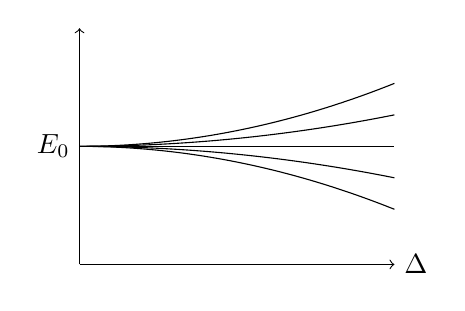
\begin{tikzpicture}
	\draw[->] (0,0) -- (4,0) node[right]{$\Delta$};
	\draw[->] (0,0) -- (0,3);
	\node[left] at (0,1.5) {$E_{0}$};
	\draw[domain=0:4,samples=200] plot (\x, {1.5+0.05*(\x)^2});
	\draw[domain=0:4,samples=200] plot (\x, {1.5+0.025*(\x)^2});
	\draw[domain=0:4,samples=200] plot (\x, {1.5});
	\draw[domain=0:4,samples=200] plot (\x, {1.5-0.025*(\x)^2});
	\draw[domain=0:4,samples=200] plot (\x, {1.5-0.05*(\x)^2});
\end{tikzpicture}
\end{center}
Energy levels now form a continuous band of values from $E_{0}-2\Delta$ to $E_{0}+2\Delta$. When $\Delta=0$, the single eigenvalue $E_{0}$ is recovered.\\

To understand the physical meaning of $\ket{\theta}$, consider wavefunction $\ip{x'}{\theta}$
\begin{equation}
\begin{aligned}
\mel{x'}{\vb{T}(a)}{\theta}&=\mel{\theta}{\vb{T}^{\dagger}(a)}{x'}^{*}\\
&=\ip{\theta}{x'-a}^{*}\\
&=\ip{x'-a}{\theta}\\
\mel{x'}{\vb{T}(a)}{\theta}&=e^{-i\theta}\ip{x'}{\theta}\\
\therefore \ip{x'-a}{\theta}&=e^{-i\theta}\ip{x'}{\theta}
\end{aligned}
\end{equation}
The most general solution of this equation is
\begin{equation}
\ip{x'}{\theta}=e^{ikx'}U_{k}(x')
\end{equation}
with $\theta=ka$ and $U_{k}(x'+a)=U_{k}(x')$. Thus
\begin{equation}
\begin{aligned}
\ip{x'-a}{\theta}&=e^{ik(x'-a)}U_{k}(x'-a)\\
&=e^{-ika}e^{ikx'}U_{k}(x')\\
&=e^{-i\theta}\ip{x'}{\theta}\qq{as required}
\end{aligned}
\end{equation}
Note that $U_{k}(x')$ is a Bloch wavefunction.
\begin{equation}
e^{ik(x'-a)}U_{k}(x'-a)=e^{ikx'}U_{k}(x')e^{-ika}
\end{equation}
This is an important condition called \ul{Bloch's theorem}. The wavefunction of $\ket{\theta}$, which is an eigenket of $\vb{T}(a)$ can be written as a plane wave $e^{ikx'}$ times a periodic function with periodicity of $a$. Note we only used the fact that $\vb{T}(a)\ket{\theta}=e^{-i\theta}\ket{\theta}$. This theorem still holds even if the tight-binding approximation breaks down.\\

Thus, physically, the wavefunction is a plane wave with propagation wave vector $k$ modulated by periodic function $U_{k}(x')$. Since $\theta$ varies from $-\pi$ to $\pi$, the wave vector varies from $-\frac{\pi}{a}$ to $\frac{\pi}{a}$. The energy eigenvalue $E(k)$ is now
\begin{equation}
E(k)=E_{0}-2\Delta\cos(ka)
\end{equation}
The energy eigenvalue equation is independent of the detailed shape of the potential as long as the tight-binding approximation is valid. ote there is also a cutoff in wave vector $k$ of the Bloch wavefunction given by $\abs{k}=\frac{\pi}{a}$. The energy eigenvalue equation defines a band dispersion of the tight-binding approximation. These allowed energies form a continuous band called the \ul{Brillouin zone}. $-\frac{\pi}{a}\leq k\leq \frac{\pi}{a}$ corresponds with the first Brillouin zone.\\

One calls $\hbar k$ the crystal momentum and its conservation is a consequence of discrete lattice translation symmetry.

\subsection{Symmetries of Time-Reversal}
Due to the subtlety and novelty of this symmetry, we shall start with considering a case from classical mechanics. Suppose a particle is moving along a trajectory in the presence of an external force.
\begin{center}
\begin{tikzpicture}
	\draw[domain=0:3,samples=200] plot (\x, {-0.25*(\x)^2});
	\draw[domain=7:10,samples=200] plot (\x, {-0.25*(\x-7)^2});
	\draw[->,red,thick,text=black] (1,-0.25) node[above right,xshift=0.3cm] {$\vec{p}$, $t=0$} -- (1.5,-0.5);
	\draw[->,red,thick,text=black] (8,-0.25) node[above right,xshift=0.3cm] {$-\vec{p}$, $t=0$} -- (7.5,0);
\end{tikzpicture}
\end{center}
Suppose at time $t=0$ we stop the particle and reverse its momentum ($\vec{p}\eval_{t=0}\rightarrow-\vec{p}\eval_{t=0}$). In the absence of friction, the particle simply retraces its trajectory in the opposite direction. In other words, for the equation
\begin{equation}
m\dv[2]{\vec{x}}{t}=-\vec{\nabla}V(\vec{x})
\end{equation}
Under the time-reversal map $t\rightarrow-t$, the equations of motion do not change. Thus, both $\vec{x}(t)$ and $\vec{x}(-t)$ are solutions to the equations of motion. The laws of motion for a particle in a potential $V(\vec{x})$ are invariant with respect to time-reversal.\\

Consider now a charged particle moving in an external magnetic field. This generates the Lorentz force
\begin{equation}
\vec{F}=\frac{e}{c}\vec{v}\times\vec{B}\qq{in CGS units}
\end{equation}
\begin{center}
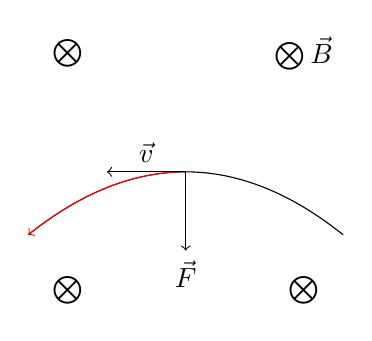
\begin{tikzpicture}
	\node at (-1.5,2) {$\bigotimes$};
	\node at (1.5,2) {$\bigotimes \vec{B}$};
	\node at (-1.5,-1) {$\bigotimes$};
	\node at (1.5,-1) {$\bigotimes$};
	\draw[domain=-2:2,samples=200] plot (\x, {0.5-0.2*(\x)^2});
	\draw[domain=-2:0,samples=200,<-,red] plot (\x, {0.5-0.2*(\x)^2});
	\draw[->] (0,0.5) -- (0,-0.5) node[below] {$\vec{F}$};
	\draw[->] (0,0.5) -- node[above] {$\vec{v}$} (-1,0.5);
\end{tikzpicture}
\end{center}
Note $\vec{B}$ points into the page. Suppose the particle is stopped and the direction of velocity is reversed. Taking $\vec{B}$ to be the same sign, $\vec{F}$ changes sign.

\begin{center}
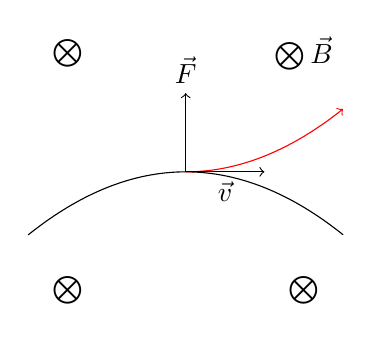
\begin{tikzpicture}
	\node at (-1.5,2) {$\bigotimes$};
	\node at (1.5,2) {$\bigotimes \vec{B}$};
	\node at (-1.5,-1) {$\bigotimes$};
	\node at (1.5,-1) {$\bigotimes$};
	\draw[domain=-2:2,samples=200] plot (\x, {0.5-0.2*(\x)^2});
	\draw[domain=0:2,samples=200,->,red] plot (\x, {0.5+0.2*(\x)^2});
	\draw[->] (0,0.5) -- (0,1.5) node[above] {$\vec{F}$};
	\draw[->] (0,0.5) -- node[below] {$\vec{v}$} (1,0.5);
\end{tikzpicture}
\end{center}
The time-reversal trajectory won't be the same. The motion of a charge particle in an external magnetic field violates time-reversal invariance, assuming the field itself is fixed.\\

Consider now a quantum mechanical particle moving in potential $V(\vec{x})$. The equations of motion are determined by the Schr\"{o}dinger equation.
\begin{equation}
i\hbar\pdv{\psi}{t}=\qty(-\frac{\hbar^{2}\nabla^{2}}{2m}+V(\vec{x}))\psi
\end{equation}
If $\psi(\vec{x},t)$ is a solution, simply taking $\psi(\vec{x},-t)$ will not be a solution to the equation, as the left-side picks up an extra negative sign, while the right-hand side doesn't. However, $\psi^{*}(\vec{x},-t)$ is a solution, which can be verified by taking the complex conjugate of the Schr\"{o}dinger equation.
\begin{equation}
i\hbar\pdv{\psi^{*}(\vec{x},-t)}{(-t)}=\qty(-\frac{\hbar^{2}\nabla^{2}}{2m}+V(\vec{x}))\psi^{*}(\vec{x},-t)
\end{equation}
Thus, time-reversal in quantum mechanics is tied to complex conjugation. Let us introduce the time-reversal operator $\Theta$. If $\ket{\psi}$ is an arbitrary state, then $\Theta\ket{\psi}$ corresponds to the time-reversal state.\\

Suppose at time $t=0$, the system is in state $\ket{\psi}$. Applying the infinitesimal time translation operator
\begin{equation}
\ket{\psi,t=\delta t}=\qty(\mathbb{I}-\frac{i}{\hbar}\vb{H}\delta t)\ket{\psi}
\end{equation}
Suppose at time $t=0$, one applies the time-reversal operator and then lets the system to evolve under $\vb{H}$. Thus, the state is
\[
\qty(\mathbb{I}-\frac{i}{\hbar}\vb{H}\delta t)\Theta\ket{\psi}
\]
If motion obeys time-reversal, then the state must be of the form
\[
\Theta\ket{\psi,t=-\delta t}
\]
Thus
\begin{equation}
\begin{aligned}
\qty(\mathbb{I}-\frac{i}{\hbar}\vb{H}\delta t)\Theta\ket{\psi}&=\Theta\ket{\psi,t=-\delta t}\\
&=\Theta\qty(\mathbb{I}-\frac{i}{\hbar}\vb{H}(-\delta t))\ket{\psi}\\
&=\Theta\qty(\mathbb{I}+\frac{i}{\hbar}\vb{H}\delta t)\ket{\psi}
\end{aligned}
\end{equation}
This must be true for an arbitrary ket $\ket{\psi}$. Simplifying
\begin{equation}
\begin{aligned}
\qty(\mathbb{I}-\frac{i}{\hbar}\vb{H}\delta t)\Theta&=\Theta\qty(\mathbb{I}+\frac{i}{\hbar}\vb{H}\delta t)\\
-i\vb{H}\Theta&=\Theta i\vb{H}
\end{aligned}
\end{equation}
Let us argue that $\Theta$ is not unitary. If $\Theta$ is unitary, $i$ can be canceled and we obtain
\begin{equation}
-\vb{H}\Theta=\Theta\vb{H}
\end{equation}
Consider an energy eigenket $\ket{n}$ with energy eigenvalue $E_{n}$. The time-reversed state would be $\Theta\ket{n}$.
\begin{equation}
\vb{H}\Theta\ket{n}=-\Theta\vb{H}\ket{n}=(-E_{n})\Theta\ket{n}
\end{equation}
This mean $\Theta\ket{n}$ is an eigenket with energy $-E_{n}$. Thus, time-reversal would change the sign of the energy This is nonsensical. For example, for a free particle, the time-reversal would simply the reverse the direction of motion. However, its energy should still remain the same. Moreover
\begin{equation}
\vb{H}=\frac{\vec{\vb{p}}^{2}}{2m}
\end{equation}
Under time-reversal, $\vb{H}$ should remain the same ($\vec{\vb{p}}^{2}$ doesn't change sign under time-reversal). Thus, $\Theta$ must act on $i$ as well. It is not a unitary operator, but rather an anti-unitary operator.\\

For a unitary operator $U$
\begin{equation}
\begin{aligned}
\ket*{\widetilde{\psi}}&=U\ket{\psi},\quad\ket*{\widetilde{\phi}}=U\ket{\phi}\\
\ip*{\widetilde{\phi}}{\widetilde{\psi}}&=\mel{\phi}{U^{\dagger}U}{\psi}=\ip{\phi}{\psi}
\end{aligned}
\end{equation}
In the case of time-reversal, since $\Theta$ is not unitary, this cannot be the case. Instead, we have
\begin{equation}
\abs{\ip*{\widetilde{\phi}}{\widetilde{\psi}}}^{2}=\abs{\ip{\phi}{\psi}}^{2}
\end{equation}
Thus, one can have now
\begin{equation}
\ip*{\widetilde{\phi}}{\widetilde{\psi}}=\ip{\phi}{\psi}^{*}\qq{instead of}\ip*{\widetilde{\phi}}{\widetilde{\psi}}=\ip{\phi}{\psi}
\end{equation}

\definition{Suppose $\ket*{\widetilde{\phi}}=\theta\ket{\phi}$ and $\ket*{\widetilde{\psi}}=\theta\ket{\psi}$. $\theta$ is \ul{anti-unitary} if $\ip*{\widetilde{\phi}}{\widetilde{\psi}}=\ip{\phi}{\psi}^{*}$ and $\theta\qty(c_{1}\ket{\psi}+c_{2}\ket{\phi})=c_{1}^{*}\theta\ket{\psi}+c_{2}^{*}\theta\ket{\phi}$.}

One can show that an anti-unitary operator may be written as $\theta=UK$, where $U$ is a unitary operator and $K$ is a \ul{complex conjugation operator} that complex conjugates all complex numbers to its right.
\begin{equation}
\therefore Kc\ket{\alpha}=c^{*}K\ket{\alpha},\quad c\in\mathbb{C}
\end{equation}
If $\ket{\psi}=\sum_{a'}\ket{a'}\ip{a'}{\psi}$ then
\begin{equation}
K\ket{\psi}=\sum_{a'}\ket{a'}\ip{a'}{\psi}^{*}
\end{equation}
Therefore
\begin{equation}
\begin{aligned}
\theta(c_{1}\ket{\psi}+c_{2}\ket{\phi})&=UK(c_{1}\ket{\psi}+c_{2}\ket{\phi})\\
&=c_{1}^{*}UK\ket{\psi}+c_{2}^{*}UK\ket{\phi}\\
&=c_{1}^{*}\theta\ket{\psi}+c_{2}^{*}\theta\ket{\phi}\qq{as before}
\end{aligned}
\end{equation}
Thus, $\theta=UK$ is valid.\\

One can now write $\ket*{\widetilde{\psi}}$ as
\begin{equation}
\begin{aligned}
\ket*{\widetilde{\psi}}&=\theta\ket{\psi}\\
&=UK\ket{\psi}\\
&=UK\sum_{a'}\ket{a'}\ip{a'}{\psi}\\
&=\sum_{a'}\ip{a'}{\psi}^{*}U\ket{a'}\\
&=\sum_{a'}\ip{\psi}{a'}U\ket{a'}
\end{aligned}
\end{equation}
Similarly
\begin{equation}
\ket*{\widetilde{\phi}}=\theta\ket{\phi}=\sum_{a'}\ip{\phi}{a'}U\ket{a'}
\end{equation}
Taking the Hermitian conjugate
\begin{equation}
\bra*{\widetilde{\phi}}=\sum_{a'}\ip{\phi}{a'}^{*}\bra{a'}U^{\dagger}=\sum_{a'}\ip{a'}{\phi}\bra{a'}U^{\dagger}
\end{equation}
Therefore
\begin{equation}
\begin{aligned}
\ip*{\widetilde{\phi}}{\widetilde{\psi}}&=\sum_{a'a''}\ip{a'}{\phi}\ip{\psi}{a''}\mel{a'}{U^{\dagger}U}{a''}\\
&=\sum_{a'a''}\ip{a'}{\phi}\ip{\psi}{a''}\ip{a'}{a''}\\
&=\sum_{a'a''}\ip{a'}{\phi}\ip{\psi}{a''}\delta_{a'a''}\\
&=\sum_{a'}\ip{a'}{\phi}\ip{\psi}{a'}\\
&=\ip{\psi}{\phi}\\
&=\ip{\phi}{\psi}^{*}
\end{aligned}
\end{equation}
Since $\Theta$ is anti-unitary, $\Theta i=-i\Theta$. Thus, from before
\begin{equation}
\begin{aligned}
-i\vb{H}\Theta&=\Theta i\vb{H}\\
\vb{H}\Theta&=\Theta\vb{H}
\end{aligned}
\end{equation}
Thus, $\vb{H}$ commutes with $\Theta$ and $\comm{\vb{H}}{\Theta}=0$.\\

Let $\ket*{\widetilde{\psi}}=\Theta\ket{\psi}$ and $\ket*{\widetilde{\phi}}=\Theta\ket{\phi}$. Let $\vb{A}$ be some operator that is not necessarily Hermitian. Let $\ket{\xi}=\vb{A}^{\dagger}\ket{\phi}$. Thus, $\bra{\xi}=\bra{\phi}\vb{A}$.\\

Therefore
\begin{equation}
\begin{aligned}
\mel{\phi}{\vb{A}}{\psi}&=\ip{\xi}{\psi}\\
&=\ip*{\widetilde{\xi}}{\widetilde{\psi}}^{*}\\
&=\ip*{\widetilde{\psi}}{\widetilde{\xi}}\\
&=\mel*{\widetilde{\psi}}{\Theta}{\xi}\\
&=\mel*{\widetilde{\psi}}{\Theta \vb{A}^{\dagger}}{\phi}\\
&=\mel*{\widetilde{\psi}}{\Theta \vb{A}^{\dagger}\Theta^{-1}\Theta}{\phi}\\
&=\mel*{\widetilde{\psi}}{\Theta\vb{A}^{\dagger}\Theta^{-1}}{\widetilde{\phi}}
\end{aligned}
\end{equation}
If $\vb{A}$ is Hermitian
\begin{equation}
\begin{aligned}
\mel{\phi}{\vb{A}}{\psi}=\mel*{\widetilde{\psi}}{\Theta\vb{A}\Theta^{-1}}{\widetilde{\phi}}
\end{aligned}
\end{equation}
The time-reversal operator of $\vb{A}$ is $\Theta\vb{A}\Theta^{-1}$. If $\Theta\vb{A}\Theta^{-1}=\vb{A}$, $\vb{A}$ is even under time-reversal. If $\Theta\vb{A}\Theta^{-1}=-\vb{A}$, $\vb{A}$ is odd under time-reversal. Therefore
\begin{equation}
\begin{aligned}
\mel{\phi}{\vb{A}}{\psi}&=\pm\mel*{\widetilde{\psi}}{\vb{A}}{\widetilde{\phi}}\\
&=\pm\mel*{\widetilde{\phi}}{\vb{A}}{\widetilde{\psi}}^{*}
\end{aligned}
\end{equation}
If $\ket{\phi}=\ket{\psi}$
\begin{equation}
\mel{\psi}{\vb{A}}{\psi}=\pm\mel*{\widetilde{\psi}}{\vb{A}}{\widetilde{\psi}}\qq{(expectation value)}
\end{equation}
Consider linear momentum operator $\vec{\vb{p}}$. By physical arguments, under time-reversal, the expectation value of $\vec{\vb{p}}$ changes sign
\begin{equation}
\mel{\psi}{\vec{\vb{p}}}{\psi}=-\mel*{\widetilde{\psi}}{\vec{\vb{p}}}{\widetilde{\psi}}
\end{equation}
Thus, $\vec{\vb{p}}$ is odd under time-reversal, $\Theta\vec{\vb{P}}\Theta^{-1}=-\vec{\vb{p}}$.
\begin{equation}
\begin{aligned}
\vec{\vb{p}}\Theta\ket{\vec{p}\,'}&=-\Theta\vec{\vb{p}}\Theta^{-1}\Theta\ket{\vec{p}\,'}\\
&=-\Theta\vec{\vb{p}}\ket{\vec{p}\,'}\\
&=-\vec{p}\,'\Theta\ket{\vec{p},'}
\end{aligned}
\end{equation}
Thus, $\Theta\ket{\vec{p}\,'}=\ket{-\vec{p}\,'}$.\\

Similarly, by physical arguments, under time-reversal, the expectation value of the position operator $\vec{\vb{x}}$ does not change sign under time-reversal.
\begin{equation}
\mel{\psi}{\vec{\vb{x}}}{\psi}=\mel*{\widetilde{\psi}}{\vec{\vb{x}}}{\widetilde{\psi}}
\end{equation}
Thus, $\vec{\vb{x}}$ is even under time-reversal, $\Theta\vec{\vb{x}}\Theta^{-1}=\vec{\vb{x}}$.
\begin{equation}
\begin{aligned}
\vec{\vb{x}}\Theta\ket{\vec{x}\,'}&=\Theta\vec{\vb{x}}\Theta^{-1}\Theta\ket{\vec{x}\,'}\\
&=\Theta\vec{\vb{x}}\ket{\vec{x}\,'}\\
&=\vec{x}\,'\Theta\ket{\vec{x}\,'}
\end{aligned}
\end{equation}
Thus, $\Theta\ket{\vec{x}\,'}=\ket{\vec{x}\,'}$.\\

Checking the invariance of the commutation relation under time-reversal
\begin{equation}
\begin{aligned}
\comm{\vb{x}_{i}}{\vb{p}_{j}}&=i\hbar\delta_{ij}\\
\comm{\vb{x}_{i}}{\vb{p}_{j}}\ket{\psi}&=i\hbar\delta_{ij}\ket{\psi}\\
\Theta\comm{\vb{x}_{i}}{\vb{p}_{j}}\ket{\psi}&=\Theta i\hbar\delta_{ij}\ket{\psi}\\
\Theta\comm{\vb{x}_{i}}{\vb{p}_{j}}\ket{\psi}&=-i\hbar\delta_{ij}\Theta\ket{\psi}
\end{aligned}
\end{equation}
Since this is true for arbitrary state $\ket{\psi}$
\begin{equation}
\begin{aligned}
\Theta\comm{\vb{x}_{i}}{\vb{p}_{j}}\Theta^{-1}&=-i\hbar\delta_{ij}\\
\Theta\comm{\vb{x}_{i}}{\vb{p}_{j}}\Theta^{-1}&=-\comm{\vb{x}_{i}}{\vb{p}_{j}}
\end{aligned}
\end{equation}
This is expected, as $\Theta\comm{\vb{x}_{i}}{\vb{p}_{j}}\Theta^{-1}=\comm{\vb{x}_{i}}{-\vb{p}_{j}}$. Thus, $\Theta$ preserves the $\vec{\vb{x}}$ and $\vec{\vb{p}}$ commutation relation. Similarly, the preserve $\comm{\vb{J}_{i}}{\vb{J}_{j}}=i\hbar\varepsilon_{ijk}\vb{J}_{k}$, $\vec{\vb{J}}$ must be odd under time-reversal
\begin{equation}
\Theta\vec{\vb{J}}\Theta^{-1}=-\vec{\vb{J}}
\end{equation}
This is consistent with $\vec{\vb{J}}=\vec{\vb{x}}\times\vec{\vb{p}}$ for spinless systems.\\

Let us see that this gives the same transformation rules for wavefunctions as found earlier
\begin{equation}
\begin{aligned}
\ket{\psi}&=\int\dd{\vec{x}\,'}\ket{\vec{x}\,'}\ip{\vec{x}\,'}{\psi}\\
\Theta\ket{\psi}&=\int\dd{\vec{x}\,'}\Theta\ket{\vec{x}\,'}\ip{\vec{x}\,'}{\psi}\\
&=\int\dd{\vec{x}\,'}\ip{\vec{x}\,'}{\psi}^{*}\Theta\ket{\vec{x}\,'}\\
&=\int\dd{\vec{x}\,'}\ip{\vec{x}\,'}{\psi}^{*}\ket{\vec{x}\,'}\\
&=\int\dd{\vec{x}\,'}\ket{\vec{x}\,'}\ip{\vec{x}\,'}{\psi}^{*}
\end{aligned}
\end{equation}
Thus, $\psi(\vec{x}\,')\rightarrow\psi^{*}(\vec{x}\,')$ as before. Moreover
\begin{equation}
\begin{aligned}
\mel{\vec{x}\,''}{\Theta}{\psi}&=\int\dd{\vec{x}\,'}\ip{\vec{x}\,''}{\vec{x}\,'}\ip{\vec{x}\,'}{\psi}^{*}\\
&=\int\dd{\vec{x}\,'}\delta(\vec{x}\,''-\vec{x}\,')\ip{\vec{x}\,'}{\psi}^{*}\\
&=\ip{\vec{x}\,''}{\psi}^{*}
\end{aligned}
\end{equation}
Similarly, one can find through the same process
\begin{equation}
\mel{\vec{p}\,''}{\Theta}{\psi}=\ip{-\vec{p}\,''}{\psi}^{*}
\end{equation}

\theorem{Suppose the Hamiltonian is invariant under time-reversal and its energy eigenket is non-degenerate, then the corresponding wavefunction may be chosen to be real.}

\proof{\begin{equation}
\vb{H}\Theta\ket{n}=\Theta\vb{H}\ket{n}=E_{n}\Theta\ket{n}
\end{equation}
Thus, $\ket{n}$ and $\Theta\ket{n}$ have the same energy. Since $\ket{n}$ is non-degenerate, $\ket{n}=\Theta\ket{n}$. However
\begin{equation}
\ip{\vec{x}\,'}{n}=\mel{\vec{x}\,'}{\Theta}{n}=\ip{\vec{x}\,'}{n}
\end{equation}
Thus, $\ip{\vec{x}\,'}{n}$ is real.
}

\subsection{Time-Reversal of Spin-$\frac{1}{2}$ Systems}
Consider a particle with spin-$\frac{1}{2}$. Consider an arbitrary spinor, which can be thought of as an eigenket of $\vec{\vb{S}}\cdot\hat{n}$, where
\begin{equation}
\hat{n}=(\sin\theta\cos\varphi,\sin\theta\sin\varphi,\cos\theta)
\end{equation}
This can be found by finding eigenket $\ket{\up}$ of $\vb{S}_{z}$ and rotating it to direction $\hat{n}$. Thus, the eigenket is
\begin{equation}
\ket{\hat{n},\up}=e^{-\frac{i}{\hbar}\vb{S}_{z}\varphi}e^{-\frac{i}{\hbar}\vb{S}_{y}\theta}\ket{\up}
\end{equation}
From before
\begin{equation}
\Theta\vb{S}\Theta^{-1}=-\vec{\vb{S}}\implies \Theta\vec{\vb{S}}=-\vec{\vb{S}}\Theta
\end{equation}
Thus
\begin{equation}
\begin{aligned}
\Theta\ket{\hat{n},\up}&=\Theta e^{-\frac{i}{\hbar}\vb{S}_{z}\varphi}e^{-\frac{i}{\hbar}\vb{S}_{y}\theta}\ket{\up}\\
&=e^{-\frac{i}{\hbar}\vb{S}_{z}\varphi}e^{-\frac{i}{\hbar}\vb{S}_{y}\theta}\ket{\up}\\
&\quad\explain{Note that $\Theta\vec{\vb{S}}=-\vec{\vb{S}}\Theta$, but $\Theta i=-i\Theta$, so the negative signs cancel.}
\end{aligned}
\end{equation}
What is $\Theta\ket{\up}$?
\begin{equation}
\vb{S}_{z}\Theta\ket{\up}=-\Theta\vb{S}_{z}\ket{\up}=-\frac{\hbar}{2}\Theta\ket{\up}
\end{equation}
Thus, $\Theta\ket{\up}$ is an eigenket of $\vb{S}_{z}$ with eigenvalues $-\frac{\hbar}{2}$. Thus
\begin{equation}
\Theta\ket{\up}=e^{i\eta}\ket{\dn}\qq{where $e^{i\eta}$ is an arbitrary phase factor}
\end{equation}
Therefore
\begin{equation}
\begin{aligned}
\Theta\ket{\hat{n},\up}&=e^{-\frac{i}{\hbar}\vb{S}_{z}\varphi}e^{-\frac{i}{\hbar}\vb{S}_{y}\theta}e^{i\eta}\ket{\dn}\\
&=e^{i\eta}\ket{\hat{n},\dn}
\end{aligned}
\end{equation}
where
\begin{equation}
\begin{aligned}
\ket{\hat{n},\dn}&=e^{-\frac{i}{\hbar}\vb{S}_{z}\varphi}e^{-\frac{i}{\hbar}\vb{S}_{y}\theta}\ket{\dn}\\
&=\qty(\cos\frac{\varphi}{2}-i\sigma_{z}\sin\frac{\varphi}{2})\qty(\cos\frac{\theta}{2}-i\sigma_{y}\sin\frac{\theta}{2})\ket{\dn}\\
&=\mqty[e^{-\frac{i\varphi}{2}} & 0 \\ 0 & e^{\frac{i\varphi}{2}}]\mqty[\cos\frac{\theta}{2} & -\sin\frac{\theta}{2} \\ \sin\frac{\theta}{2} & \cos\frac{\theta}{2}]\mqty[0 \\ 1]\\
&=\mqty[-e^{-\frac{i\varphi}{2}}\sin\frac{\theta}{2} \\ e^{\frac{i\varphi}{2}}\cos\frac{\theta}{2}]
\end{aligned}
\end{equation}
Note that similarly
\begin{equation}
\ket{\hat{n},\up}=\mqty[-e^{-\frac{i\varphi}{2}}\cos\frac{\theta}{2} \\ e^{\frac{i\varphi}{2}}\sin\frac{\theta}{2}]
\end{equation}
Therefore
\begin{equation}
\begin{aligned}
\ket{\hat{n}(\theta,\varphi),\dn}&=\ket{\hat{n}(\theta+\pi,\varphi),\up}\\
&=e^{-\frac{i}{\hbar}\vb{S}_{z}\varphi}e^{-\frac{i}{\hbar}\vb{S}_{y}(\theta+\pi)}\ket{\up}
\end{aligned}
\end{equation}
Thus
\begin{equation}
\begin{aligned}
\Theta\ket{\hat{n},\up}&=r^{-\frac{i}{\hbar}\vb{S}_{z}\varphi}e^{-\frac{i}{\hbar}\vb{S}_{y}\theta}e^{i\eta}\ket{\dn}\\
&=e^{i\eta}\ket{\hat{n},\dn}\\
&=e^{i\eta}e^{-\frac{i}{\hbar}\vb{S}_{z}\varphi}e^{-\frac{i}{\hbar}\vb{S}_{y}(\theta+\pi)}\ket{\up}
\end{aligned}
\end{equation}
Since $\Theta\ket{\hat{n},\up}=\Theta e^{-\frac{i}{\hbar}\vb{S}_{z}\varphi}e^{-\frac{i}{\hbar}\vb{S}_{y}\theta}\ket{\up}$
\begin{equation}
\Theta e^{-\frac{i}{\hbar}\vb{S}_{z}\varphi}e^{-\frac{i}{\hbar}\vb{S}_{y}\theta}\ket{\up}=e^{i\eta}e^{-\frac{i}{\hbar}\vb{S}_{z}\varphi}e^{-\frac{i}{\hbar}\vb{S}_{y}(\theta+\pi)}\ket{\up}
\end{equation}
Additionally
\begin{equation}
\begin{aligned}
\Theta&=UK\\
&=e^{i\eta}e^{-\frac{i}{\hbar}\vb{S}_{y}\pi}K\\
&=e^{i\eta}e^{-\frac{i}{2}\sigma_{y}\pi}K\\
&=e^{i\eta}\qty(\cos\frac{\pi}{2}-i\sigma_{y}\sin\frac{\pi}{2})K\\
&=-ie^{i\eta}\sigma_{y}K
\end{aligned}
\end{equation}
\begin{equation}
\begin{aligned}
\Theta\ket{\up}&=-ie^{i\eta}\sigma_{y}\ket{\up}\\
&=-i\mqty[0 & -i \\ i & 0]\mqty[1\\0]e^{i\eta}\\
&=e^{i\eta}\ket{\dn}\\
\Theta\ket{\dn}&=-ie^{i\eta}\sigma_{y}\ket{\dn}\\
&=-i\mqty[0 & -i\\ i & 0]\mqty[0\\1]e^{i\eta}\\
&=-e^{i\eta}\ket{\up}
\end{aligned}
\end{equation}
For $\ket{z}=z_{\up}\ket{\up}+z_{\dn}\ket{\dn}$
\begin{equation}
\Theta\ket{z}=z_{\up}^{*}e^{i\eta}\ket{\dn}-z_{\dn}^{*}e^{i\eta}\ket{\up}
\end{equation}
Applying $\Theta$ again
\begin{equation}
\begin{aligned}
\Theta^{2}\ket{z}&=\Theta\qty(z_{\up}^{*}e^{i\eta}\ket{\dn}-z_{\dn}^{*}e^{i\eta}\ket{\up})\\
&=z_{\up}e^{-i\eta}\Theta\ket{\dn}-z_{\dn}e^{-i\eta}\Theta\ket{\up}\\
&=-z_{\up}\ket{\up}-z_{\dn}\ket{\dn}\\
&=-\ket{z}
\end{aligned}
\end{equation}
Thus, for spin-$\frac{1}{2}$ particles
\begin{equation}
\Theta^{2}=-\mathbb{I}
\end{equation}
In general, for a spin-$j$ particle
\begin{equation}
\Theta^{2}=(-\mathbb{I})^{2j}
\end{equation}

\subsection{Time-Reversal Invariance and Kramer's Theorem}
Consider a time-reversal invariant system where $\comm{\Theta}{\vb{H}}=0$. Thus, $\vb{H}$ is even under time-reversal and
\begin{equation}
\Theta\vb{H}\Theta^{-1}=\vb{H}
\end{equation}
Consider the eigensystem $\vb{H}\ket{n}=E_{n}\ket{n}$. Thus
\begin{equation}
\begin{aligned}
\vb{H}\Theta\ket{n}&=\Theta\vb{H}\ket{n}\\
&=E_{n}\vb{H}\ket{n}
\end{aligned}
\end{equation}
Assuming $\ket{n}$ is non-degenerate
\begin{equation}
\begin{aligned}
\Theta\ket{n}&=e^{i\delta}\ket{n}\\
\Theta^{2}\ket{n}&=\Theta e^{i\delta}\ket{n}=e^{-i\delta}\Theta\ket{n}=e^{-i\delta}e^{i\delta}\ket{n}=\ket{n}\\
\therefore\Theta^{2}&=\mathbb{I}
\end{aligned}
\end{equation}
However, for a spin-$j$ particle, we found $\Theta^{2}=(-\mathbb{I})^{2j}$. For half-integer $j$, $\Theta^{2}=-\mathbb{I}$, leading to a contradiction. Thus, the assumption that $\ket{n}$ is non-degenerate is wrong for half-integers $j$. This leads to \ul{Kramer's theorem}, which states that in a time-reversal invariant system with half-integer spin-$j$, all eigenstates of $\vb{H}$ are degenerate.

\newpage
\section{Time-Dependent Hamiltonian}
Thus far, Hamiltonians have been taken to be time-independent. However, many important problems in quantum mechanics involve such time-dependence, in particular problems involving response of the system to an externally applied probe.\\

Take the time-dependent Hamiltonian to be
\begin{equation}
\vb{H}=\vb{H}_{0}+V(t)\qq{where $\vb{H}_{0}$ is time-independent}
\end{equation}
Contrast this with the time-independent Hamiltonian
\begin{equation}
\vb{H}=\frac{(\vec{\vb{p}})^{2}}{2m}+V(\vec{\vb{x}})
\end{equation}
Typically, we take the $V(t)=0$ case to be solved in the sense that the energy eigenkets and eigenvalues are known and defined by
\begin{equation}
\vb{H}_{0}\ket{n}=E_{n}\ket{n}
\end{equation}
Recall for the time-evolution of a state for a time-independent Hamiltonian is
\begin{equation}
\ket{\psi,t}_{\trm{S}}=e^{-\frac{i}{\hbar}\vb{H}t}\ket{\psi}
\end{equation}
for a state in the Schr\"{o}dinger picture. In the Heisenberg picture, the states are
\begin{equation}
\ket{\psi}_{\trm{H}}=\ket{\psi}=e^{\frac{i}{\hbar}\vb{H}t}\ket{\psi,t}_{\trm{S}}
\end{equation}
with the operators being time-dependent
\begin{equation}
\vb{A}^{(\trm{H})}(t)=e^{\frac{i}{\hbar}\vb{H}t}\vb{A}^{(\trm{S})}e^{-\frac{i}{\hbar}\vb{H}t}
\end{equation}
The time-evolution of the operator is given by
\begin{equation}
\dv{\vb{A}^{(\trm{H})}}{t}=\frac{i}{\hbar}\comm{\vb{H}}{\vb{A}^{(\trm{H})}}
\end{equation}

In problems with explicit time-dependence of the Hamiltonian, it becomes convenient to use the \ul{interaction picture}, where
\begin{equation}
\ket{\psi,t}_{\trm{I}}=e^{\frac{i}{\hbar}\vb{H}_{0}t}\ket{\psi,t}_{\trm{S}}
\end{equation}
is modified by the time-independent component of the Hamiltonian. Likewise, the operators are given by
\begin{equation}
\begin{aligned}
\tensor[_{\trm{S}}]{\mel{\psi,t}{\vb{A}^{(\trm{S})}}{\psi,t}}{_{\trm{S}}}&=\tensor[_{\trm{I}}]{\mel{\psi,t}{e^{\frac{i}{\hbar}\vb{H}_{0}t}\vb{A}^{(S)}e^{-\frac{i}{\hbar}\vb{H}_{0}t}}{\psi,t}}{_{\trm{I}}}\\
\therefore\vb{A}^{(\trm{I})}(t)&=e^{\frac{i}{\hbar}\vb{H}_{0}t}\vb{A}^{(\trm{S})}e^{-\frac{i}{\hbar}\vb{H}_{0}t}
\end{aligned}
\end{equation}
This picture can be thought of as being an intermediate between the two pictures before. Note that the states and operators in the interaction picture coincide with those of the Heisenberg picture when $\vb{H}=\vb{H}_{0}$ (i.e. $V(t)=0$).\\

Modifying the Schr\"{o}dinger equation
\begin{equation}
\begin{aligned}
i\hbar\pdv{t}\ket{\psi,t}_{\trm{I}}&=i\hbar\pdv{t}\qty(e^{\frac{i}{\hbar}\vb{H}_{0}t}\ket{\psi,t}_{\trm{S}})\\
&=-\vb{H}_{0}e^{\frac{i}{\hbar}\vb{H}_{0}t}\ket{\psi,t}_{\trm{S}}+e^{\frac{i}{\hbar}\vb{H}_{0}t}i\hbar\pdv{t}\ket{\psi,t}_{\trm{S}}\\
&=-\vb{H}_{0}e^{\frac{i}{\hbar}\vb{H}_{0}t}\ket{\psi,t}_{\trm{S}}+e^{\frac{i}{\hbar}\vb{H}_{0}t}\vb{H}\ket{\psi,t}_{\trm{S}}\\
&\quad\explain{By the Schr\"{o}dinger equation for $\ket{\psi,t}_{\trm{S}}$}\\
&=-\vb{H}_{0}e^{\frac{i}{\hbar}\vb{H}_{0}t}\ket{\psi,t}_{\trm{S}}+e^{\frac{i}{\hbar}\vb{H}_{0}t}\qty(\vb{H}_{0}+V(t))\ket{\psi,t}_{\trm{S}}\\
&=e^{\frac{i}{\hbar}\vb{H}_{0}t}V(t)\ket{\psi,t}_{\trm{S}}\\
&\quad\explain{Since $\vb{H}_{0}$ commutes with $e^{\frac{i}{\hbar}\vb{H}_{0}t}$}\\
&=e^{\frac{i}{\hbar}\vb{H}_{0}t}V(t)e^{-\frac{i}{\hbar}\vb{H}_{0}t}\ket{\psi,t}_{\trm{I}}\\
\therefore i\hbar\pdv{t}\ket{\psi,t}_{\trm{I}}&=V^{\trm{(I)}}(t)\ket{\psi,t}_{\trm{I}}
\end{aligned}
\end{equation}
where
\begin{equation}
V^{(I)}(t)=e^{\frac{i}{\hbar}\vb{H}_{0}t}V(t)e^{-\frac{i}{\hbar}\vb{H}_{0}t}
\end{equation}
The time-dependence of $\ket{\psi,t}_{\trm{I}}$ is determined by the time-dependent part of the Hamiltonian.\\

Similarly, for the Heisenberg equation
\begin{equation}
\begin{aligned}
\dv{t}(\vb{A}^{(\trm{I})})&=\dv{t}\qty(e^{\frac{i}{\hbar}\vb{H}_{0}t}\vb{A}^{(\trm{S})}e^{-\frac{i}{\hbar}\vb{H}_{0}t})\\
&=(\vb{H}_{0}e^{\frac{i}{\hbar}\vb{H}_{0}t}\vb{A}^{(\trm{S})}e^{-\frac{i}{\hbar}\vb{H}_{0}t}+e^{\frac{i}{\hbar}\vb{H}_{0}t}\vb{A}^{(\trm{S})}e^{-\frac{i}{\hbar}\vb{H}_{0}t}(-\vb{H}_{0}))\frac{i}{\hbar}\\
&=\frac{i}{\hbar}(\vb{H}_{0}\vb{A}^{(\trm{I})}-\vb{A}^{(\trm{I})}\vb{H}_{0})\\
&=\frac{i}{\hbar}\comm{\vb{H}_{0}}{\vb{A}^{(\trm{I})}}\\
\therefore\dv{t}\vb{A}^{(\trm{I})}&=\frac{i}{\hbar}\comm{\vb{H}_{0}}{\vb{A}^{(\trm{I})}}
\end{aligned}
\end{equation}
To solve the equations of motion, consider the eigenequation for $\vb{H}_{0}$
\begin{equation}
\vb{H}_{0}\ket{n}=E_{n}\ket{n}
\end{equation}
One can expand $\ket{\psi,t}_{\trm{I}}$ in the eigenbasis $\{\ket{n}\}$
\begin{equation}
\ket{\psi,t}_{\trm{I}}=\sum_{n}c_{n}(t)\ket{n}
\end{equation}
Let us rewrite the Schr\"{o}dinger equation for $\ket{\psi,t}_{\trm{I}}$ as a differential equation for coefficients $c_{n}(t)$
\begin{equation}
i\hbar\pdv{t}\ket{\psi,t}_{\trm{I}}=V^{(\trm{I})}(t)\ket{\psi,t}_{\trm{I}}
\end{equation}
Multiply on the left by $\bra{n}$
\begin{equation}
\begin{aligned}
\bra{n}i\hbar\pdv{t}\qty(\sum_{m}c_{m}(t)\ket{m})&=\mel{n}{V^{(\trm{I})}(t)\sum_{m}c_{m}(t)}{m}\\
i\hbar\pdv{t}\sum_{m}c_{m}(t)\ip{n}{m}&=\sum_{m}c_{m}(t)\mel{n}{V^{(\trm{I})}(t)}{m}\qq{since $\bra{n}$ is time-independent}\\
i\hbar\pdv{t}c_{n}(t)&=\sum_{m}c_{m}(t)\mel{n}{V^{(\trm{I})}(t)}{m}
\end{aligned}
\end{equation}

\begin{equation}
\begin{aligned}
\mel{n}{V^{(\trm{I})}(t)}{m}&=\mel{n}{e^{\frac{i}{\hbar}\vb{H}_{0}t}V(t)e^{-\frac{i}{\hbar}\vb{H}_{0}t}}{m}\\
&=\mel{n}{e^{\frac{i}{\hbar}E_{n}t}V(t)e^{-\frac{i}{\hbar}E_{m}t}}{m}\\
&=e^{\frac{i}{\hbar}(E_{n}-E_{m})t}\mel{n}{V(t)}{m}\\
&=e^{i\omega_{nm}t}V_{nm}(t)
\end{aligned}
\end{equation}
where $\omega_{nm}=\frac{E_{n}-E_{m}}{\hbar}$ and $V_{nm}(t)=\mel{n}{V(t)}{m}$.

\begin{equation}
\therefore i\hbar\pdv{t}c_{n}(t)=\sum_{m}V_{nm}(t)e^{i\omega_{nm}t}c_{m}(t)
\end{equation}
In most cases, this cannot be solved exactly. However, let us consider a two-state problem with a harmonic potential, that permits a solution.

\subsection{Two-State Harmonic Potential}
Consider a two-level system in the presence of a harmonic potential.
\begin{center}
\begin{tikzpicture}
	\draw (0,0.5) -- (5,0.5) node[right] {$\ket{2}$, $E_{2}$};
	\draw (0,-0.5) -- (5,-0.5) node[right] {$\ket{1}$, $E_{1}$};
	\node at (9,0) {$E_{2}>E_{1}$};
\end{tikzpicture}
\end{center}
In this case, $H_{0}=E_{1}\op{1}+E_{2}\op{2}$ and $V(t)=\gamma e^{i\omega t}\op{1}{2}+\gamma e^{-i\omega t}\op{2}{1}$. $V(t)$ describes transitions between states $\ket{1}$ and $\ket{2}$ with probability amplitude $\gamma e^{\pm i\omega t}$ (oscillating amplitude). $\gamma$ and $\omega$ are taken to be real.\\

The equations of motion for the coefficients become
\begin{equation}
\begin{aligned}
i\hbar\dv{t}c_{1}(t)&=V_{12}(t)e^{i\omega_{12}t}c_{2}(t)=\gamma e^{i(\omega-\omega_{21})t}c_{2}(t)\\
i\hbar\dv{t}c_{2}(t)&=V_{21}(t)e^{i\omega_{21}t}c_{1}(t)=\gamma e^{-i(\omega-\omega_{21})t}c_{1}(t)
\end{aligned}
\end{equation}
Without loss of generality, look for solutions having the ansatz form
\begin{equation}
\begin{aligned}
c_{1}(t)&=c_{1}e^{i\lambda t+\frac{i}{2}(\omega-\omega_{21})t}\\
c_{2}(t)&=c_{2}e^{i\lambda t-\frac{i}{2}(\omega-\omega_{21})t}
\end{aligned}
\end{equation}
Substituting into the differential equations
\begin{equation}
\begin{aligned}
&\begin{cases}
i\hbar\qty(i\lambda+\frac{i}{2}(\omega-\omega_{21}))c_{1}e^{i\lambda t+\frac{i}{2}(\omega-\omega_{21})t}&=\gamma c_{2}e^{i\lambda t+\frac{i}{2}(\omega-\omega_{21})t}\\
i\hbar\qty(i\lambda-\frac{i}{2}(\omega-\omega_{21}))c_{2}e^{i\lambda t-\frac{i}{2}(\omega-\omega_{21})t}&=\gamma c_{1}e^{i\lambda t-\frac{i}{2}(\omega-\omega_{21})t}
\end{cases}\\
\implies &\begin{cases}
\qty(\lambda+\frac{\omega-\omega_{21}}{2})c_{1}+\frac{\gamma}{\hbar}c_{2}&=0\\
\frac{\gamma}{\hbar}c_{1}+\qty(\lambda-\frac{\omega-\omega_{21}}{\hbar})c_{2}&=0
\end{cases}\\
&\underbrace{\mqty[\lambda+\frac{\omega-\omega_{21}}{2} & \frac{\gamma}{\hbar} \\ \frac{\gamma}{\hbar} & \lambda-\frac{\omega-\omega_{21}}{2}]}_{M}\mqty[c_{1} \\ c_{2}] = \mqty[0 \\ 0]
\end{aligned}
\end{equation}
To obtain a non-trivial solution for $c_{1}$ and $c_{2}$, the determinant of the coefficient matrix $M$ must equal to zero.
\begin{equation}
\begin{aligned}
0&=\det(M)\\
&=\mdet{\lambda+\frac{\omega+\omega_{21}}{2} & \frac{\gamma}{\hbar} \\ \frac{\gamma}{\hbar} & \lambda-\frac{\omega-\omega_{21}}{2}}\\
&=\qty(\lambda+\frac{\omega-\omega_{21}}{2})\qty(\lambda-\frac{\omega-\omega_{21}}{2})-\qty(\frac{\gamma}{\hbar})^{2}\\
&=\lambda^{2}-\qty(\frac{\omega-\omega_{21}}{2})^{2}-\qty(\frac{\gamma}{\hbar})^{2}\\
\therefore\lambda&=\pm\sqrt{\qty(\frac{\omega-\omega_{21}}{2})^{2}-\qty(\frac{\gamma}{\hbar})^{2}}=\pm\Omega
\end{aligned}
\end{equation}
$\Omega$ is called the \ul{Rabi frequency}.\\

To find the corresponding $c_{1}$ and $c_{2}$ coefficients, plug $\lambda=\pm\Omega$ back into the system of equations. For $\lambda=+\Omega$
\begin{equation}
\begin{aligned}
0&=\qty(\Omega+\frac{\omega-\omega_{21}}{2})c_{1}+\frac{\gamma}{\hbar}c_{2}&=0\\
c_{1}&=-\qty(\frac{c_{2}\frac{\gamma}{\hbar}}{\Omega+\frac{\omega-\omega_{21}}{2}})
\end{aligned}
\end{equation}
Since $\abs{c_{1}(t)}^{2}+\abs{c_{2}(t)}^{2}=1$
\begin{equation}
\begin{aligned}
1&=\abs{c_{2}(t)}^{2}\qty[1+\frac{\qty(\frac{\gamma}{\hbar})^{2}}{\qty(\Omega+\frac{\omega-\omega_{21}}{2})^{2}}]\\
1&=\abs{c_{2}(t)}^{2}\qty(\frac{2\Omega}{\Omega+\frac{\omega-\omega_{21}}{2}})\\
c_{2}&=\sqrt{\frac{1}{2}+\frac{\omega-\omega_{21}}{4\Omega}}\\
c_{2}&=\frac{1}{\sqrt{2}}\sqrt{1+\frac{\omega-\omega_{21}}{2\Omega}}\\
\implies c_{1}&=-\qty(\frac{c_{2}\frac{\gamma}{\hbar}}{\Omega+\frac{\omega-\omega_{21}}{2}})=-\frac{1}{\sqrt{2}}\sqrt{1-\frac{\omega-\omega_{21}}{2\Omega}}\\
\end{aligned}
\end{equation}
One can repeat this process for $\lambda=-\Omega$. One finds then
\begin{equation}
\begin{aligned}
c_{1}&=\frac{1}{\sqrt{2}}\sqrt{1+\frac{\omega-\omega_{21}}{2\Omega}}\\
c_{2}&=\frac{1}{\sqrt{2}}\sqrt{1-\frac{\omega-\omega_{21}}{2\Omega}}
\end{aligned}
\end{equation}
Thus
\begin{equation}
\begin{aligned}
c_{1,\pm}&=\mp\frac{1}{\sqrt{2}}\sqrt{1\mp\frac{\omega-\omega_{21}}{2\Omega}}\\
c_{2,\pm}&=\frac{1}{\sqrt{2}}\sqrt{1\pm\frac{\omega-\omega_{21}}{2\Omega}}
\end{aligned}
\end{equation}
Plugging $\lambda=\pm\Omega$ and the corresponding coefficients back into the ansatz form
\begin{equation}
\begin{aligned}
c_{1}(t)&=Ac_{1,+}e^{i\qty(\Omega+\frac{\omega-\omega_{21}}{2})t}+Bc_{1,-}e^{-i\qty(\Omega-\frac{\omega-\omega_{21}}{2})t}\\
c_{2}(t)&=Ac_{2,+}e^{i\qty(\Omega-\frac{\omega-\omega_{21}}{2})t}+Bc_{2,-}e^{-i\qty(\Omega+\frac{\omega-\omega_{21}}{2})t}
\end{aligned}
\end{equation}
where $A$ and $B$ are determined by the initial conditions.\\

Suppose $c_{1}(0)=1$ and $c_{2}(0)=0$. The system is in state $\ket{1}$ at $t=0$
\begin{equation}
\begin{aligned}
\begin{cases}
Ac_{1,+}+Bc_{1,-} &=1\\
Ac_{2,+}+Bc_{2,-} &=0
\end{cases}
\end{aligned}
\end{equation}
Thus
\begin{equation}
\begin{aligned}
\frac{B}{A}&=-\frac{c_{2,+}}{c_{2,-}}\\
Ac_{1,+}-A\qty(\frac{c_{2,+}}{c_{2,-}}c_{1,-})&=1\\
A&=\frac{c_{2,-}}{c_{1,+}c_{2,-}-c_{1,-}c_{2,+}}=-\frac{c_{2,-}}{c_{1,+}c_{1,+}+c_{2,+}c_{2,+}}=-\frac{c_{2,-}}{1}=-c_{2,-}\\
\therefore A&=-\sqrt{\frac{1}{2}\qty(1-\frac{\omega-\omega_{21}}{2\Omega})},\quad B=\sqrt{\frac{1}{2}\qty(1+\frac{\omega-\omega_{21}}{2\Omega})}\\
\implies c_{2}(t)&=\frac{i\gamma}{\hbar\Omega}e^{-i\frac{(\omega-\omega_{21})}{2}t}\sin(\Omega t)\\
\abs{c_{2}(t)}^{2}&=\frac{\qty(\frac{\gamma}{\hbar})^{2}}{\qty(\frac{\omega-\omega_{21}}{2})^{2}+\qty(\frac{\gamma}{\hbar})^{2}}\sin^{2}(\Omega t)\\
\abs{c_{1}(t)}^{2}&=1-\abs{c_{2}(t)}^{2}
\end{aligned}
\end{equation}
One can see that the probability of finding the particle in state $\ket{i}$ (i.e. $\abs{c_{i}(t)}^{2}$) oscillates with frequency $\Omega$. Recall that $\omega$ is the frequency of the driving potential. if one varies the frequency of $\omega$ to match $\omega_{21}$, then
\begin{enumerate}
\item The amplitude of oscillations is maximal and is equal to 1.
\begin{equation}
\lim_{\omega\rightarrow\omega_{21}}\frac{\qty(\frac{\gamma}{\hbar})^{2}}{\qty(\frac{\omega-\omega_{21}}{2})^{2}+\qty(\frac{\gamma}{\hbar})^{2}}=\frac{\qty(\frac{\gamma}{\hbar})^{2}}{\qty(\frac{\gamma}{\hbar})^{2}}=1
\end{equation}
\item The Rabi frequency can be set by the strength of the applied potential $\gamma$ and $\Omega=\frac{\gamma}{\hbar}$
\begin{equation}
\lim_{\omega\rightarrow\omega_{21}}\sqrt{\qty(\frac{\omega-\omega_{21}}{2})^{2}+\qty(\frac{\gamma}{\hbar})^{2}}=\sqrt{\qty(\frac{\gamma}{\hbar})^{2}}=\frac{\gamma}{\hbar}
\end{equation}
\end{enumerate}
The condition where $\omega=\omega_{21}=\frac{E_{2}-E_{1}}{\hbar}$ is the \ul{resonance condition}.
\begin{center}
\begin{tikzpicture}
	\draw[->] (0,0) -- (10,0) node[right] {$t$};
	\draw[->] (0,0) -- (0,5) node[above] {$\abs{c_{i}(t)}^{2}$};
	\draw (0.1,4) -- (-0.1,4) node[left] {1};
	\draw (3,0.1) -- (3,-0.1) node[below] {$\frac{\pi\hbar}{2\gamma}$};
	\draw (6,0.1) -- (6,-0.1) node[below] {$\frac{2\pi\hbar}{2\gamma}$};
	\draw (9,0.1) -- (9,-0.1) node[below] {$\frac{3\pi\hbar}{2\gamma}$};
	\draw[domain=0:10,samples=200,red] plot (\x, {4*(sin(deg(pi/6*\x)))^2}) node[right] {$\abs{c_{2}(t)}^{2}$};
	\draw[domain=0:10,samples=200,blue] plot (\x, {4*(cos(deg(pi/6*\x)))^2}) node[right] {$\abs{c_{1}(t)}^{2}$};
\end{tikzpicture}
\end{center}
\begin{center}
\begin{tikzpicture}
	\draw (0,0) -- (2,0) node[right] {$E_{1}$};
	\draw (0,2) -- (2,2) node[right] {$E_{2}$};
	\draw[->] (0.5,0) -- (0.5,2);
	\draw[->] (1.5,2) -- (1.5,0);
\end{tikzpicture}
\end{center}
This can be thought of as periodic cycles of emission and absorption of energy by a two-level system.
\begin{center}
\begin{tikzpicture}
	\draw[->] (0,0) -- (5,0) node[right] {$\omega$};
	\draw[->] (0,0) -- (0,5) node[above] {$\abs{c_{2}(t)}^{2}_{\trm{max}}$};
	\draw[domain=0.1:4.9,samples=200] plot (\x, {3.9*(sin(deg(pi/5*\x)))^4+0.1});
	\draw (2.5,0.1) -- (2.5,-0.1) node[below] {$\omega_{21}$};
	\draw (0.1,2) -- (-0.1,2) node[left] {$\frac{1}{2}$};
	\draw (0.1,4) -- (-0.1,4) node[left] {1};
	\draw[dashed] (2.5,0) -- (2.5,5);
	\draw[<->] (1.59,2) -- (3.41,2) node[right, xshift=0.3cm] {Full width half maximum $=\frac{4\gamma}{\hbar}$};
\end{tikzpicture}
\end{center}
Note that the smaller the magnitude of the $\ket{1}\leftrightarrow\ket{2}$ coupling $\gamma$, the narrower the resonance peak.

\subsubsection{Magnetic Resonance Imaging (MRI)}
Consider the specific example of magnetic resonance. Suppose we have an electron in an external magnetic field $\vec{B}_{0}=B_{0}\hat{z}$.
\begin{equation}
\begin{aligned}
\vb{H}_{0}&=-\vec{\mu}\cdot\vec{B}_{0}\\
\vec{\mu}&=\frac{e}{mc}\vec{\vb{S}}\qq{(magnetic moment of the electron)}\\
\implies\vb{H}_{0}&=-\frac{e}{mc}\vec{\vb{S}}\cdot\vec{B}_{0}\\
&=-\frac{eB_{0}}{mc}\vb{S}_{z}\\
&=-\frac{e\hbar B_{0}}{2mc}\qty(\op{\up}-\op{\dn})
\end{aligned}
\end{equation}
The eigenvalues are
\begin{equation}
\begin{aligned}
E_{\up}&=-\frac{e\hbar B_{0}}{2mc}=E_{1}\\
E_{\dn}&=\frac{e\hbar B_{0}}{2mc}=E_{2}
\end{aligned}
\end{equation}
The frequency element is
\begin{equation}
\omega_{21}=\frac{E_{2}-E_{1}}{\hbar}=\frac{eB_{0}}{mc}
\end{equation}
$\omega_{21}$ is the \ul{Larmor frequency} and corresponds to the frequency of precession of a dipole $\mu$ in a magnetic field. Let us apply a time-dependent magnetic field perpendicular to $\vec{B}_{0}$.
\begin{equation}
\vec{B}_{1}(t)=B_{1}(\hat{x}\cos(\omega t)+\hat{y}\sin(\omega t))
\end{equation}
Thus, the time-dependent $V(t)$ will be due to a rotating magnetic field in the $xy$-plane.

\begin{equation}
\begin{aligned}
V(t)&=-\vec{\mu}\cdot\vec{B}_{1}\\
&=-\frac{eB_{1}}{mc}\qty(\vb{S}_{x}\cos(\omega t)+\vb{S}_{y}\sin(\omega t))\\
&=-\frac{e\hbar B_{1}}{2mc}\qty[\qty(\op{\up}{\dn}+\op{\dn}{\up})\cos(\omega t)-i\qty(\op{\up}{\dn}-\op{\dn}{\up})\sin(\omega t)]\\
&=-\frac{e\hbar B_{1}}{2mc}\qty(e^{-i\omega t}\ket{\up}{\dn}+e^{i\omega t}\op{\dn}{\up})\\
&=-\gamma(e^{-i\omega t}\op{1}{2}+e^{i\omega t}\op{2}{1})
\end{aligned}
\end{equation}
This is similar to the two-state harmonic potential we had previously solved. In this case
\begin{equation}
\begin{aligned}
\gamma&=\frac{e\hbar B_{1}}{2mc}\\
\omega_{21}&=\frac{eB_{0}}{mc}\\
\Omega&=\sqrt{\qty(\frac{\gamma}{\hbar})^{2}+\qty(\frac{\omega-\omega_{21}}{2})^{2}}
\end{aligned}
\end{equation}
The full width half-maximum of the resonance curve is
\begin{equation}
\frac{4\gamma}{\hbar}=\frac{2eB_{1}}{mc}
\end{equation}
This is the basis for MRI techniques. Medical NMR imaging uses the magnetic moments of protons of hydrogen in water molecules in the body in the image. The frequency of the unperturbed system is the spin of hydrogen atoms.

\subsection{Adiabatic Time-Dependence and Berry Phase}
Another example of time-dependence is the adiabatic (very slow) time-dependence. Suppose one has the Hamiltonian $\vb{H}(t)$. THe eigensystem is given by
\begin{equation}
\vb{H}(t)\ket{n,t}=E_{n}(t)\ket{n,t}
\end{equation}
where $\ket{n,t}$ are the eigenstates of the Hamiltonian at time $t$ and $E_{n}(t)$ are the eigenvalues at time $t$.\\

The Schr\"{o}dinger equation for a general state $\ket{\psi,t}$ is
\begin{equation}
i\hbar\pdv{t}\ket{\psi,t}=\vb{H}(t)\ket{\psi,t}
\end{equation}
One can expand $\ket{\psi,t}$ in terms of the complete set of states $\ket{n,t}$
\begin{equation}
\ket{\psi,t}=\sum_{n}c_{n}(t)e^{i\theta_{n}(t)}\ket{n,t}
\end{equation}
where the coefficients are written as $c_{n}(t)e^{i\theta_{n}(t)}$ for convenience.\\

$\theta_{n}(t)=-\frac{1}{\hbar}\int_{0}^{t}E_{n}(t')\dd{t'}$ is a time-dependent phase associated with the evolution of $\ket{\psi,t}$'s $n$-th energy coefficient.
\begin{equation}
\begin{aligned}
\vb{H}(t)\ket{\psi,t}&=i\hbar\pdv{t}\ket{\psi,t}\\
&=i\hbar\pdv{t}\qty(\sum_{n}c_{n}(t)e^{i\theta_{n}(t)}\ket{n,t})\\
&=\sum_{n}i\hbar\pdv{c_{n}(t)}{t}e^{i\theta_{n}(t)}\ket{n,t}-\hbar\sum_{n}c_{n}(t)\pdv{\theta_{n}(t)}{t}e^{i\theta_{n}(t)}\ket{n,t}+i\hbar\sum_{n}c_{n}(t)e^{i\theta_{n}(t)}\pdv{t}\ket{n,t}\\
&=\sum_{n}i\hbar\pdv{c_{n}(t)}{t}e^{i\theta_{n}(t)}\ket{n,t}+\sum_{n}c_{n}(t)E_{n}(t)e^{i\theta_{n}(t)}\ket{n,t}+i\hbar\sum_{n}c_{n}(t)e^{i\theta_{n}(t)}\pdv{t}\ket{n,t}\\
&\quad\explain{Since $\pdv{\theta_{n}(t)}{t}=-\frac{1}{\hbar}E_{n}(t)$}\\
\therefore\vb{H}(t)\ket{\psi,t}&=\vb{H}(t)\sum_{n}c_{n}(t)e^{i\theta_{n}(t)}\ket{n,t}\\
&=\sum_{n}c_{n}(t)e^{i\theta_{n}(t)}E_{n}(t)\ket{n,t}\\
\therefore 0&=\sum_{n}i\hbar\pdv{c_{n}(t)}{t}e^{i\theta_{n}(t)}\ket{n,t}+i\hbar\sum_{n}c_{n}(t)e^{i\theta_{n}(t)}\pdv{t}\ket{n,t}
\end{aligned}
\end{equation}
Thus
\begin{equation}
\sum_{n}e^{i\theta_{n}(t)}\qty[\pdv{c_{n}(t)}{t}\ket{n,t}+c_{n}(t)\pdv{t}\ket{n,t}]=0
\end{equation}
Multiply on the left by $\bra{m,t}$
\begin{equation}
\begin{aligned}
0&=\bra{m,t}\qty[\sum_{n}e^{i\theta_{n}(t)}\qty(\pdv{c_{n}(t)}{t}\ket{n,t}+c_{n}(t)\pdv{t}\ket{n,t})]\\
0&=\sum_{n}e^{i\theta_{n}(t)}\pdv{c_{n}(t)}{t}\delta_{mn}+\sum_{n}c_{n}(t)e^{i\theta_{n}(t)}\mel{m,t}{\pdv{t}}{n,t}\\
\pdv{c_{m}(t)}{t}e^{i\theta_{m}(t)}&=-\sum_{n}c_{n}(t)e^{i\theta_{n}(t)}\mel{m,t}{\pdv{t}}{n,t}\\
\pdv{c_{m}(t)}{t}&=-\sum_{n}c_{n}(t)e^{i(\theta_{m}(t)-\theta_{n}(t))}\mel{m,t}{\pdv{t}}{n,t}
\end{aligned}
\end{equation}
Therefore
\begin{equation}
\pdv{c_{m}(t)}{t}=-c_{m}(t)\mel{m,t}{\pdv{t}}{m,t}-\sum_{n\neq m}c_{n}(t)e^{i(\theta_{n}(t)-\theta_{m}(t))}\mel{m,t}{\pdv{t}}{n,t}
\end{equation}
The second term indicates that as time evolves, $c_{m}(t)$ changes dues to the difference $\theta_{n}(t)-\theta_{m}(t)$.\\

If $\vb{H}$ was time-independent, $\ket{n}$ and $E_{n}$ would be time-independent and $\mel{m}{\pdv{t}}{n}$ would zero. Thus, one obtains the usual expression
\begin{equation}
\ket{\psi,t}=\sum_{n}c_{n}e^{-\frac{i}{\hbar}E_{n}t}\ket{n}
\end{equation}
To solve for $c_{n}(t)$, one must determine $\mel{m,t}{\pdv{t}}{n,t}$
\begin{equation}
\vb{H}(t)\ket{n,t}=E_{n}(t)\ket{n,t}
\end{equation}
Taking the time derivative of both sides
\begin{equation}
\pdv{\vb{H}}{t}\ket{n,t}+\vb{H}(t)\pdv{t}\ket{n,t}=\pdv{E_{n}}{t}\ket{n,t}+E_{n}(t)\pdv{t}\ket{n,t}
\end{equation}
Multiplying on the left by $\bra{m,t}$
\begin{equation}
\begin{aligned}
\mel{m,t}{\pdv{\vb{H}}{t}}{n,t}+\mel{m,t}{\vb{H}(t)\pdv{t}}{n,t}&=\mel{m,t}{\pdv{E_{n}}{t}}{n,t}+\mel{m,t}{E_{n}(t)\pdv{t}}{n,t}\\
\mel{m,t}{\pdv{\vb{H}}{t}}{n,t}&=\pdv{E_{n}}{t}\delta_{mn}+\mel{m,t}{E_{n}(t)\pdv{t}}{n,t}-\mel{m,t}{\vb{H}(t)\pdv{t}}{n,t}\\
\mel{m,t}{\pdv{\vb{H}}{t}}{n,t}&=\pdv{E_{n}}{t}\delta_{mn}+(E_{n}(t)-E_{m}(t))\mel{m,t}{\pdv{t}}{n,t}
\end{aligned}
\end{equation}
If $m=n$
\begin{equation}
\mel{m,t}{\pdv{\vb{H}}{t}}{n,t}=\pdv{E_{m}}{t}
\end{equation}
If $m\neq n$
\begin{equation}
\mel{m,t}{\pdv{t}}{n,t}=\frac{\mel{m,t}{\pdv{\vb{H}}{t}}{n,t}}{E_{n}(t)-E_{m}(t)}
\end{equation}
Therefore
\begin{equation}
\pdv{c_{m}}{t}=-\sum_{n\neq m}c_{n}(t)e^{i(\theta_{n}(t)-\theta_{m}(t))}\frac{\mel{m,t}{\pdv{\vb{H}}{t}}{n,t}}{E_{n}(t)-E_{m}(t)}-c_{m}(t)\mel{m,t}{\pdv{t}}{m,t}
\end{equation}
One can take the \ul{adiabatic approximation} (where $\vb{H}$ depends on $t$ adiabatically and $\pdv{\vb{H}}{t}$ is extremely small). Thus
\begin{equation}
\abs{\frac{\mel{m,t}{\pdv{\vb{H}}{t}}{n,t}}{E_{m}(t)-E_{n}(t)}}\ll\abs{\mel{m,t}{\pdv{t}}{n,t}}
\end{equation}
Therefore
\begin{equation}
\pdv{c_{m}(t)}{t}\approx -c_{m}(t)\mel{m,t}{\pdv{t}}{m,t}
\end{equation}
The differential equation for $c_{n}(t)$ has no dependence on $m\neq n$. This is the essence of the adiabatic approximation. If $c_{m}(0)=\delta_{mn}$, then $c_{m}(t)=\delta_{mn}(t)$. This suggests the ansatz form
\begin{equation}
c_{m}(t)=c_{m}(0)e^{i\gamma_{m}(t)}\qq{where $\gamma_{m}(t)=i\int_{0}^{t}\mel{n,t'}{\pdv{t}}{n,t'}\dd{t'}$}
\end{equation}
Check that
\begin{equation}
\pdv{c_{n}}{t}=-\mel{n,t}{\pdv{t}}{n,t}c_{n}(0)e^{i\gamma_{n}(t)}=-\mel{n,t}{\pdv{t}}{n,t}c_{n}(t)
\end{equation}
Moreover
\begin{equation}
\begin{aligned}
\pdv{t}\ip{n,t}&=0\qq{since $\ip{n,t}=1$}\\
\mel{n,t}{\pdv{t}}{n,t}+\pdv{t}(\bra{n,t})\ket{n,t}&=0\\
\mel{n,t}{\pdv{t}}{n,t}+\qty(\mel{n,t}{\pdv{t}}{n,t})^{*}&=0\\
\mel{n,t}{\pdv{t}}{n,t}&=-\mel{n,t}{\pdv{t}}{n,t}^{*}
\end{aligned}
\end{equation}
Thus, $\mel{n,t}{\pdv{t}}{n,t}$ is purely imaginary and $\gamma_{n}(t)$ is real.\\

$\gamma_{n}(t)$ is known as the \ul{Berry phase}. In the adiabatic case, if the system starts out in an eigenstate $\ket{n}$ of the Hamiltonian, it stays in the same eigenstate $\ket{n,t}$. Thus
\begin{equation}
\ket{\psi,t}=e^{i\gamma_{n}(t)}e^{i\theta_{n}(t)}\ket{n}=e^{i\gamma_{n}(t)}e^{-\frac{i}{\hbar}\int_{0}^{t}\dd{t'}E_{n}(t')}\ket{n}\qq{($c_{n}(0)=1$)}
\end{equation}

\aside{In general, $\ket{\psi,t}=\sum_{n}c_{n}(0)e^{i\gamma_{n}(t)}e^{i\theta_{n}(t)}\ket{\psi}$.}

Typically, the time-dependence is not directly parametrized by time, but through a time-dependent coordinate $\vec{R}$ (e.g. a time-dependent magnetic field in the case of $\vb{H}=-\vec{\mu}\cdot\vec{B}(t)$). One can express this auxiliary parameter dependence by the vector $\vec{R}$ in parameter space. Thus
\begin{equation}
\begin{aligned}
E_{n}(t)&=E_{n}(\vec{R}(t)),\quad\ket{n,t}=\ket*{n(\vec{R}(t))}\\
\mel{n,t}{\pdv{t}}{n,t}&=\mel*{n(\vec{R})}{\vec{\nabla}_{R}}{n(\vec{R})}\cdot\dv{\vec{R}}{t}\\
&\quad\explain{Since $\pdv{t}=\pdv{\vec{R}}{t}\cdot\vec{\nabla}_{R}$}\\
\therefore\gamma_{n}(t)&=i\int_{0}^{t}\dd{t'}\mel*{n(\vec{R}(t))}{\vec{\nabla}_{R}}{n(\vec{R}(t))}\cdot\dv{\vec{R}}{t}\\
&=i\int_{\vec{R}(0)}^{\vec{R}(t)}\mel{n}{\vec{\nabla}_{R}}{n}\cdot\dd{\vec{R}}
\end{aligned}
\end{equation}

Suppose $\vec{R}(t)=\vec{R}(0)$ (i.e one goes along a closed curve in the space of parameters $\vec{R}$ during the time $t$). The vector $\vec{R}$ traces out a curve $\mathcal{C}$. Thus
\begin{equation}
\gamma_{n}(\mathcal{C})=i\oint_{\mathcal{C}}\mel{n,t}{\vec{\nabla}_{R}}{n,t}\cdot\dd{\vec{R}}
\end{equation}

\begin{center}
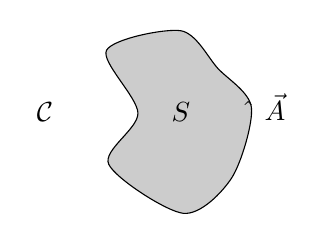
\begin{tikzpicture}
	\draw[->,fill=lightGray] plot [smooth cycle, samples=8,domain={1:8}] (\x*360/8+5*rnd:0.5cm+1cm*rnd) node[right,xshift=-0.25cm] {\^{} $\vec{A}$};
	\node[left] at (-1.5,0) {$\mathcal{C}$};
	\node at (0,0) {$S$};
\end{tikzpicture}
\end{center}
\newpage
Define $\vec{A}_{n}(\vec{R})=i\mel{n,t}{\vec{\nabla}_{R}}{n,t}$ as the \ul{Berry connection vector}.\\

Since $\mathcal{C}$ is a closed curve, $\gamma_{n}(\mathcal{C})=\oint_{\mathcal{C}}\vec{A}_{n}(\vec{R})\cdot\dd{\vec{R}}$ defines the circulation of $\vec{A}$ around the path $\mathcal{C}$. By Stoke's theorem, this can be rewritten as
\begin{equation}
\gamma_{n}=\int_{S}\qty(\vec{\nabla}_{R}\times\vec{A}_{n}(\vec{R}))\cdot\dd{\vec{a}}
\end{equation}
where the integral is over the surface $S$ bounded by path $\mathcal{C}$. We define $\vec{\Omega}_{n}(\vec{R})=\vec{\nabla}_{R}\times\vec{A}_{n}(\vec{R})$ as the \ul{Berry curvature}.\\

Thus, $\gamma_{n}(\mathcal{C})=\int_{S}\vec{\Omega}_{n}(\vec{R})\cdot\dd{\vec{a}}$ is the flux of the Berry curvature through the surface bounded by path $\mathcal{C}$. Thus, $\gamma_{n}(\mathcal{C})$ is non-zero if $\vec{\Omega}_{n}(\vec{R})$ is non-zero. Otherwise, if $\vec{\Omega}_{n}(\vec{R})$ is zero, then the Berry connection vector has no physical consequence and the Berry phase $\gamma_{n}(\vec{R})$ is zero.

\begin{equation}
\vb{H}(\vec{R})\ket*{n(\vec{R})}=E_{n}(\vec{R})\ket*{n(\vec{R})}
\end{equation}
Suppose $\ket*{n(\vec{R})}$ is transformed to $e^{i\Chi(\vec{R})}\ket*{n(\vec{R})}$. The same equation is still satisfied.

\begin{equation}
\vec{\nabla}_{R}\qty(e^{i\Chi(\vec{R})}\ket*{n(\vec{R})})=i\vec{\nabla}_{R}\Chi e^{i\Chi(\vec{R})}\ket*{n(\vec{R})}+e^{i\Chi(\vec{R})}\vec{\nabla}_{R}\ket*{n(\vec{R})}
\end{equation}
Thus, $\vec{A}(\vec{R})$ has been transformed to $\vec{A}(\vec{R})\cdot\vec{\nabla}_{R}\Chi$.\\

Can we always choose $\vec{\nabla}_{R}\Chi=\vec{A}_{n}(\vec{R})$ such that the new $\vec{A}_{n}(\vec{R})$ is zero, such that $\gamma_{n}(\vec{R})=0$? NO! This is only true ($\vec{\nabla}_{R}\Chi=\vec{A}_{n}(\vec{R})$) if $\vec{\nabla}_{R}\times\vec{A}(\vec{R})=\vec{0}$. When $\vec{\Omega}_{n}(\vec{R})\neq\vec{0}$, the phase $\gamma_{n}$ cannot be eliminate by gauge transformation and has observable consequnces. This is analogous to the magnetic field (not in real space, but in the parameter $\vec{R}$).

\subsection{Time-Dependent Perturbation Theory}
The two previous examples are some of the few problems that can be solved analytically. In most cases though, this is not true. As such, we introduce time-dependent perturbation theory for small perturbations to obtain approximate solutions.
\begin{equation}
\vb{H}(t)=\vb{H}_{0}+V(t)\qq{where we assume $V(t)$ is small compared to $\vb{H}_{0}$}
\end{equation}
The time-evolution of a state in the interaction picture is given by
\begin{equation}
i\hbar\pdv{t}\ket{\psi,t}_{\trm{I}}=V^{(\trm{I})}(t)\ket{\psi,t}_{\trm{I}}
\end{equation}
We define the time-evolution operator in the interaction picture as
\begin{equation}
\ket{\psi,t}_{\trm{I}}=V^{(I)}(t)\ket{\psi}
\end{equation}
Substituting into the Schr\"{o}dinger equation in the interaction picture, since $\ket{\psi}$ is an arbitrary state
\begin{equation}
i\hbar\pdv{t}U^{(\trm{I})}(t)=V^{(\trm{I})}(t)U^{(\trm{I})}(t)
\end{equation}
This can be solved formally as
\begin{equation}
U^{(\trm{I})}(t)=\mathbb{I}-\frac{i}{\hbar}\int_{0}^{t}V^{(\trm{I})}(t')U^{(\trm{I})}(t')\dd{t'}
\end{equation}
while subject to the initial condition $U^{(\trm{I})}(0)=\mathbb{I}$.\\

Solving for $U^{(\trm{I})}(t)$ by iteration (where we will drop the (I) superscript for convenience)
\begin{equation}
\begin{aligned}
U(t)&=\mathbb{I}-\frac{i}{\hbar}\int_{0}^{t}\dd{t'}V(t')\qq{(first order approximation)}\\
U(t)&=\mathbb{I}-\frac{i}{\hbar}\int_{0}^{t}\dd{t'}V(t')\qty[\mathbb{I}-\frac{i}{\hbar}\int_{0}^{t'}\dd{t''}V(t'')]\qq{(second order approximation)}\\
&=\mathbb{I}-\frac{i}{\hbar}\int_{0}^{t}\dd{t'}V(t')+\qty(-\frac{i}{\hbar})^{2}\int_{0}^{t}\dd{t'}\int_{0}^{t'}\dd{t''}V(t')V(t'')\\
&\vdots\\
U(t)&=\mathbb{I}-\frac{i}{\hbar}\int_{0}^{t}\dd{t'}V(t')+\qty(-\frac{i}{\hbar})^{2}\int_{0}^{t}\dd{t'}\int_{0}^{t'}\dd{t''}V(t')V(t'')+\ldots\\
&\quad+\qty(-\frac{i}{\hbar})^{n}\int_{0}^{t}\dd{t'}\int_{0}^{t'}\dd{t''}\ldots\int_{0}^{t^{(n-1)}}\dd{t^{(n)}}V(t')V(t'')\ldots V(t^{(n)})\\
&\qq{($n$-th order approximation)}
\end{aligned}
\end{equation}
This series is called the \ul{Dyson series}.\\

Solving the Dyson series is often impossible or impractical. Instead, one can use the Dyson series to calculate the lower-order corrections of the coefficients to get an approximation. Connecting this to the coefficients $c_{n}(t)$
\begin{equation}
\begin{aligned}
\ket{\psi,t}_{\trm{I}}=\sum_{n}c_{n}(t)\ket{n}&=U^{(\trm{I})}(t)\ket{\psi}\\
\sum_{n}c_{n}(t)\ket{n}&=\sum_{n}\op{n}U^{(\trm{I})}(t)\ket{\psi}\qq{by resolution of identity}\\
c_{n}(t)&=\mel{n}{U^{(\trm{I})}(t)}{\psi}
\end{aligned}
\end{equation}
Since $U(t)=\mathbb{I}+\ldots+\qty(-\frac{i}{\hbar})^{n}\int_{0}^{t}\dd{t'}\int_{0}^{t'}\dd{t''}\ldots\int_{0}^{t^{(n-1)}}\dd{t^{(n)}}V(t')V(t'')\ldots V(t^{(n)})$, one can write $c_{n}(t)$ as a series, namely
\begin{equation}
c_{n}(t)=c_{n}^{(0)}+c_{n}^{(1)}(t)+c_{n}^{(2)}(t)+\ldots
\end{equation}
where $c_{n}^{(i)}(t)$ is $c_{n}(t)$ to the $i$-th order of $V^{(\trm{I})}(t)$.
\begin{equation}
\begin{aligned}
c_{n}(t)&=\mel{n}{U^{(\trm{I})}(t)}{\psi}\\
&=\ip{n}{\psi}+\ldots+\qty(-\frac{i}{\hbar})^{n}\int_{0}^{t}\dd{t'}\int_{0}^{t'}\dd{t''}\ldots\int_{0}^{t^{(n-1)}}\mel{n}{V(t')V(t'')\ldots V(t^{(n)})}{\psi}\\
\implies c_{n}^{(n)}(t)&=\qty(-\frac{i}{\hbar})^{n}\int_{0}^{t}\dd{t'}\int_{0}^{t'}\dd{t''}\ldots\int_{0}^{t^{(n-1)}}\dd{t^{(n)}}\mel{n}{V(t')V(t'')\ldots V(t^{(n)})}{\psi}
\end{aligned}
\end{equation}
Let us consider the case where the initial state $\ket{\psi}$ is the energy eigenstate $\ket{i}$, where $\vb{H}_{0}\ket{i}=E_{i}\ket{i}$.
\begin{equation}
\begin{aligned}
c_{n}^{(0)}&=\delta_{ni}\\
c_{n}^{(1)}(t)&=\qty(-\frac{i}{\hbar})\int_{0}^{t}\mel{n}{V^{(\trm{I})}(t')}{o}\dd{t'}\\
&=\qty(-\frac{i}{\hbar})\int_{0}^{t}\mel{n}{e^{\frac{i}{\hbar}\vb{H}_{0}t'}V(t')e^{-\frac{i}{\hbar}\vb{H}_{0}t'}}{i}\dd{t'}\\
&=\qty(-\frac{i}{\hbar})\int_{0}^{t}e^{\frac{i}{\hbar}(E_{n}-E_{i})t'}\mel{n}{V(t')}{i}\dd{t'}\\
&=\qty(-\frac{i}{\hbar})\int_{0}^{t}e^{i\omega_{ni}t'}V_{ni}(t')\dd{t'}\\
&\quad\explain{$\omega_{ni}=\frac{E_{n}-E_{i}}{\hbar}$, $V_{ni}(t)=\mel{n}{V(t)}{i}$}\\
c_{n}^{(2)}(t)&=\qty(-\frac{i}{\hbar})^{2}\int_{0}^{t}\dd{t'}\int_{0}^{t'}\dd{t''}\mel{n}{V^{(\trm{I})}(t')V^{(\trm{I})}(t'')}{i}\\
&=\qty(-\frac{i}{\hbar})^{2}\int_{0}^{t}\dd{t'}\int_{0}^{t'}\dd{t''}\sum_{m}\mel{n}{V^{(\trm{I})}(t')}{m}\mel{m}{V^{(\trm{I})}t'')}{i}\\
&=\qty(-\frac{i}{\hbar})^{2}\int_{0}^{t}\dd{t'}\int_{0}^{t'}\dd{t''}\sum_{m}\mel{n}{V^{(\trm{I})}(t')}{m}\mel{m}{V^{(\trm{I})}(t'')}{i}\\
&=\qty(-\frac{i}{\hbar})^{2}\int_{0}^{t}\dd{t'}\int_{0}^{t'}\dd{t''}\sum_{m}e^{i\omega_{nm}t'}e^{i\omega_{mi}t''}V_{nm}(t')V_{mi}(t'')
\end{aligned}
\end{equation}
In this way, the coefficients $c_{n}(t)$ can be calculated to any order.\\

\aside{The order of $V^{(\trm{I})}(t)$ is important since in general $\comm{V^{(\trm{I})}(t)}{V^{(\trm{I})}(t')}\neq0$ for $t\neq t'$. Consider for example $V(t)=B_{x}\cos(\omega t)\vb{S}_{x}+B_{y}\sin(\omega t)\vb{S}_{y}$.}

One can define a \ul{transition probability} as the probability to find the system in state $\ket{n}$ at time $t$ if the system initially started out in state $\ket{i}$ at time $t=0$.
\begin{equation}
P(i\rightarrow n)=\abs{c_{n}^{(0)}(t)+c_{n}^{(1)}(t)+c_{n}^{(2)}(t)+\ldots}^{2}
\end{equation}
Restricting ourselves to first-order perturbation theory
\begin{equation}
\begin{aligned}
c_{n}^{(1)}(t)&=-\frac{i}{\hbar}\int_{0}^{t}\dd{t'}e^{i\omega_{ni}t'}V_{ni}(t')\\
P(i\rightarrow n)&=\abs{c_{n}^{(0)}(t)+c_{n}^{(1)}(t)}^{2}\\
&=\abs{c_{n}^{(1)}(t)}^{2}\qq{for $n\neq i$}\\
&=\frac{1}{\hbar^{2}}\abs{\int_{0}^{t}e^{i\omega_{ni}t'}V_{ni}(t')}^{2}
\end{aligned}
\end{equation}

Consider the specific example of harmonic perturbation.
\begin{equation}
V(t)=Ve^{i\omega t}+V^{\dagger}e^{-i\omega t}
\end{equation}
where
\begin{equation}
V=\gamma\op{1}{2},\quad V^{\dagger}=\gamma\op{2}{1}
\end{equation}
in the case of the two-level system previously.
\begin{equation}
\begin{aligned}
c_{n}^{(1)}(t)&=-\frac{i}{\hbar}\int_{0}^{t}\dd{t'}e^{i\omega_{ni}t'}V_{ni}(t')\\
&=-\frac{i}{\hbar}\int_{0}^{t}\dd{t'}e^{i\omega_{ni}t'}\qty[V_{ni}e^{i\omega t'}+V_{ni}^{\dagger}e^{-i\omega t'}]\\
&=\qty(-\frac{i}{\hbar})\qty[\frac{V_{ni}\qty(e^{i(\omega_{ni}+\omega)t}-1)}{i(\omega_{ni}+\omega)}+\frac{V_{ni}^{\dagger}\qty(e^{i(\omega_{ni}-\omega)t}-1)}{i(\omega_{ni}-\omega)}]\\
&=\frac{1}{\hbar}\qty[\frac{V_{ni}\qty(1-e^{i(\omega_{ni}+\omega)t})}{(\omega_{ni}+\omega)}+\frac{\qty(1-e^{i(\omega_{ni}-\omega)t})V_{in}^{*}}{(\omega_{ni}-\omega)}]
\end{aligned}
\end{equation}
The transition probability will only be significant if the resonance condition is satisfied (i.e. $\omega\approx\pm\omega_{ni}$). More specifically, $c_{n}^{(1)}(t)$ becomes maximized. Assume $\omega\approx\omega_{ni}$. Thus, the second term dominates in $c_{n}^{(1)}(t)$. Therefore
\begin{equation}
\begin{aligned}
c_{n}^{(1)}(t)&\approx\qty(\frac{1}{\hbar})\qty[\frac{(1-e^{i(\omega_{ni}-\omega)t})V_{in}^{*}}{(\omega_{ni}-\omega)}]\\
\implies \abs{c_{n}^{(1)}(t)}^{2}&=\frac{\abs{V_{in}}^{2}}{\hbar^{2}}\abs{\frac{1-e^{i(\omega_{ni}-\omega)t}}{\omega_{ni}-\omega}}^{2}\\
&=\frac{\abs{V_{in}}^{2}}{\hbar^{2}}\frac{\qty(1-e^{i(\omega_{ni}-\omega)t})\qty(1-e^{-i(\omega_{ni}-\omega)t})}{(\omega_{ni}-\omega)^{2}}\\
&=\frac{\abs{V_{in}}^{2}}{\hbar^{2}(\omega_{ni}-\omega)^{2}}\qty[1+1-2\cos\qty(\qty(\omega_{ni}-\omega)t)]\\
&=\frac{2\abs{V_{in}}^{2}}{\hbar^{2}(\omega_{ni}-\omega)^{2}}\qty[1-\cos\qty(\qty(\omega_{ni}-\omega)t)]\\
&=\frac{4\abs{V_{in}}^{2}}{\hbar^{2}(\omega_{ni}-\omega)^{2}}\sin^{2}\qty(\frac{(\omega_{ni}-\omega)t}{2})\\
&=\frac{\abs{V_{in}}^{2}}{\hbar^{2}}\frac{\sin^{2}\qty(\frac{(\omega_{ni}-\omega)t}{2})t^{2}}{\qty(\frac{(\omega_{ni}-\omega)t}{2})^{2}}\\
&=P(i\rightarrow n)
\end{aligned}
\end{equation}
Let us consider the probability in its long-term behaviour (i.e. $t\rightarrow\infty$). Note however that the time-dependent perturbation becomes less and less valid at later times. As such, one qualifies this analysis by saying that one looks at large times, but not too large that the perturbation breaks down. Let $\alpha=\frac{\omega_{ni}-\omega}{2}$.
\begin{equation}
f(\alpha)=\lim_{t\rightarrow\infty}\frac{\sin^{2}(\alpha t)}{\pi\alpha^{2}t}
\end{equation}
When $\alpha\neq0$, $f(\alpha)=0$. However, for $\alpha t\ll 1$, $\sin^{2}(\alpha t)\approx \alpha^{2}t^{2}$.
\begin{equation}
\begin{aligned}
f(0)&=\lim_{t\rightarrow\infty}\lim_{\alpha\rightarrow0}\frac{\sin^{2}(\alpha t)}{\pi\alpha^{2}t}\\
&=\lim_{t\rightarrow\infty}\lim_{\alpha\rightarrow0}\frac{\alpha^{2}t^{2}}{\pi\alpha^{2}t}\\
&=\lim_{t\rightarrow\infty}\frac{t}{\pi}\\
&=\infty
\end{aligned}
\end{equation}
Note also that
\begin{equation}
\begin{aligned}
\int_{-\infty}^{\infty}\dd{\alpha}f(\alpha)&=\int_{-\infty}^{\infty}\frac{\sin^{2}(\alpha t)}{\pi\alpha^{2}t}=1
\therefore f(\alpha)&=\delta(\alpha)
\end{aligned}
\end{equation}
Note that the factor of $\pi$ makes $f(a)=\delta(\alpha)$ exactly.\\

Consider the transition rate for transition probability per unit time
\begin{equation}
W(i\rightarrow n)=\dv{t}P(i\rightarrow n)
\end{equation}
At $t=\infty$
\begin{equation}
\begin{aligned}
P(i\rightarrow n)&=\lim_{t\rightarrow\infty}\frac{\pi\abs{V_{in}}^{2}}{\hbar^{2}}\delta\qty(\frac{\omega_{ni}-\omega}{2})t\\
&=\lim_{t\rightarrow\infty}\frac{2\pi\abs{V_{in}}^{2}}{\hbar^{2}}\delta(E_{n}-E_{i}-\hbar\omega)t\qq{since $\delta(cx)=\frac{1}{\abs{c}}\delta(x)$}\\
W(i\rightarrow n)&=\dv{t}P(i\rightarrow n)\\
&=\frac{2\pi\abs{V_{in}}^{2}}{\hbar}\delta(E_{n}-E_{i}-\hbar\omega)
\end{aligned}
\end{equation}
This equation for $W(i\rightarrow n)$ at $t=\infty$ is known as \ul{Fermi's golden rule}. This $\delta$-function expresses energy conservation in the sense that it is only non-zero if $E_{n}-E_{i}=\hbar\omega$. For example, if the final state has a larger energy than the initial state ($E_{n}>E_{i}$), the the only way to transition from $\ket{i}$ to $\ket{n}$ is to absorb a quanta with energy $\hbar\omega=E_{n}-E_{i}$. This is known as \ul{absorption}. In contrast, when $E_{i}>E_{n}$, the only way to transition is to emit a quanta with energy $\hbar\omega=E_{i}-E_{n}$ (equivalent to absorbing a quanta with $-\hbar\omega=E_{n}-E_{i}$). This is called \ul{stimulated emission}.
\begin{center}
\begin{tikzpicture}
	\draw (0,0) node[left] {$E_{i}$} -- (3,0);
	\draw (0,2) node[left] {$E_{n}$} -- (3,2);
	\draw[->,thick] (1,0) -- node[right] {$\hbar\omega=E_{n}-E_{i}$} (1,2);
	\node[anchor=north west,right] at (5,1)
		{\[
			\begin{aligned}
				&\trm{For absorption}\\
				&W(i\rightarrow n)=\dv{P(i\rightarrow n)}{t}=\frac{2\pi\abs{V_{in}}^{2}}{\hbar}\delta(E_{n}-E_{i}-\hbar\omega)
			\end{aligned}
		\]};
\end{tikzpicture}
\end{center}

\begin{center}
\begin{tikzpicture}
	\draw (0,0) node[left] {$E_{n}$} -- (3,0);
	\draw (0,2) node[left] {$E_{i}$} -- (3,2);
	\draw[<-,thick] (1,0) -- node[right] {$\hbar\omega=E_{n}-E_{i}$} (1,2);
	\node[anchor=north west,right] at (5,1)
		{\[
			\begin{aligned}
				&\trm{For stimulated emission}\\
				&W(i\rightarrow n)=\dv{P(i\rightarrow n)}{t}=\frac{2\pi\abs{V_{in}}^{2}}{\hbar}\delta(E_{n}-E_{i}+\hbar\omega)
			\end{aligned}
		\]};
\end{tikzpicture}
\end{center}
The probability under a time-independent (constant) perturbation can be computed by setting $\omega=0$.
\begin{equation}
\therefore\abs{c_{n}^{(1)}(t)}^{2}=\frac{\abs{V_{in}}^{2}}{\hbar^{2}}\frac{\sin^{2}\qty(\frac{\omega_{ni}t}{2})}{\qty(\frac{\omega_{ni}}{2})^{2}}
\end{equation}
Plotting $f(\omega_{ni})=\frac{\sin^{2}\qty(\frac{\omega_{ni}t}{2})}{\qty(\frac{\omega_{ni}}{2})^{2}}$
\begin{center}
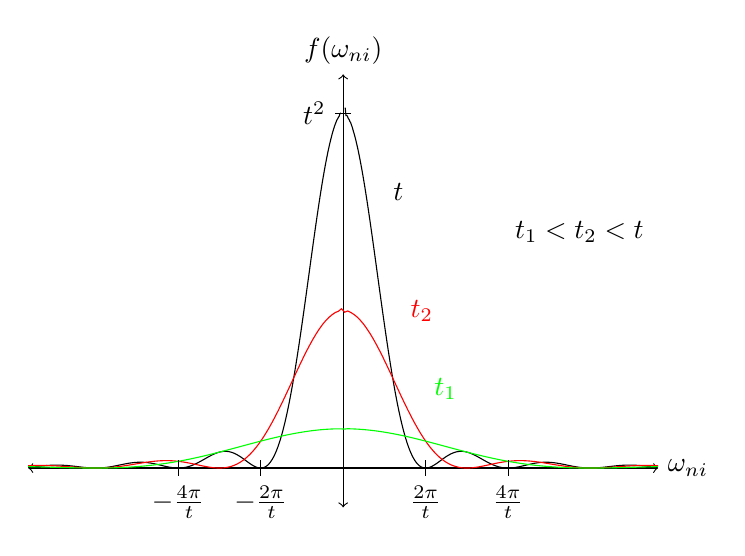
\begin{tikzpicture}
	\draw[<->] (-4,0) -- (4,0) node[right] {$\omega_{ni}$};
	\draw[<->] (0,-0.5) -- (0,5) node[above] {$f(\omega_{ni})$};
	\draw[domain=-4:-0.025,samples=400] plot (\x, {0.5*(sin(deg(3*\x)))^2/(\x)^2});
	\draw[domain=0.025:4,samples=400] plot (\x, {0.5*(sin(deg(3*\x)))^2/(\x)^2});
	\draw[domain=-4:4,samples=200,red] plot (\x, {0.5*(sin(deg(2*\x)))^2/(\x)^2});
	\draw[domain=-4:4,samples=200,green] plot (\x, {0.5*(sin(deg(\x)))^2/(\x)^2});
	\draw (0.1,4.5) -- (-0.1,4.5) node[left] {$t^{2}$};
	\draw (-2.094,0.1) -- (-2.094,-0.1) node[below] {$-\frac{4\pi}{t}$};
	\draw (-1.047,0.1) -- (-1.047,-0.1) node[below] {$-\frac{2\pi}{t}$};
	\draw (1.047,0.1) -- (1.047,-0.1) node[below] {$\frac{2\pi}{t}$};
	\draw (2.094,0.1) -- (2.094,-0.1) node[below] {$\frac{4\pi}{t}$};
	\node at (0.7,3.5) {$t$};
	\node[red] at (1,2) {$t_{2}$};
	\node[green] at (1.3,1) {$t_{1}$};
	\node at (3,3) {$t_{1}<t_{2}<t$};
\end{tikzpicture}
\end{center}
At $\omega_{ni}=0$
\begin{equation}
f(0)=\lim_{\omega_{ni}\rightarrow0}\frac{\sin^{2}\qty(\frac{\omega_{ni}t}{2})}{\qty(\frac{\omega_{ni}}{2})^{2}}=t^{2}
\end{equation}
As time increases the height of the central peak increases as $t^{2}$, while its width decreases as $\frac{1}{t}$. At long times, $P(i\rightarrow n)$ becomes appreciable only for states with
\begin{equation}
\begin{aligned}
\abs{\omega_{ni}}&\sim\frac{2\pi}{t}\\
\implies\abs{\frac{E_{n}-E_{i}}{\hbar}}&\sim\frac{2\pi}{t}\\
\abs{E_{n}-E_{i}}t&\sim2\pi\hbar
\end{aligned}
\end{equation}
This is similar to the energy-time uncertainty relation $\Delta E\Delta t\sim\hbar$.\\

Consider now the initial state $\ket{i}$ under the action of the perturbation. It is convenient to use a gradually turned on perturbation of the form
\begin{equation}
V(t)=Ve^{\eta t},\,\eta>0,\,\eta\rightarrow0^{+}
\end{equation}
Confirming that we get the same results as before, for $n\neq i$
\begin{equation}
\begin{aligned}
c_{n}^{(1)}(t)&=-\frac{i}{\hbar}V_{ni}\int_{-\infty}^{t}\dd{t'}e^{\eta t'}e^{i\omega_{ni}t'}\\
&\quad\explain{The lower bound is negative infinity as for any finite $\eta>0$, $V(t\rightarrow-\infty)=0$. The perturbation is absent at $t\rightarrow-\infty$ and is slowly turned on.}\\
&=-\frac{i}{\hbar}V_{ni}\qty(\frac{e^{\eta t+i\omega_{ni}t}}{\eta+i\omega_{ni}})\\
\abs{c_{n}^{(1)}(t)}^{2}&=\frac{\abs{V_{ni}}^{2}}{\hbar^{2}}\frac{e^{2\eta t}}{\eta^{2}+\omega_{ni}^{2}}=P(i\rightarrow n)
\end{aligned}
\end{equation}
Thus
\begin{equation}
\begin{aligned}
W(i\rightarrow n)&=\dv{t}\abs{c_{n}^{(1)}(t)}^{2}\\
&=\frac{2\abs{V_{in}}^{2}}{\hbar^{2}}\frac{\eta e^{2\eta t}}{\eta^{2}+\omega_{ni}^{2}}
\end{aligned}
\end{equation}
Note that
\begin{equation}
\begin{aligned}
\lim_{\eta\rightarrow 0}\frac{\eta}{\eta^{2}+\omega_{ni}^{2}}=\pi\delta(\omega_{ni}=\pi\hbar\delta(E_{n}-E_{i})
\end{aligned}
\end{equation}
since
\begin{equation}
\lim_{\eta\rightarrow0}\frac{\eta}{\eta^{2}+\omega_{ni}^{2}}=\begin{cases}
0 & \trm{if $\omega_{ni}\neq0$}\\
\infty & \trm{if $\omega_{ni}=0$}
\end{cases}
\end{equation}
and
\begin{equation}
\int_{-\infty}^{\infty}\dd{\omega_{ni}}\frac{\eta}{\eta^{2}+\omega_{ni}^{2}}=\pi
\end{equation}
\newpage
Through this, one calculates the probability that the system remains in state $\ket{i}$.
\begin{equation}
\begin{aligned}
c_{i}^{(0)}(t)&=1\\
c_{i}^{(1)}(t)&=\qty(-\frac{i}{\hbar})V_{ii}\int_{-\infty}^{t}\dd{t'}e^{\eta t'}e^{i\omega_{ii}t'}\\
&=\qty(-\frac{i}{\hbar\eta})V_{ii}e^{\eta t}\qq{since $\omega_{ii}=0$}\\
c_{i}^{(2)}(t)&=\qty(-\frac{i}{\hbar})^{2}\sum_{m}\int_{-\infty}^{t}\dd{t'}\int_{-\infty}^{t'}\int_{-\infty}^{t'}\dd{t''}e^{i\omega_{im}t'}e^{i\omega_{mi}t''}V_{im}(t')V_{mi}(t'')\\
&=\qty(-\frac{i}{\hbar})^{2}\sum_{m}\abs{V_{mi}}^{2}\int_{-\infty}^{t}\dd{t'}\int_{-\infty}^{t'}\dd{t''}e^{\eta t'}e^{i\omega_{im}t'}e^{\eta t''}e^{i\omega_{mi}t''}\\
&=\qty(-\frac{i}{\hbar})^{2}\sum_{m}\abs{V_{mi}}^{2}\int_{-\infty}^{t}\dd{t'}e^{\eta t'}e^{i\omega_{im}t'}\qty(\frac{e^{\eta t'}e^{i\omega_mi}t'}{\eta+i\omega_{mi}})\\
&=\qty(-\frac{i}{\hbar})^{2}\sum_{m}\abs{V_{mi}}^{2}\frac{e^{2\eta t}}{2\eta(\eta+i\omega_{mi})}\\
&=\qty(-\frac{i}{\hbar})^{2}\abs{V_{ii}}^{2}\frac{e^{2\eta t}}{2\eta^{2}}+\qty(-\frac{i}{\hbar})^{2}\sum_{m\neq i}\abs{V_{mi}}^{2}\frac{e^{2\eta t}}{2\eta\qty(\eta+i\frac{E_{m}-E_{i}}{\hbar})}\\
&=\qty(-\frac{i}{\hbar})^{2}\abs{V_{ii}}^{2}\frac{e^{2\eta t}}{2\eta^{2}}+\qty(-\frac{i}{\hbar})\sum_{m\neq i}\abs{V_{mi}}^{2}\frac{e^{2\eta t}}{2\eta(E_{i}-E_{m}+i\hbar\eta)}
\end{aligned}
\end{equation}
Thus
\begin{equation}
\begin{aligned}
c_{i}(t)&\approx c_{i}^{(0)}(t)+c_{i}^{(1)}(t)+c_{i}^{(2)}(t)\\
&=1-\frac{i}{\hbar\eta}V_{ii}V^{\eta t}+\qty(-\frac{i}{\hbar})^{2}\abs{V_{ii}}^{2}\frac{e^{2\eta t}}{2\eta^{2}}+\qty(-\frac{i}{\hbar})\sum_{m\neq i}\abs{V_{mi}}^{2}\frac{e^{2\eta t}}{2\eta(E_{i}-E_{m}+i\hbar\eta)}
\end{aligned}
\end{equation}
and
\begin{equation}
\hspace{-1cm}
\begin{aligned}
\frac{1}{c_{i}(t)}\dv{c_{i}(t)}{t}&=\frac{-\frac{i}{\hbar}V_{ii}e^{\eta t}+\qty(-\frac{i}{\hbar})^{2}\abs{V_{ii}}^{2}\frac{e^{2\eta t}}{\eta}+\qty(-\frac{i}{\hbar})\sum_{m\neq i}\abs{V_{mi}}^{2}\frac{e^{2\eta t}}{E_{i}-E_{m}+i\hbar\eta}}{1-\frac{i}{\hbar\eta}V_{ii}e^{\eta t}}\\
&=\qty[\qty(-\frac{i}{\hbar})V_{ii}e^{\eta t}+\qty(-\frac{i}{\hbar})^{2}\abs{V_{ii}}^{2}\frac{e^{2\eta t}}{\eta}+\qty(-\frac{i}{\hbar})^{2}\sum_{m\neq i}\abs{V_{im}}^{2}\frac{e^{2\eta t}}{E_{i}-E_{m}+i\hbar\eta}]\qty[1+\frac{i}{\hbar}V_{ii}\frac{e^{\eta t}}{\eta}]\\
&\quad\explain{By binomial approximation, since $\frac{V_{ii}}{\hbar\eta}\ll1$}\\
&\approx-\frac{i}{\hbar}V_{ii}+\qty(-\frac{i}{\hbar})\sum_{m\neq i}\frac{\abs{V_{im}}^{2}}{E_{i}-E_{m}+i\hbar\eta}\\
&\quad\explain{Up to second order in $V$ and using that $\eta\rightarrow0^{+}$}
\end{aligned}
\end{equation}
Defining $\Delta_{i}$ as
\begin{equation}
\begin{aligned}
\Delta_{i}&=V_{ii}+\sum_{m\neq i}\frac{\abs{V_{im}}^{2}}{E_{i}-E_{m}+i\hbar\eta}\\
\implies\dv{c_{i}}{t}&=-\frac{i}{\hbar}\Delta_{i}c_{i}(t)\\
\implies c_{i}(t)&=c_{i}(0)e^{-\frac{i}{\hbar}\Delta_{i}t}\qq{(interaction picture)}\\
&\trm{or}\\
c_{i}(t)&=c_{i}(0)e^{-\frac{i}{\hbar}E_{i}t}e^{-\frac{i}{\hbar}\Delta_{i}t}\qq{($c_{i}(0)=1$ for initial state $\ket{i}$)}
\end{aligned}
\end{equation}
What is the physical meaning of this result? Recall that $c_{i}(t)$ are the coefficients of the wavefunction in the interaction picture. Decomposing the contributions into two orders
\begin{equation}
\begin{aligned}
\Delta_{i}&=\Delta_{i}^{(1)}+\Delta_{i}^{(2)}\\
\implies\Delta_{i}^{(1)}&=V_{ii}\qq{which agrees with first order time-independent perturbation theory}
\end{aligned}
\end{equation}
However
\begin{equation}
\Delta_{i}^{(2)}=\sum_{m\neq i}\abs{V_{im}}^{2}\frac{1}{E_{i}-E_{m}-i\hbar\eta}
\end{equation}
Note that
\begin{equation}
\begin{aligned}
\Im\qty(\frac{1}{\Chi+i\epsilon})&=\Im\qty(\frac{\Chi-i\epsilon}{\Chi^{2}+\epsilon^{2}})\\
&=-\frac{\epsilon}{\Chi^{2}+\epsilon^{2}}\\
&=-\pi\delta(x)\\
\implies \Im(\Delta_{i}^{2})&=-\pi\sum_{m\neq i}\abs{V_{im}}^{2}\delta(E_{i}-E_{m})
\end{aligned}
\end{equation}
In comparison with Fermi's golden rule with $\omega=0$
\begin{equation}
\begin{aligned}
\sum_{m\neq i}W(i\rightarrow m)&=\frac{2\pi}{\hbar}\sum_{m\neq i}\abs{V_{mi}}^{2}\delta(E_{i}-E_{m})\\
&=-\frac{2}{\hbar}\Im(\Delta_{i}^{(2)})
\end{aligned}
\end{equation}
Note that $\ket{\psi,t}_{\trm{I}}=\sum_{n}c_{n}(t)\ket{n}$. Thus, $\Re(\Delta_{i})$ has the meaning of the shift of energy of $\ket{i}$ under the action of the perturbation.\\

Define $\Gamma_{i}=-2\Im(\Delta_{i})>0$ as a decay constant. Then
\begin{equation}
\begin{aligned}
c_{i}(t)&=e^{-\frac{i}{\hbar}\qty(\Re(\Delta_{i})+i\Im(\Delta_{i}))t}\\
\therefore \abs{c_{i}(t)}^{2}&=e^{\frac{2}{\hbar}\Im(\Delta_{i})t}=e^{-\frac{\Gamma_{i}}{\hbar}}=e^{-\frac{t}{\tau_{i}}}
\end{aligned}
\end{equation}
Thus, $\Gamma_{i}$ is the decay rate for state $\ket{i}$ and $\tau_{i}=\frac{\hbar}{\Gamma_{i}}$ is the lifetime of state $\ket{i}$.\\

In the Schr\"{o}dinger picture
\begin{equation}
c_{i}(t)=e^{-\frac{i}{\hbar}E_{i}t}e^{-\frac{1}{2\hbar}\Gamma_{i}t}
\end{equation}
Taking the Fourier transformation with respect to $t$
\begin{equation}
\begin{aligned}
\int_{0}^{\infty}\dd{t}e^{\frac{i}{\hbar}Et}e^{-\frac{i}{\hbar}E_{i}t-\frac{1}{2\hbar}\Gamma_{i}t}&=-\frac{1}{\qty(\frac{i}{\hbar})\qty(E-E_{i}+\frac{i\Gamma_{i}}{2})}=\frac{i\hbar}{\qty(E-E_{i}+\frac{i\Gamma_{i}}{2})}\\
\Im\qty(\frac{1}{E-E_{i}+\frac{i\Gamma_{i}}{2}})&=-\frac{\frac{1}{2}\Gamma_{i}}{(E-E_{1})^{2}+\frac{\Gamma_{i}^{2}}{4}}=A(E)\qq{(spectral function)}\\
\lim_{\Gamma_{i}\rightarrow 0}\frac{\frac{1}{2}\Gamma_{i}}{(E-E_{i})^{2}+\frac{\Gamma_{i}^{2}}{4}}&=\pi\delta(E-E_{i})
\end{aligned}
\end{equation}

\begin{center}
\begin{tikzpicture}
	\draw[<->] (-4,0) -- (4,0) node[right] {$E-E_{i}$};
	\draw[<->] (0,-0.5) -- (0,4.5) node[above] {$A(E)$};
	\draw[domain=-4:4,samples=200] plot (\x, {2/((\x)^2+0.5)});
	\node[right,xshift=0.3cm] at (0,4) {$\frac{1}{\Gamma_{i}}$};
	\draw[<->] (-0.704,2) -- (0.704,2);
	\node[right] at (0.8,2) {$\Delta E=\Gamma_{i}$ at full width half maximum};
\end{tikzpicture}
\end{center}
The width of the peak is $\Gamma_{I}$. One can say that the energy level $E_{i}$ has been broadened by $\Gamma_{i}$ due to the perturbation.
\begin{equation}
\Delta E\sim\Gamma_{i}=\frac{\hbar}{\tau_{i}}
\end{equation}
Thus, $\Delta E\tau_{i}\sim\hbar$, which is another way to view the energy-time uncertainty relation. Moreover, one can see that for $t>\tau_{i}$, the probability to find the system in the initial state becomes exponentially small.

\newpage
\section{Relativistic Quantum Mechanics}
Let us find a generalization of quantum mechanics consistent with special relativity, with which one will use to analyze fast moving particles.\\

There are two main principles of special relativity
\begin{enumerate}
\item The laws of nature are the same in all frames of reference where an inertial frame is a frame in which a free body moves with constant velocity.
\item The speed of light is the same in all inertial frames of reference, with nothing moving faster than this speed.
\end{enumerate}
Let us define an \ul{event} to be something that happens at a specific time and point in space ($\vec{x}$,$t$). Consider two events ($\vec{x}_{1}$,$t_{1}$) and ($\vec{x}_{2}$,$t_{2}$). The \ul{interval} between them is
\begin{equation}
s_{12}=\sqrt{c^{2}(t_{2}-t_{1})^{2}-(\vec{x}_{2}-\vec{x}_{1})^{2}}
\end{equation}
where $c$ is the speed of light. It is measured by the emission of light at ($\vec{x}_{1}$,$t_{1}$) and detection of the same beam of light at ($\vec{x}_{2}$,$t_{2}$).\\

Since light always propagates at the speed of light $c$, one has $\abs{\vec{x}_{2}-\vec{x}_{1}}=c(t_{2}-t_{1})$ such that $s_{12}=0$. This interval is called a \ul{light-like interval}. In general, $s_{12}^{2}$ can also be positive or negative. If $s_{12}^{2}>0$, the two events could in principle be related by a physical signal. This interval is \ul{time-like}. If $s_{12}^{2}<0$, the events are non-related, yielding a \ul{space-like interval}.\\

Consider an infinitesimally small interval
\begin{equation}
\dd{s^{2}}=c^{2}\dd{t^{2}}-\dd{l^{2}}, \quad\dd{l}=\sqrt{\dd{x}^{2}+\dd{y}^{2}+\dd{z}^{2}}
\end{equation}
In another inertial frame
\begin{equation}
\dd{s'{}^{2}}=c^{2}\dd{t'{}^{2}}=c^{2}\dd{t'{}^{2}}-\dd{l'{}^{2}},\quad\dd{l'}=\sqrt{\dd{x'{}^{2}}+\dd{y'{}^{2}}+\dd{z'{}^{2}}}
\end{equation}
By Taylor series
\begin{equation}
\dd{s^{2}}=f(\dd{s'{}^{2}}=a+b\dd{s'{}^{2}}+\cancelto{0}{\order{(\dd{s'{}^{2}})^{2}}}
\end{equation}
For a light-like interval, $\dd{s^{2}}=0$. Thus
\begin{equation}
\dd{s^{2}}=b\dd{s'{}^{2}}\qq{($a$ must equal to 0)}
\end{equation}
Furthermore, $b$ cannot depend on $\vec{x}$ or $t$ as that would violate the uniformity of space and time. Thus
\begin{equation}
b=b(\vec{v})\qq{where $\vec{v}$ is the relative velocity between two frames}
\end{equation}
Also, $b$ cannot depend on the direction of $\vec{v}$ due to the isotropy of space. Thus, $b=b(v)$.\\

Suppose one has three frames $K$, $K'$, and $K''$. The relative velocities are
\begin{itemize}
\item $\vec{v}_{1}$ between $K$ and $K'$
\item $\vec{v}_{2}$ between $K'$ and $K''$
\item $\vec{v}_{3}$ between $K$ and $K''$
\end{itemize}
Thus
\begin{itemize}
\item $\dd{s^{2}}=b(v_{1})\dd{s'{}^{2}}$
\item $\dd{s'{}^{2}}=b(v_{2})\dd{s''{}^{2}}$
\item $\dd{s^{2}}=b(v_{12})\dd{s''{}^{2}}$
\end{itemize}
Thus
\begin{equation}
b(v_{12})=b(v_{1})b(v_{2})
\end{equation}
$v_{12}$ in general depends on the angle between $\vec{v}_{1}$ and $\vec{v}_{2}$. Thus, $v_{12}$ is a function of $v_{1}$, $v_{2}$, and the angle between them. However, $b(v_{1})b(v_{2})$ is simply a product and does not depend on the angle between $\vec{v}_{1}$ and $\vec{v}_{2}$. Thus, $b(v)$ is a constant and must equal to 1, as this must hold true for all $v$. Thus
\begin{equation}
\dd{s^{2}}=\dd{s'{}^{2}}\qq{(Interval is invariant in all reference frames)}
\end{equation}
Transformations between reference frames must preserve the interval.

\subsection{Proper Time}
Consider a particle with velocity $\vec{v}$ in the laboratory frame.
\begin{equation}
v=\dv{l}{t},\quad\dd{l}=\sqrt{\dd{x}^{2}+\dd{y}^{2}+\dd{z}^{2}}
\end{equation}
where $\dd{l}$ is the distance moved in the lab frame in time $\dd{t}$. Recall that
\begin{equation}
\dd{s}^{2}=c^{2}\dd{t}^{2}-\dd{l}^{2}
\end{equation}
In the frame where the particle is at rest
\begin{equation}
\dd{l'{}^{2}}=0\implies \dd{s'{}^{2}}=c^{2}\dd{t'{}^{2}}
\end{equation}
Since $\dd{s^{2}}=\dd{s'{}^{2}}$
\begin{equation}
\begin{aligned}
c^{2}\dd{t^{2}}-\dd{l^{2}}&=c^{2}\dd{t'{}^{2}}\\
\dd{t'}&=\sqrt{\dd{t^{2}}-\frac{\dd{l^{2}}}{c^{2}}}\\
&=\dd{t}\sqrt{1-\frac{1}{c^{2}}\frac{\dd{l^{2}}}{\dd{t^{2}}}}\\
&=\dd{t}\sqrt{1-\frac{v^{2}}{c^{2}}}
\end{aligned}
\end{equation}

$\dd{t'}$ is denoted the \ul{proper time interval}, which is taken in the frame of the moving particle.

\subsection{4-Vectors}
Let us define the \ul{contravariant 4-position} as
\begin{equation}
x^{\mu}=(x^{0},x^{1},x^{2},x^{3})=(ct,x,y,z)
\end{equation}
Let us also define the \ul{covariant 4-position} as
\begin{equation}
x_{\mu}=(ct,-x,-y,-z)
\end{equation}
The scalar product of the 4-vectors yields the invariant interval
\begin{equation}
x^{\mu}x_{\mu}=c^{2}t^{2}-x^{2}-y^{2}-z^{2}=ct^{2}-\abs*{\vec{x}}^{2}\qq{(Lorentz scalar)}
\end{equation}
This interval is invariant with respect to Lorentz transformations such as rotations and reference frame transformations.
\begin{equation}
\dd{x^{\mu}}=(c\dd{t},\dd{x},\dd{y},\dd{z})
\end{equation}
The \ul{4-velocity} is
\begin{equation}
\begin{aligned}
u^{\mu}&=\dv{x^{\mu}}{s}=\frac{1}{c}\dv{x^{\mu}}{t_{\trm{proper}}}=\frac{1}{c\sqrt{1-\frac{v^{2}}{c^{2}}}}\dv{x^{\mu}}{t}=\qty(\frac{1}{\sqrt{1-\frac{v^{2}}{c^{2}}}},\frac{\vec{v}}{c\sqrt{1-\frac{v^{2}}{c^{2}}}})\\
u^{\mu}u_{\mu}&=\frac{1}{1-\frac{v^{2}}{c^{2}}}-\frac{\frac{v^{2}}{c^{2}}}{1-\frac{v^{2}}{c^{2}}}=1\qq{(invariant under transformations)}
\end{aligned}
\end{equation}
Note that one uses $\dd{s}$ instead of $\dd{t}$ as $\dd{t}$ changes with changes of reference frame.\\

The \ul{4-momentum} is
\begin{equation}
p^{\mu}=mcu^{\mu}=\qty(\frac{mc}{\sqrt{1-\frac{v^{2}}{c^{2}}}},\frac{m\vec{v}}{\sqrt{1-\frac{v^{2}}{c^{2}}}})=\qty(\frac{E}{c},\vec{p})
\end{equation}
where $m$ is the rest mass. Note the extra factor of $\frac{1}{\sqrt{1-\frac{v^{2}}{c^{2}}}}$ for relativistic energy and momentum.
\begin{equation}
\begin{aligned}
p^{\mu}p_{\mu}&=\frac{E^{2}}{c^{2}}-\abs*{\vec{p}}^{2}=\frac{m^{2}c^{2}}{1-\frac{v^{2}}{c^{2}}}-\frac{m^{2}v^{2}}{1-\frac{v^{2}}{c^{2}}}=m^{2}c^{2}\qq{(invariant under transformation)}\\
\implies E^{2}&=m^{2}c^{4}+\abs*{\vec{p}}^{2}c^{2}
\end{aligned}
\end{equation}
Using natural units ($\hbar=c=1$) that are often employed in relativistic quantum mechanics
\begin{equation}
E^{2}=m^{2}+\abs*{\vec{p}}^{2}
\end{equation}
Furthermore, in natural units
\begin{equation}
\vec{p}=-i\vec{\nabla}\qq{and}E=\vb{H}=i\pdv{t}
\end{equation}
where previously $\vec{p}=-i\hbar\vec{\nabla}$ and $\vb{H}=i\hbar\pdv{t}$. The Schr\"{o}dinger equation in natural units is $i\pdv{t}\psi(\vec{x},t)=-\frac{\vec{\nabla}^{2}}{2m}\psi(\vec{x},t)$. Note the Schr\"{o}dinger equation is not invariant under Lorentz transformations.

\subsection{Free Relativistic Particle}
Consider a free particle. In non-relativistic quantum mechanics, $E=\vb{H}=\frac{\vec{p}^{2}}{2m}$. This yields the Schr\"{o}dinger equation
\begin{equation}
i\pdv{t}\psi=-\frac{\vec{\nabla}^{2}}{2m}\psi
\end{equation}
For a relativistic particle, $E=\sqrt{m^{2}+\vec{\vb{p}}^{2}}$. Thus
\begin{equation}
i\pdv{t}\psi=\sqrt{m^{2}-\vec{\nabla}^{2}}\psi
\end{equation}
This is a bad equation as the right-hand side is highly non-local. It contains an infinite series of derivatives, as can be seen by Taylor expanding the expression for $E$. It becomes impossible to formulate a ``covariant" wave equation.\\

Instead, taking the square $E^{2}=m^{2}+\vec{\vb{p}}^{2}$
\begin{equation}
\begin{aligned}
-\pdv[2]{t}\psi(\vec{x},t)&=(m^{2}-\vec{\nabla}^{2})\psi(\vec{x},t)\\
\therefore\qty(\pdv[2][{t}-\vec{\nabla}^{2}+m^{2})\psi(\vec{x},t)&=0
\end{aligned}
\end{equation}
This is the \ul{Klein-Gordon equation}. Note this equation has some problems. It permits solutions with negative energy. Likewise, a second order time derivative can not be defined from the time-evolution operator.\\

In relativistic notation, if $F(x^{\mu})$ is a scalar
\begin{equation}
\begin{aligned}
\dd{F}&=\pdv{F}{x^{\mu}}\dd{x^{\mu}}\\
\therefore\pdv{x^{\mu}}&=\qty(\pdv{t},\vec{\nabla})
\end{aligned}
\end{equation}
We define $\partial_{\mu}=\qty(\pdv{t},\vec{\nabla})$ as the \ul{covariant 4-gradient} and $\partial^{\mu}=\qty(\pdv{t},-\vec{\nabla})$ as the \ul{contravariant 4-gradient}. Note the opposite signs from regular 4-vectors.
\begin{equation}
\pd{\mu}\pu{\mu}=\pu{\mu}\pd{\mu}=\pdv[2]{t}-\vec{\nabla}^{2}
\end{equation}
The Klein-Gordon equation becomes
\begin{equation}
\qty(\pd{\mu}\pu{\mu}+m^{2})\psi=0
\end{equation}
This is clearly Lorentz invariant, as $\pd{\mu}\pu{\mu}$ is a Lorentz scalar and $m^{2}$ is a constant.\\

One expects the solution to this equation to have the ansatz form of a plane-wave
\begin{equation}
\psi(\vec{x},t)=Ne^{i(\vec{p}\cdot\vec{x}-Et)}=Ne^{-ip^{\mu}x_{\mu}}
\end{equation}
where $p^{\mu}=(E,\vec{p})$ and $x_{\mu}=(t,-\vec{x})$.\\

Checking to see if the equation is satisfied
\begin{equation}
\begin{aligned}
\qty(\pdv[2]{t}-\vec{\nabla}^{2}+m^{2})\psi(\vec{x},t)&=\qty(\pdv[2]{t}-\vec{\nabla}^{2}+m^{2})Ne^{i(\vec{p}\cdot\vec{x}-Et)}\\
&=(-E^{2}+\vec{p}^{2}+m^{2})\psi(\vec{x},t)\\
&=0
\end{aligned}
\end{equation}
Since $\psi(\vec{x},t)\neq0$, $E^{2}=\vec{p}^{2}+m^{2}$ as stated before.\\

Thus, there are eigenvalues with both positive and negative energy. Another problem with the Klein-Gordon equation is due to the probability density.\\

In non-relativistic quantum mechanics, $\rho(\vec{x},t)=\psi^{*}(\vec{x},t)\psi(\vec{x},t)$ is the probability density. Thus, $\rho(\vec{x},t)\dd[3]{x}$ is the probability of finding the particle in an infinitesimal volume element $\dd[3]{x}$. The probability density satisfies the continuity equations
\begin{equation}
\begin{aligned}
i\pdv{\psi}{t}&=-\frac{\vec{\nabla}^{2}}{2m}\psi\\
-i\pdv{\psi^{*}}{t}&=-\frac{\vec{\nabla}^{2}}{2m}\psi^{*}
\end{aligned}
\end{equation}
Taking their difference with weights $\psi^{*}$ and $\psi$ respectively
\begin{equation}
i\qty(\psi^{*}\pdv{\psi}{t}+\psi\pdv{\psi^{*}}{t})=-\psi^{*}\frac{\vec{\nabla}^{2}}{2m}\psi+\psi\frac{\vec{\nabla}^{2}}{2m}\psi^{*}
\end{equation}
Let us define the probability current as
\begin{equation}
\vec{j}=-\frac{i}{2m}\qty(\psi^{*}\vec{\nabla}\psi-\psi\vec{\nabla}\psi^{*})
\end{equation}
Thus
\begin{equation}
\begin{aligned}
\vec{\nabla}\cdot\vec{j}&=-\frac{i}{2m}\qty(\psi^{*}\vec{\nabla}^{2}\psi-\psi\vec{\nabla}^{2}\psi^{*}+\cancel{\vec{\nabla}\psi^{*}\cdot\vec{\nabla}\psi}-\cancel{\vec{\nabla}\psi\cdot\vec{\nabla}\psi^{*}})\\
&=-\qty(\psi^{*}\pdv{\psi}{t}+\psi\pdv{\psi^{*}}{t})\\
&=-\pdv{t}\qty(\psi^{*}\psi)\\
&=-\pdv{\rho}{t}\\
\pdv{\rho}{t}+\vec{\nabla}\cdot\vec{j}&=0\qq{(continuity equation)}
\end{aligned}
\end{equation}
This states the conservation of current. The flow of $\vec{j}$ through a surface 
\begin{equation}
\pdv{t}\int\dd[3]{x}\rho(\vec{x},t)=-\int\dd[3]{x}\vec{\nabla}\cdot\vec{j}=-\oint\vec{j}\cdot\dd{\vec{s}}
\end{equation}
\begin{center}
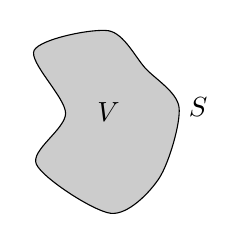
\begin{tikzpicture}
	\draw[->,fill=lightGray] plot [smooth cycle, samples=8,domain={1:8}] (\x*360/8+5*rnd:0.5cm+1cm*rnd) node[right] {$S$};
	\node at (0,0) {$V$};
\end{tikzpicture}
\end{center}
The amount of probability flowing out of the surface is equal to the rate of change of the probability density. In relativistic notation, the \ul{4-current} is
\begin{equation}
j^{\mu}=(\rho,\vec{j})
\end{equation}
Thus, the continuity equation should look like $\pd{\mu}j^{\mu}=0$.\\

From the Klein-Gordon equation
\begin{equation}
\pdv[2]{\psi}{t}=\vec{\nabla}^{2}\psi-m^{2}\psi\qq{and}\pdv[2]{\psi^{*}}{t}=\vec{\nabla}^{2}\psi^{*}-m^{2}\psi^{*}
\end{equation}
Taking their difference with weights $\psi^{*}$ and $\psi$ respectively
\begin{equation}
\begin{aligned}
\psi^{*}\pdv[2]{\psi}{t}-\psi\pdv[2]{\psi^{*}}{t}&=\psi^{*}\vec{\nabla}^{2}\psi-\psi\vec{\nabla}^{2}\psi^{*}\\
\pdv{t}\qty(\psi^{*}\pdv{\psi}{t}-\psi\pdv{\psi^{*}}{t})&=\vec{\nabla}\cdot\qty(\psi^{*}\vec{\nabla}\psi-\psi\vec{\nabla}\psi^{*})
\end{aligned}
\end{equation}
If one defines $\vec{j}=-\frac{i}{2m}\qty(\psi^{*}\vec{\nabla}\psi-\psi\vec{\nabla}\psi^{*})$ and $\rho(\vec{x},t)=-\frac{i}{2m}\qty(\psi^{*}\pdv{\psi}{t}-\psi\pdv{\psi^{*}}{t})$, then one obtains
\begin{equation}
\begin{aligned}
-\pdv{\rho}{t}&=\vec{\nabla}\cdot\vec{j}\\
\pdv{\rho}{t}+\vec{\nabla}\cdot\vec{j}&=0\\
\pd{\mu}j^{\mu}&=0\qq{as expected}
\end{aligned}
\end{equation}
However, the plane-wave solution $\psi(x^{\mu})=Ne^{ip^{\mu}x_{\mu}}$ yields a $\rho(x^{\mu})$ that is not positive-definite. Thus, $\rho(x^{\mu})$ cannot have the meaning of a probability density. This is connected to the existence of the negative energy solution. Furthermore, the wavefunction $\psi$ in the Klein-Gordon equation is scalar and thus cannot describe an electron with spin.

\subsection{Dirac Equation}
Dirac realized that in order to describe a relativistic electron, one needs to find a Lorentz-invariant equation that is first order in time, similar to the Schr\"{o}dinger equation. If the equation is linear in time, it has the form
\begin{equation}
\qty(c^{\mu}\pd{\mu}-m)\psi=0
\end{equation}
However, if $c^{\mu}$ are simply four complex numbers, then $c^{\mu}$ implies a preferred direction in space-time, meaning the equation would not be Lorentz invariant. Thus, $c^{\mu}$ cannot simple be numbers. Let $c^{\mu}=i\gamma^{\mu}$.
\begin{equation}
\qty(i\gamma^{\mu}\pd{\mu}-m)\psi=0
\end{equation}
This equation must still give the energy eigenvalues $E=\pm\sqrt{\pm\vec{p}^{2}+m^{2}}$. Using the plane-wave leads to the same problem as before, so instead let us multiply on the left by $\qty(i\gamma^{\mu}\pd{\mu}+m)$.
\begin{equation}
\begin{aligned}
(i\gamma^{\mu}\pd{\mu}+m)(i\gamma^{\mu}\pd{\mu}-m)\psi&=0\\
(-\gamma^{\mu}\pd{\mu}\gamma^{\nu}\pd{\nu}-m^{2}-\cancel{mi\gamma^{\mu}\pd{\mu}}+\cancel{mi\gamma^{\nu}\pd{\nu}})\psi&=0\\
(\gamma^{\mu}\gamma^{\nu}\pd{\mu}\pd{\nu}+m^{2})\psi&=0
\end{aligned}
\end{equation}
These two terms cancel since both $\mu$ and $\nu$ are summed from 0 to 3. This will turn to the Klein-Gordon equation if
\begin{equation}
\gamma^{\mu}\gamma^{\nu}\pd{\mu}\pd{\nu}=\pd{\mu}\pu{\mu}=\eta^{\mu\nu}\pd{\mu}\pd{\nu}\qq{(i.e. if $\gamma^{\mu}\gamma^{\nu}=\eta^{\mu\nu}$)}
\end{equation}
where $\eta^{\mu\nu}$ is the \ul{Minkowski metric tensor} with
\begin{itemize}
\item $\eta^{00}=1$
\item $\eta^{11}=\eta^{22}=\eta^{33}=-1$
\item $\eta^{ij}=0$ if $i\neq j$
\item $\eta^{\mu\nu}\pd{\mu}\pd{\nu}=\pd[2]{t}-\pd[2]{x}-\pd[2]{y}-\pd[2]{z}$
\item $a^{\mu}=\eta^{\mu\nu}a_{\nu}$
\end{itemize}
Since $\eta^{\mu\nu}=\eta^{\nu\mu}$ is symmetric, one can write $\eta^{\mu\nu}$ as
\begin{equation}
\eta^{\mu\nu}=\frac{1}{2}(\eta^{\nu\mu}+\eta^{\mu\nu})=\frac{1}{2}(\gamma^{\mu}\gamma^{\nu}+\gamma^{\nu}\gamma^{\mu})=\frac{1}{2}\acomm{\gamma^{\mu}}{\gamma^{\nu}}
\end{equation}
This condition defines \ul{Clifford algebra}. THus
\begin{itemize}
\item $(\gamma^{0})=1$
\item $(\gamma^{1})^{2}=(\gamma^{2})^{2}=(\gamma^{3})^{2}=-1$
\item $\gamma^{\mu}\gamma^{\nu}=-\gamma^{\nu}\gamma^{\mu}$ since $\gamma^{\mu}$ and $\gamma^{\nu}$ anti-commute when $\mu\neq\nu$
\end{itemize}
This implies $\gamma^{\mu}$ cannot be ordinary numbers.\\

One can write the Dirac equation now as
\begin{equation}
(\underbrace{i\gamma^{0}\pd{t}}_{\trm{time}}+\underbrace{i\gamma^{i}\pd{i}}_{\trm{space}}-m)\psi=0,\quad i\in\{1,2,3\}
\end{equation}
Multiplying by $\gamma^{0}$ on the left
\begin{equation}
\begin{aligned}
(i\pd{t}+i\gamma^{0}\gamma^{i}\pd{i}-m\gamma^{0})\psi&=0\\
i\pd{t}\psi&=(-i\gamma^{0}\gamma^{i}\pd{i}+m\gamma^{0})\psi
\end{aligned}
\end{equation}
This defines the \ul{Dirac Hamiltonian} as
\begin{equation}
\begin{aligned}
\vb{H}&=-i\gamma^{0}\gamma^{i}\pd{i}+m\gamma^{0}\\
&\quad\explain{Since $i\pdv{\psi}{t}\psi=\vb{H}\psi$}
\end{aligned}
\end{equation}
Note that $\gamma^{\mu}\pd{\mu}=\gamma^{0}\pd{t}+\gamma^{1}\pd{x}+\gamma^{2}\pd{y}+\gamma^{3}\pd{z}$ is an Einstein sum.\\

What is the nature of $\gamma^{\mu}$? Since $\gamma^{\mu}$ are not ordinary numbers, one suspects they must be matrices. They cannot be $2\times2$ matrices, since these can always be expanded as a linear combination of the unit matrix and Pauli spin matrices, which do not satisfy Clifford algebra. It turns out $\gamma^{\mu}$ must be $4\times4$ \ul{gamma matrices}. $\gamma^{\mu}$ forms a basis for $4\times4$ Hermitian matrices. Their representation is
\begin{equation}
\begin{aligned}
\gamma^{0}&=\mqty[\mathbb{I} & 0 \\ 0 & -\mathbb{I}]=\mathbb{I}\otimes\Tau_{3}\equiv\mathbb{I}\Tau_{3},\quad&\Tau_{3}=\mqty[1 & 0 \\ 0 & -1]\\
\gamma^{i}&=\mqty[0 & \sigma^{i} \\ -\sigma^{i} & 0]=i\sigma^{i}\otimes\Tau_{2}\equiv i\sigma^{i}\Tau_{2},\quad&\Tau_{2}=\mqty[0 & -i \\ i & 0]
\end{aligned}
\end{equation}
Note both $\sigma^{i}$ and $\Tau_{i}$ are the standard $2\times2$ Pauli spin matrices. Clifford algebra when $(\sigma^{i})^{2}=(\Tau_{i})^{2}=\mathbb{I}$ and $\sigma^{i}\sigma^{j}=-\sigma^{j}\sigma^{i}$ when $i\neq j$. One can see now that
\begin{equation}
\begin{aligned}
(\gamma^{0})^{2}&=(\mathbb{I}\otimes\Tau_{3})^{2}=\mathbb{I}^{2}\otimes\Tau_{3}^{2}=\mathbb{I}\otimes\mathbb{I}=\mathbb{I}\\
(\gamma^{i})^{2}&=(i\sigma^{i}\otimes\Tau_{2})^{2})^{2}=-\mathbb{I}\otimes\mathbb{I}=-\mathbb{I}\\
\gamma^{i}\gamma^{j}&=(i\sigma^{i}\otimes\Tau_{2})(i\sigma^{j}\otimes\Tau_{2}),\quad i\neq j\\
&=-\sigma^{i}\sigma^{j}\otimes\id\\
&=\sigma^{j}\sigma^{i}\otimes\id\\
&=-(i\sigma^{j}\otimes\Tau_{2})(i\sigma^{i}\otimes\Tau_{2})\\
&=-\gamma^{j}\gamma^{i}
\end{aligned}
\end{equation}
Define $\alpha_{i}=\gamma^{0}\gamma^{i}$ and $\beta=\gamma^{0}$. The Dirac Hamiltonian then becomes
\begin{equation}
\begin{aligned}
\vb{H}&=-\vec{\alpha}\cdot\vec{\vb{p}}+\beta m,\quad\vb{p}_{i}=-i\pd{i}\\
&=-i\vec{\alpha}\cdot\vec{\nabla}+\beta m
\end{aligned}
\end{equation}
$\psi$ must then be a 4-component vector (spinor). $\psi^{\dagger}$ is now defined to be the complex conjugated row vector corresponding to the column vector $\psi$. The probability density
\begin{equation}
\rho=\psi^{\dagger}\psi=\abs{\psi_{1}}^{2}+\abs{\psi_{2}}^{2}+\abs{\psi_{3}}^{2}+\abs{\psi_{4}}^{2}
\end{equation}
is positive definite. Let us show $\rho$ satisfies a continuity equation.\\

Define $\vec{j}=\psi^{\dagger}\vec{\alpha}\psi$ as the probability current. From the Dirac equation
\begin{equation}
\begin{aligned}
i\pdv{\psi}{t}&=(-i\vec{\alpha}\cdot\vec{\nabla}+\beta m)\psi\\
-i\pdv{\psi^{\dagger}}{t}&=i\vec{\nabla}\psi^{\dagger}\cdot\vec{\alpha}+m\psi^{\dagger}\beta
\end{aligned}
\end{equation}
Note that both $\alpha_{i}$ and $\beta$ are Hermitian.\\

Taking the difference weighted by $\psi^{\dagger}$ and $\psi$ respectively.
\begin{equation}
\begin{aligned}
i\qty(\psi^{\dagger}\pdv{\psi}{t}+\pdv{\psi^{\dagger}}{t}\psi)&=-i\psi^{\dagger}\vec{\alpha}\cdot\vec{\nabla}\psi-i\vec{\nabla}\psi^{\dagger}\cdot\vec{\alpha}\psi\\
i\pdv{t}\qty(\psi^{\dagger}\psi)&=-i\vec{\nabla}\cdot(\psi^{\dagger}\vec{\alpha}\psi)\\
\pdv{\rho}{t}&=-\vec{\nabla}\cdot\vec{j}\\
\pdv{\rho}{t}+\vec{\nabla}\cdot\vec{j}&=0
\end{aligned}
\end{equation}
Thus, the Dirac equation immediately solves the issue of the lack of conserved probability density in the Klein-Gordon equation.\\

Introduce the \ul{Dirac adjoint} $\overline{\psi}=\psi^{\dagger}\gamma^{0}$ to simplify the notation.
\begin{equation}
\begin{aligned}
\rho&=\psi^{\dagger}\psi=\psi^{\dagger}\overbrace{\gamma^{0}\gamma^{0}}^{\id}\psi=\overline{\psi}\gamma^{0}\psi\\
\vec{j}&=\psi^{\dagger}\vec{\alpha}\psi=\psi^{\dagger}\gamma^{0}\vec{\gamma}\psi=\overline{\psi}\vec{\gamma}\psi\qq{where $\vec{\gamma}=(\gamma^{1},\gamma^{2},\gamma^{3})$}
\end{aligned}
\end{equation}
Thus, the continuity equation in covariant form is
\begin{equation}
\pdv{t}(\overline{\psi}\gamma^{0}\psi)+\vec{\nabla}\cdot(\overline{\psi}\vec{\gamma}\psi)=\pd{\mu}j^{\mu}=0
\end{equation}
where $j^{\mu}=\overline{\psi}\gamma^{\mu}\psi=(\rho,\vec{j})$ is the \ul{4-current vector}.\\

Solve the Dirac equation by looking for plane-wave solutions $\psi=Ne^{i(\vec{p}\cdot\vec{x}-Et)}$. Plugging into the Dirac equation
\begin{equation}
E\psi=(\vec{\alpha}\cdot\vec{p}+\beta m)\psi
\end{equation}
This is an eigenvalue problem for a $4\times4$ matrix.
\begin{equation}
\begin{aligned}
\gamma^{0}&=\id\otimes\Tau_{3}\equiv\Tau_{3}\\
\gamma^{i}&=i\sigma^{i}\otimes\Tau_{2}\equiv i\sigma^{i}\Tau_{2}\\
\implies\vb{H}(\vec{p})&=\vec{\alpha}\cdot\vec{p}+\beta m\\
&=\alpha_{i}p_{i}+\beta m\\
&=\gamma^{0}\gamma^{i}p_{i}+\beta m\\
&=\Tau_{3}(i\sigma^{i}\Tau_{2})p_{i}+\Tau_{3}m\\
&=i\sigma^{i}\Tau_{3}\Tau_{2}p_{i}+m\Tau_{3}\\
&\quad\explain{Since $\sigma^{i}$ and $\Tau_{i}$ act on different Hilbert spaces, they commute. Note however the $\Tau_{i}$ do not commute when each other.}\\
&=i\sigma^{i}(-i\Tau_{1})p_{i}+m\Tau_{3}\\
&=\Tau_{1}\vec{\sigma}\cdot\vec{p}+m\Tau_{3}\\
&=(\vec{\sigma}\cdot\vec{p})\otimes\Tau_{1}+m\id\otimes\Tau_{3}\\
\implies\vb{H}&=\mqty[m & \vec{\sigma}\cdot\vec{p} \\ \vec{\sigma}\cdot\vec{p} & -m]
\end{aligned}
\end{equation}
One can diagonalize $\vec{\sigma}\cdot\vec{p}$ independently from the rest of $\vb{H}$, since $\vec{\sigma}\cdot\vec{p}$ acts on a different vector space than $\Tau_{i}$ and $m$ is a constant.
\begin{equation}
\begin{aligned}
\vec{\sigma}\cdot\vec{p}=\mqty[p_{z} & p_{x}-ip_{y} \\ p_{x}+ip_{y} & -p_{z}]
\end{aligned}
\end{equation}
The eigenvalues are
\begin{equation}
\begin{aligned}
0&=\det(\vec{\sigma}\cdot\vec{p}-\epsilon\id)\\
\implies \epsilon&=\pm\vec{p}=\pm\sqrt{p_{x}^{2}+p_{y}^{2}+p_{z}^{2}}
\end{aligned}
\end{equation}
$\epsilon=p$ corresponds to $\expval{\vec{\sigma}}$ lying along $\vec{p}$, whereas $\epsilon=-p$ corresponds to $\expval{\vec{\sigma}}$ lying opposite to $\vec{p}$. The projection of spin onto momentum is called \ul{helicity}. If $\expval{\vec{\sigma}\cdot\vec{p}}$ is positive ($\vec{\sigma}$ lies along $\vec{p}$), one has \ul{right-handed helicity}. Otherwise, if $\expval{\vec{\sigma}\cdot\vec{p}}$ is negative ($\vec{\sigma}$ lies opposite to $\vec{p}$), one has \ul{left-handed helicity}.\\

The diagonalization of $\vec{\sigma}\cdot\vec{p}$ means transforming the $4\times 4$ matrix $\vb{H}$ into block diagonal form.
\begin{equation}
\vb{H}=\mqty[\vb{H}_{R} & 0 \\ 0 & \vb{H}_{L}]
\end{equation}
where $\vb{H}_{R}=\Tau_{1}p+m\Tau_{3}$ and $\vb{H}_{L}=-\Tau_{1}p+m\Tau_{3}$.\\

The eigenvalues of both $\vb{H}_{R}$ and $\vb{H}_{L}$ are identical and equal to $E_{p}=\pm\sqrt{p^{2}+m^{2}}$. Each eigenstate is doubly degenerate, corresponding to each possible helicity. However, one still has the negative energy problem. A particle would want to ``fall to the bottom" to minimize its energy, but there is no bottom. Dirac proposed a solution based on Pauli's exclusion principle. Electrons are fermions and fermions were experimentally found to obey Pauli's exclusion principle. In this case, two fermions cannot occupy the same state. Dirac's proposal states that in what one calls a vacuum is a state in which all the negative energy states are filled by fermions, such that an extra fermion in the positive energy state cannot fall down to negative energy states.
\begin{center}
\begin{tikzpicture}
	\draw[<->] (-4,0) -- (4,0) node[right] {$p$};
	\draw[<->] (0,-4) -- (0,4) node[above] {$E$};
	\draw[<->,domain=-3.46:3.46,samples=200] plot (\x,{sqrt((\x)^2+2)}) node[right] {$E=\sqrt{p^{2}+m^{2}}$};
	\draw[<->,domain=-3.46:3.46,samples=200] plot (\x,{-sqrt((\x)^2+2)}) node[right] {$E=-\sqrt{p^{2}+m^{2}}$};
	\draw[<->] (0.1,1.314) node[below right] {$2m$} -- (0.1,-1.314);
	\fill (-0.5,2) circle (2pt) node[above] {e$^{-}$};
	\fill (-0.5,-2) circle (2pt) node[below,yshift=-0.2cm] {e$^{-}$};
	\draw[->,shorten >=1mm] (-0.5,-2) -- (-0.5,2);
	\draw[->,shorten >=1mm,decorate,decoration={snake}] (-2.75,-4) -- (-0.5,-2);
\end{tikzpicture}
\end{center}
The group of negative energy states filled with fermions is called a \ul{Dirac} \ul{negative energy sea} and is unobservable. However, the lack of an electron in one of the negative energy states is observable as a positron, which is the anti-particle of an electron with the same mass, but with opposite charge. A photon can excite an electron out of this sea, leaving a positive energy electron and negative energy positron. These electron-positron pairs can annihilate and emit photons. These positrons have been observed experimentally. This picture works only for fermions, which have half-integer spin. Bosons require an analysis by Feynman.

\subsection{Spin}
Let us prove that $\vec{\sigma}$ is the spin. The mechanical momentum for a particle with charge $-e$ in an electromagnetic field is related to the canonical momentum as
\begin{equation}
m\vec{v}=\vec{p}+\frac{e}{c}\vec{A}=-i\vec{\nabla}+\frac{e}{c}\vec{A}\qq{(by correspondance principle)}
\end{equation}
where $\vec{p}$ is the canonical momentum from the Hamiltonian formalism and $\vec{A}$ is the vector potential.\\

Thus, for a free particle, since kinetic energy is $\frac{m\abs*{\vec{v}}^{2}}{2m}$, the non-relativistic Hamiltonian becomes (in natural units)
\begin{equation}
\vb{H}=\frac{1}{2}\qty(-i\vec{\nabla}+e\vec{A})^{2}
\end{equation}
Applying the same substitution in the Dirac Hamiltonian
\begin{equation}
\begin{aligned}
\vb{H}&=\tau_{1}\vec{\sigma}\cdot\qty(-i\vec{\nabla}+e\vec{A})+m\tau_{3}=\mqty[m & \vec{\sigma}\cdot(\vec{p}+e\vec{A}) \\ \vec{\sigma}\cdot(\vec{p}+e\vec{A}) & -m]\\
\therefore\vb{H}\psi&=E\psi\implies\mqty[m & \vec{\sigma}\cdot(\vec{p}+e\vec{A}) \\ \vec{\sigma}\cdot(\vec{p}+e\vec{A}) & -m]\mqty[u \\ v] =E\mqty[u \\ v]
\end{aligned}
\end{equation}
where $u$ and $v$ are two-component spinors.\\

In the non-relativistic limit, $p\l m$ and $E\approx m$. From the lower equation
\begin{equation}
\begin{aligned}
\vec{\sigma}\cdot(\vec{p}+e\vec{A})u-mv&=Ev\approx mv\\
\therefore \vec{\sigma}\cdot(\vec{p}+e\vec{A})u&=2mv\\
\implies v&=\frac{1}{2m}\vec{\sigma}\cdot(\vec{p}+e\vec{A})u
\end{aligned}
\end{equation}
From the top equation
\begin{equation}
\begin{aligned}
mu+\vec{\sigma}\cdot(\vec{p}+e\vec{A})v&=Eu\\
\frac{1}{2m}\vec{\sigma}\cdot(\vec{p}+e\vec{A})\vec{\sigma}\cdot(\vec{p}+e\vec{A})u&=(E-m)u
\end{aligned}
\end{equation}
For any vectors $\vec{\alpha}$ and $\vec{\beta}$
\begin{equation}
\begin{aligned}
(\vec{\sigma}\cdot\vec{\alpha})(\vec{\sigma}\cdot\vec{\beta})&=\sigma^{i}\alpha_{i}\sigma^{j}\beta_{j}\\
&=\frac{1}{2}\qty(\acomm{\sigma^{i}}{\sigma^{j}}+\comm{\sigma^{i}}{\sigma^{j}})\alpha_{i}\beta_{j}\\
&=(\delta_{ij}+i\varepsilon_{ijk}\sigma^{k})\alpha_{i}\beta_{j}\\
&=\vec{\alpha}\cdot\vec{\beta}+i\vec{\sigma}\cdot(\vec{\alpha}\times\vec{\beta})
\end{aligned}
\end{equation}

Thus
\begin{equation}
(E-m)u=\frac{1}{2m}\qty(\vec{p}+e\vec{A})^{2}u+\frac{i}{2m}\vec{\sigma}\cdot\underbrace{\qty[(\vec{p}+e\vec{A})\times(\vec{p}+e\vec{A})]}_{\neq0 \trm{ since }\vec{p}=-i\vec{\nabla}}u
\end{equation}
where
\begin{equation}
\begin{aligned}
\qty(\vec{p}+e\vec{A})\times\qty(\vec{p}+e\vec{A})u&=\qty(-i\vec{\nabla}+e\vec{A})\times\qty(-i\vec{\nabla}+e\vec{A})u\\
&=\cancelto{0}{-\vec{\nabla}\times\qty(\vec{\nabla}u)}-ie\vec{\nabla}\times\qty(\vec{A}u)-ie\vec{A}\times\vec{\nabla}u+\cancelto{0}{e^{2}\vec{A}\times\vec{A}u}\\
&=-ie\qty[\vec{\nabla}\times\qty(\vec{A}u)+\vec{A}\times\qty(\vec{\nabla}u)]\\
&=-ie\bigg[\qty(\vec{\nabla}\times\vec{A})u+\cancelto{0}{\qty(\vec{\nabla}u)\times\vec{A}+\vec{A}\times\qty(\vec{\nabla}u)}\bigg]\\
&=-ie\vec{B}u
\end{aligned}
\end{equation}
Therefore
\begin{equation}
(E-m)u=\frac{1}{2m}\qty(\vec{p}+e\vec{A})^{2}u+\frac{e}{2m}\vec{\sigma}\cdot\vec{B}u
\end{equation}
Since $\vec{S}=\frac{1}{2}\vec{\sigma}$ (in natural units)
\begin{equation}
\qty(\frac{e}{2m}\vec{\sigma}\cdot\vec{B})=2\qty(\frac{e}{2m}\vec{S}\cdot\vec{B})
\end{equation}

\aside{Note that $2\qty(\frac{e}{2m}\vec{S}\cdot\vec{B})=g\mu_{B}\vec{S}\cdot\vec{B}=-\vec{\mu}\cdot\vec{B}$, where $g\approx 2$ is the gyroscopic ratio for electrons, $\mu_{B}=\frac{e\hbar}{2mc}$ is the Bohr magneton, and $\vec{\mu}=-g\mu_{B}\vec{S}$ is the magnetic dipole moment.}\\
Thus
\begin{equation}
\begin{aligned}
\underbrace{(E-m)}_{\trm{kinetic energy}}&u=\frac{1}{2m}\qty(\vec{p}+e\vec{A})^{2}u-\vec{\mu}\cdot\vec{B}u\\
\frac{1}{2m}\qty(-i\vec{\nabla}+e\vec{A})^{2}&u-\vec{\mu}\cdot\vec{B}u=\vb{T}u
\end{aligned}
\end{equation}
This is the non-relativistic Schr\"{o}dinger equation for an electron in a magnetic field. The existence of spin follows from combining quantum mechanics and special relativity. This combination also leads to anti-particles. If we had solved for $v$ instead, this would simply lead to the spinor of the anti-particle.\\

In the non-relativistic limit
\begin{equation}
E=\sqrt{m^{2}+p^{2}}=m\sqrt{1+\frac{p^{2}}{m^{2}}}\approx m\qty(1+\frac{p^{2}}{2m^{2}})=m+\frac{p^{2}}{2m}
\end{equation}
Thus, one can see the Dirac equation predicts the contribution of $-\vec{\mu}\cdot\vec{B}$ due to the spin of the particle.

\subsection{Ultrarelativistic limit}
In the ultrarelativistic limit, $p\gg m$ and $E\approx p$, a characteristic called chirality occurs. Let us introduce a new matrix called $\gamma^{5}$ (named as such due to historical reasons).
\begin{equation}
\gamma^{5}=i\gamma^{0}\gamma^{1}\gamma^{2}\gamma^{3}
\end{equation}
In Dirac representation, $\gamma^{0}=\tau_{3}$ and $\gamma^{i}=i\sigma^{i}\tau_{2}$.
\begin{equation}
\begin{aligned}
\therefore\gamma^{5}&=i\qty(\tau_{3})\qty(i\sigma^{1}\tau_{2})\qty(i\sigma^{2}\tau_{2})\qty(i\sigma^{3}\tau_{2})\\
&=\sigma^{1}\sigma^{2}\sigma^{3}\tau_{3}\tau_{2}^{3}\\
&=\sigma^{1}\sigma^{2}\sigma^{3}\tau_{3}\tau_{2}\\
&\quad\explain{Since $\tau_{2}^{2}=\mathbb{I}$}
\end{aligned}
\end{equation}
Note that
\begin{equation}
\begin{aligned}
\tau_{3}\tau_{2}&=\mqty[1 & 0 \\ 0 & -i]\mqty[0 & -i \\ i & 0]=\mqty[0 & -i \\ -i & 0]=-i\tau_{1}\\
\sigma^{1}\sigma^{2}&=\mqty[0 & 1 \\ 1 & 0]\mqty[0 & -i \\ i & 0]=\mqty[i & 0\\ 0 & -i]=i\sigma^{3}
\end{aligned}
\end{equation}
Therefore
\begin{equation}
\begin{aligned}
\gamma^{5}&=i\qty(\sigma^{3})^{2}\qty(-i\tau_{1})\\
&=\tau_{1}
\end{aligned}
\end{equation}
The Dirac Hamiltonian is
\begin{equation}
\qty(\tau_{1}\vec{\sigma}\cdot\vec{p}+m\tau_{3})\psi=E\psi
\end{equation}
In the non-relativistic limit, $p\ll m$. Thus
\begin{equation}
\begin{aligned}
m\tau_{3}\psi&=E\psi \qq{($p$ treated as though $p=0$)}\\
m\mqty[\mathbb{I} & 0 \\ 0 & -\mathbb{I}]\psi&=E\psi\\
\implies E&=\pm m
\end{aligned}
\end{equation}
In Dirac representation, the Dirac Hamiltonian becomes diagonal in the non-relativistic limit. This is no true in the ultrarelativistic limit. Note $\gamma^{0}$ is diagonal in this representation.\\

In Weyl representation, let $\gamma^{0}=\tau_{1}$ and $\gamma^{i}=i\sigma^{i}\tau_{2}$. Thus
\begin{equation}
\begin{aligned}
\gamma^{5}&=i\gamma^{0}\gamma^{1}\gamma^{2}\gamma^{3}\\
&=i(\tau_{1})(i\sigma^{1}\tau_{2})(i\sigma^{2}\tau_{2})(i\sigma^{3}\tau_{2})\\
&=(\sigma^{1}\sigma^{2}\sigma^{3})(\tau_{1}\tau_{2}^{3})\\
&=i(\tau_{1}\tau_{2})\\
&=i(i\tau_{3})\\
&=-\tau_{3}
\end{aligned}
\end{equation}
In this representation, the Dirac Hamiltonian becomes
\begin{equation}
\begin{aligned}
\vb{H}&=\vec{\alpha}\cdot\vec{p}+\beta m\\
&=\alpha_{i}p_{i}+\beta m\\
&=\gamma^{0}\gamma^{i}p_{i}+\gamma^{0}m\\
&=\tau_{1}(i\sigma^{i}\tau_{2})p_{o}+\tau_{1}m\\
&=i\sigma^{i}(i\tau_{3})p_{i}+m\tau_{1}\\
&=-\tau_{3}\sigma^{i}p_{i}+m\tau_{1}\\
&=-\tau_{3}\vec{\sigma}\cdot\vec{p}+m\tau_{1}\\
&=\mqty[-\vec{\sigma}\cdot\vec{p} & m \\ m & \vec{\sigma}\cdot\vec{p}]
\end{aligned}
\end{equation}
In the limit $m=0$ (i.e. massless particles), the upper and lower blocks of $\vb{H}$ decouple and the matrix becomes block diagonal. One gets two independent $2\times 2$ equations instead of a single $4\times 4$ equation. This is the \ul{Weyl equation}. Two 2-component fermions are ``hiding" in the 4-component Dirac fermion.\\

One cannow write the Hamiltonian as two separate $2\times2$ Hamiltonians $\vb{H}=\pm \vec{\sigma}\cdot\vec{p}$. Let $\vb{H}_{L}=-\vec{\sigma}\cdot\vec{p}$ and $\vb{H}_{R}=\vec{\sigma}\cdot\vec{p}$. Thus the Weyl equations are
\begin{equation}
\begin{aligned}
i\pdv{\psi_{L}}{t}&=\vb{H}_{L}\psi_{L}\\
i\pdv{\psi_{R}}{t}&=\vb{H}_{R}\psi_{R}
\end{aligned}
\end{equation} 
where $\psi_{L}$ describes the particle with left-handed chirality while $\psi_{R}$ describes the particle with right-handed chirality.\\

\aside{Chirality is an eigenvale of $\gamma^{5}$ equal to $\pm1$.}\\

Solving for $\psi_{L}$
\begin{equation}
i\pdv{\psi_{L}}{t}=\vb{H}_{L}\psi_{L}=-\vec{\sigma}\cdot\vec{p}\psi_{L}=i\vec{\sigma}\cdot\vec{\nabla}\psi_{L}
\end{equation}
\begin{equation}
i\pdv{\psi_{R}}{t}=\vb{H}_{R}\psi_{R}=\vec{\sigma}\cdot\vec{p}\psi_{R}=-i\vec{\sigma}\cdot\vec{\nabla}\psi_{R}
\end{equation}
We introduce the notation
\begin{equation}
\sigma^{\mu}=(\mathbb{I},\vec{\sigma})\quad\trm{and}\quad\overline{\sigma}^{\mu}=(\mathbb{I},-\vec{\sigma})
\end{equation}
Thus, the Weyl equations become
\begin{equation}
\begin{aligned}
\sigma^{\mu}\partial_{\mu}\psi_{R}&=0\\
\overline{\sigma}^{\mu}\partial_{\mu}\psi_{L}&=0
\end{aligned}
\end{equation}
Note that the $L$ and $R$ indices refer to left- or right-handed chirality. Massless fermions have another conserved quantum number called \ul{chirality}. Finite mass mixes the two chiralities.
\begin{equation}
\begin{aligned}
\gamma^{5}&=\mqty[-\mathbb{I} & 0 \\ 0 & \mathbb{I}]\\
\implies \gamma^{5}\psi_{L}&=-\psi_{L}\\
\gamma^{5}\psi_{R}&=\psi_{R}\qq{since $\vb{H}=\vec{\sigma}\cdot\vec{p}\gamma^{5}$}
\end{aligned}
\end{equation}
Thus, one can see that $\gamma^{5}$ is the chirality operator.\\

Weyl fermions (massless chiral fermions) are the elementary building blocks of matter.\\

Another useful way to see the conservation of chirality is to derive the continuity equation for chirality current. For our ordinary 4-current $j^{\mu}=(\rho,\vec{j})=(\psi^{\dagger}\psi,\psi^{\dagger}\vec{\alpha}\psi)$. One can conveniently rewrite this in terms of the Dirac adjoint such that
\begin{equation}
j^{\mu}=\overline{\psi}\gamma^{\mu}\psi
\end{equation}
where $\overline{\psi}=\psi^{\dagger}\gamma^{0}$ is the Dirac adjoint. Thus, the continuity equations becomes
\begin{equation}
\partial_{\mu}j^{\mu}=0
\end{equation}
In this example, this expresses the conservation of particle number (charge conservation).\\

Let us define the \ul{chiral 4-current}.
\begin{equation}
\begin{aligned}
j_{5}^{\mu}&=\overline{\psi}\gamma^{\mu}\gamma^{5}\psi\\
\therefore j_{5}^{0}&=\psi^{\dagger}\gamma^{5}\psi=\psi_{R}^{\dagger}\psi_{R}-\psi_{L}^{\dagger}\psi_{L}\\
\vec{j}_{5}&=\psi^{\dagger}\vec{\alpha}\gamma^{5}\psi=\psi_{R}^{\dagger}\vec{\alpha}\psi_{R}-\psi_{L}^{\dagger}\vec{\alpha}\psi_{L}
\end{aligned}
\end{equation}
Note that chiral charge is the difference between the right-handed charge and left-handed charge.
\begin{equation}
\begin{aligned}
\partial_{\mu}j_{5}^{\mu}&=\partial_{\mu}(\overline{\psi}\gamma^{\mu}\gamma^{5}\psi)\\
&=(\partial_{\mu}\overline{\psi})\gamma^{\mu}\gamma^{5}\psi+\overline{\psi}\gamma^{\mu}\gamma^{5}(\partial_{\mu}\psi)
\end{aligned}
\end{equation}
From the Dirac equation
\begin{equation}
 (i\gamma^{\mu}\partial_{\mu}-m)\psi=0
\end{equation}
Since $\gamma^{5}$ anti-commutes with all $\gamma^{\mu}$
\begin{equation}
\begin{aligned}
\gamma^{\mu}\gamma^{5}\partial_{\mu}\psi&=-\gamma^{5}\gamma^{\mu}\partial_{\mu}\psi=im\gamma^{5}\psi\qq{from Dirac equation}\\
\implies \overline{\psi}\gamma^{\mu}\gamma^{5}\partial_{\mu}\psi&=im\overline{\psi}\gamma^{5}\psi
\end{aligned}
\end{equation}

From the Hermitian conjugate of the Dirac equation
\begin{equation}
\qty[\qty(i\gamma^{\mu}\partial_{\mu}-m)\psi]^{\dagger}=-i\partial_{\mu}\phi^{\dagger}\qty(\gamma^{\mu})^{\dagger}-m\psi^{\dagger}=0
\end{equation}
Since $\gamma^{0}=\tau_{1}$, $(\gamma^{0})^{\dagger}=\gamma^{0}$ is Hermitian. Similarly, since $\gamma^{i}=i\sigma^{i}\tau_{2}$, $(\gamma^{i})^{\dagger}=-\gamma^{i}$ is anti-Hermitian. Since $\tau_{1}\tau_{1}\tau_{1}=\tau_{1}$ and $\tau_{1}\tau_{2}\tau_{1}=-\tau_{2}$
\begin{equation}
(\gamma^{\mu})^{\dagger}=\gamma^{0}\gamma^{\mu}\gamma^{0}
\end{equation}
Thus, the Hermitian conjugate of the Dirac equation becomes
\begin{equation}
\begin{aligned}
-i\partial_{\mu}\psi^{\dagger}\gamma^{0}\gamma^{\mu}\gamma^{0}-m\psi^{\dagger}&=0\\
\implies \partial_{\mu}\overline{\psi}\gamma^{\mu}&=im\overline{\psi}\qq{(after multiplying $\gamma^{0}$ on the right)}\\
\implies(\partial_{\mu}\overline{\psi})\gamma^{\mu}\gamma^{5}\psi&=im\overline{\psi}\gamma^{5}\psi
\end{aligned}
\end{equation}
Thus
\begin{equation}
\partial_{\mu}j_{5}^{\mu}=im\overline{\psi}\gamma^{5}\psi+im\overline{\psi}\gamma^{5}\psi=2im\overline{\psi}\gamma^{5}\psi
\end{equation}
This is the \ul{chiral continuity equation}.

\aside{Illustrating a conserved quantity will create a continuity equation with the right hand side equal to zero.}\\

When $m=0$, one can see that $\partial_{\mu}j_{5}^{\mu}=0$. Thus, chiral charge is conserved for massless fermions. Note that in actuality, a more careful derivation of relativistic quantum mechanics leads to
\begin{equation}
\partial_{\mu}j_{5}^{\mu}=2im\overline{\psi}\gamma^{5}\psi+\underbrace{\frac{e^{2}}{16\pi^{2}}\varepsilon^{\mu\nu\alpha\beta}F_{\mu\nu}F_{\alpha\beta}}_{\trm{chiral anomaly}}
\end{equation}

\subsection{Symmetries of Dirac Equation}
\subsubsection{Parity}
We shall now consider the symmetries inherent in the Dirac equation of the free particle
\begin{equation}
i\pdv{t}\psi(\vec{x},t)=\vb{H}\psi(\vec{x},t)=E\psi(\vec{x},t)
\end{equation}
where
\begin{equation}
\vb{H}=-i\gamma^{0}\gamma^{i}\partial_{i}+m\gamma^{0}
\end{equation}
Under parity
\begin{equation}
x^{\mu}=(x^{0},\vec{x})=(t,\vec{x})\rightarrow(t,-\vec{x})=x^{\prime\mu}
\end{equation}
Multiplying $\gamma^{0}$ to the left of the Dirac equation
\begin{equation}
\begin{aligned}
\gamma^{0}\qty(i\gamma^{\mu}\partial_{\mu}-m)\psi&=\gamma^{0}(i\gamma^{0}\partial_{0}+i\gamma^{i}\partial_{i}-m)\psi\\
&=(i\gamma^{0}\partial_{0}-i\gamma^{i}\partial_{i}-m)\gamma^{0}\psi\\
&=(i\gamma^{\mu}\partial_{\mu}^{\prime}-m)\gamma^{0}\psi
\end{aligned}
\end{equation}
Note that
\begin{equation}
\begin{aligned}
\partial_{i}&=\pdv{x^{i}}\\
\implies-\partial_{i}&=-\pdv{x^{i}}\\
\implies-\partial_{\mu}&=\partial_{\mu}^{\prime}=\pdv{x^{\prime\mu}}
\end{aligned}
\end{equation}

Thus
\begin{equation}
\gamma^{0}(i\gamma^{\mu}\partial_{\mu}-m)\psi=(i\gamma^{\mu}\partial_{\mu}^{\prime}-m)\psi=0
\end{equation}
Thus, $\gamma^{0}\psi$ obeys the Dirac equation where $\partial_{\mu}^{\prime}$ are the derivatives in the inverted coordinates. This indicates that $\psi^{\prime}(x^{\prime\mu})=\gamma^{0}\psi(x^{\mu})$ is the solution of the Dirac equation under parity and that $\gamma^{0}$ is the parity operator.\\

From this, one can see the Dirac operator is parity invariant
\begin{equation}
\begin{aligned}
(\gamma^{0})^{\dagger}(i\gamma^{\mu}\partial_{\mu}-m)\gamma^{0}&=\gamma^{0}(i\gamma^{\mu}\partial{\mu}-m)\gamma^{0}\\
&=(i\gamma^{\mu}\partial_{\mu}^{\prime}-m)\gamma^{0}\gamma^{0}\\
&=(i\gamma^{\mu}\partial_{\mu}^{\prime}-m)
\end{aligned}
\end{equation}

Moreover, the gamma matrices under parity are
\begin{equation}
\begin{aligned}
(\gamma^{0})^{\dagger}\gamma^{0}\gamma^{0}&=(\gamma^{0})^{\dagger}=\gamma^{0}\\
(\gamma^{0})^{\dagger}\gamma^{i}\gamma^{0}&=-\gamma^{0}\gamma^{0}\gamma^{i}=-\gamma^{i}\\
(\gamma^{0})^{\dagger}\gamma^{5}\gamma^{0}&=\gamma^{0}(i\gamma^{0}\gamma^{1}\gamma^{2}\gamma^{3})\gamma^{0}\\
&=-\gamma^{0}(i\gamma^{0}\gamma^{1}\gamma^{2})\gamma^{0}\gamma^{3}\\
&=\gamma^{0}(i\gamma^{0}\gamma^{1})\gamma^{0}(\gamma^{2}\gamma^{3})\\
&=-\gamma^{0}(i\gamma^{0}\gamma^{0})(\gamma^{1}\gamma^{2}\gamma^{3})\\
&=-i\gamma^{0}\gamma^{1}\gamma^{2}\gamma^{3}\\
&=-\gamma^{4}
\end{aligned}
\end{equation}
Thus, $\gamma^{0}$ is even under parity and $\gamma^{i}$ and $\gamma^{5}$ are odd under parity. This makes sense as $\gamma^{5}$ is the chirality operator.
\begin{center}
\begin{tikzpicture}
	\draw[->] (0,0,0) -- (2,0,0) node[right] {$\hat{y}$};
	\draw[->] (0,0,0) -- (0,2,0) node[above] {$\hat{z}$};
	\draw[->] (0,0,0) -- (0,0,2) node[below left] {$\hat{x}$};
	\draw[->] (3,1,0) -- (5,1,0);
	\draw[->] (8,1,0) -- (6,1,0) node[left] {$\hat{y}$};
	\draw[->] (8,1,0) -- (8,-0.5,0) node[below] {$\hat{z}$};
	\draw[->] (8,1,0) -- (8,1,-2) node[above right] {$\hat{x}$};
\end{tikzpicture}
\end{center}
One will show later that $\gamma^{5}$ is even under time-reversal, which will also imply $\gamma^{5}$ is the chirality operator.

\subsubsection{Charge Conjugation}
In the presence of an electromagnetic field, the Dirac equation becomes
\begin{equation}
[i\gamma^{\mu}(\partial_{\mu}+ieA_{\mu})-m]\psi=0
\end{equation}
where $A^{\mu}=(A^{0},\vec{A})$. Taking the complex conjugate
\begin{equation}
[-i(\gamma^{\mu})^{*}(\partial_{\mu}-ieA_{\mu})-m]\psi^{*}=0\qq{(since $A^{\mu}$ is real)}
\end{equation}
In Dirac representation
\begin{equation}
\begin{aligned}
\gamma^{0}&=\tau_{3} \quad\trm{and} &\gamma^{i}&=i\sigma^{i}\tau_{2}\\
\implies(\gamma^{0})^{*}&=\tau_{3} \quad\trm{and} &(\gamma^{i})^{*}&=-i(\sigma^{i})^{*}\tau_{2}^{*}
\end{aligned}
\end{equation}
Moreover
\begin{equation}
\begin{aligned}
(\gamma^{1})^{*}&=\gamma^{1}\\
(\gamma^{2})^{*}&=-\gamma^{2}\\
(\gamma^{3})^{*}&=\gamma^{3}
\end{aligned}
\end{equation}
The gamma matrices are defined by satisfying Clifford algebra. One property required is that
\begin{equation}
\frac{1}{2}\acomm{\gamma^{\mu}}{\gamma^{\nu}}=\eta^{\mu\nu}
\end{equation}
One sees that
\begin{equation}
\frac{1}{2}\acomm{-(\gamma^{\mu})^{*}}{-(\gamma^{\nu})^{*}}=\eta^{\mu\nu}
\end{equation}
Thus, $-(\gamma^{\mu})^{*}$ also satisfies Clifford algebra and are also a legitimate gamma matrix representation in the same basis. There exists a transformation $\mathcal{C}$ such that
\begin{equation}
-(\gamma^{\mu})^{*}=\mathcal{C}^{\dagger}\gamma^{\mu}\mathcal{C}
\end{equation}

Substituting in the Dirac equation
\begin{equation}
\begin{aligned}
[i\mathcal{C}^{\dagger}\gamma^{\mu}\mathcal{C}(\partial_{\mu}-ieA_{\mu})-m]\psi^{\dagger}&=0\\
\mathcal{C}^{\dagger}[i\gamma^{\mu}\mathcal{C}(\partial_{\mu}-ieA_{\mu})-m\mathcal{C}]\psi^{\dagger}&=0\\
\mathcal{C}^{\dagger}[i\gamma^{\mu}(\partial_{\mu}-ieA_{\mu})-m]\mathcal{C}\psi^{\dagger}&=0\\
[i\gamma^{\mu}(\partial_{\mu}-ieA_{\mu})-m]\mathcal{C}\psi^{\dagger}&=0\\
[i\gamma^{\mu}(\partial_{\mu}-ieA_{\mu})-m]\psi_{\mathcal{C}}&=0\\
\end{aligned}
\end{equation}
where $\gamma_{\mathcal{C}}=\mathcal{C}\psi^{*}$. This is the charge-conjugation Dirac equation. Moreover, it is the Dirac equation for the positron.\\

Let us find the matrix $\mathcal{C}$.
\begin{equation}
\begin{aligned}
-(\gamma^{\mu})^{*}&=\mathcal{C}^{\dagger}\gamma^{\mu}\mathcal{C}\\
\implies \mathcal{C}(\gamma^{\mu})^{*}&=-\gamma^{\mu}\mathcal{C}
\end{aligned}
\end{equation}
Thus, $\mathcal{C}$ commutes with $\gamma^{2}$ and anti-commutes with $\gamma^{0}$, $\gamma^{1}$, and $\gamma^{3}$. Therefore, $\mathcal{C}=\gamma^{2}$, with $\gamma^{2}$ being the charge-conjugation operator.
\begin{equation}
\psi_{\mathcal{C}}=\gamma^{2}\psi^{*}
\end{equation}

\subsubsection{Time-Reversal}
The Dirac equation is
\begin{equation}
i\pdv{\psi}{t}=\vb{H}\psi
\end{equation}
where 
\begin{equation}
\vb{H}=-i\gamma^{0}\gamma^{i}\partial_{i}+\gamma^{0}m
\end{equation}
Under time-reversal, one wants the Dirac equation to be of the form
\begin{equation}
i\pdv{t^{\prime}}\psi^{\prime}(t^{\prime})=\vb{H}\psi^{\prime}(t^{\prime})
\end{equation}
where $t^{\prime}=-t$ and $\psi^{\prime}(t^{\prime})=\Theta\psi(t)$.\\

We know that $\Theta=UK$. We need that $\Theta\vb{H}\Theta^{-1}=\vb{H}$. It is more convenient to write this condition as $\Theta^{-1}\vb{H}\Theta=\vb{H}$.
\begin{equation}
\therefore KU^{\dagger}\gamma^{0}UK=\gamma^{0} \quad\trm{and}\quad KU^{\dagger}(i\gamma^{0}\gamma^{i})UK=i\gamma^{0}\gamma^{i}
\end{equation}
This is so that $\vb{H}$ is even under parity.\\

Multiplying on the left and right by $K$
\begin{equation}
U^{\dagger}\gamma^{0}U=\gamma^{0}\qq{since $\gamma^{0}$ is real (in the Dirac and Weyl basis)}
\end{equation}
Similarly for $i\gamma^{0}\gamma^{i}$
\begin{equation}
\begin{aligned}
U^{\dagger}(i\gamma^{0}\gamma^{i})U&=K(i\gamma^{0}\gamma^{i})K=-i\gamma^{0}(\gamma^{i})^{*}\\
\implies -i\gamma^{0}(\gamma^{i})^{*}&=U^{\dagger}(i\gamma^{0})UU^{\dagger}\gamma^{i}U\\
&=i\gamma^{0}U^{\dagger}\gamma^{i}U\qq{since $U^{\dagger}\gamma^{0}U=\gamma^{0}$}\\
\implies U^{\dagger}\gamma^{i}U&=-(\gamma^{i})^{*}
\end{aligned}
\end{equation}
Since only $\gamma^{2}$ involves $i$ in the Dirac and Weyl basis, $U$ commutes with $\gamma^{2}$. Thus, $U$ commutes with $\gamma^{0}$ and $\gamma^{2}$, but anti-commutes with $\gamma^{1}$ and $\gamma^{3}$.
\begin{equation}
\implies U=\gamma^{1}\gamma^{3}
\end{equation}
Since $\gamma^{1}=i\tau_{2}\sigma^{1}$ and $\gamma^{3}=i\tau_{2}\sigma^{3}$
\begin{equation}
\begin{aligned}
U&=(i\tau_{2}\sigma^{1})(i\tau_{2}\sigma^{3})\\
&=-(\tau_{2})^{2}\sigma^{1}\sigma^{3}\\
&=-\sigma^{1}\sigma^{3}\\
&=-\mqty[0 & 1 \\ 1 & 0]\mqty[1 & 0 \\ 0 & -1]\\
&=-\mqty[0 & -1 \\ 1 & 0]\\
&=\mqty[0 & 1 \\ -1 & 0]\\
&=i\sigma^{2}
\end{aligned}
\end{equation}
Thus, one obtains $U=i\sigma^{2}$, which is in agreement with results obtained earlier for the time-reversal operator acting on a spin-$\frac{1}{2}$ system. The difference in sign is simply a phase factor.\\

Under time-reversal
\begin{equation}
\begin{aligned}
\Theta\gamma^{5}\Theta^{-1}&=UK\gamma^{5}KU^{\dagger}\\
&=\gamma^{1}\gamma^{3}K(i\gamma^{0}\gamma^{1}\gamma^{2}\gamma^{3})K\gamma^{3}\gamma^{1}\\
&=\gamma^{1}\gamma^{3}(i\gamma^{0}\gamma^{1}\gamma^{2}\gamma^{3})\gamma^{3}\gamma^{1}\\
&=\gamma^{1}\gamma^{3}(\gamma^{3}\gamma^{1})(i\gamma^{0}\gamma^{1}\gamma^{2}\gamma^{3})\\
&=i\gamma^{0}\gamma^{1}\gamma^{2}\gamma^{3}\\
&=\gamma^{5}
\end{aligned}
\end{equation}
Thus, $\gamma^{5}$ is odd under parity and even under time-reversal. Thus, one can see that $\gamma^{5}$ is chirality.\\

We now have three fundamental symmetry operators in terms of gamma matrices.
\begin{equation}
\begin{aligned}
\gamma^{0}&\equiv\mathcal{P}\\
\gamma^{2}&\equiv\mathcal{C}\\
\gamma^{1}\gamma^{3}&\equiv\mathcal{T}\\
\therefore\mathcal{C}\mathcal{P}\mathcal{T}&=\gamma^{2}\gamma^{0}\gamma^{1}\gamma^{3}\propto\gamma^{5}
\end{aligned}
\end{equation}
The product of charge conjugation, parity, and time-reversal (CPT) is a very important symmetry. This is regarded to be the most fundamental symmetry in nature. No violations have been found.

\newpage
\section{Many Body Quantum Mechanics}
Most problems in nature involve many bodies. Even ``single particle" relativistic quantum mechanics is in fact a many particle problem due to the existence of the Dirac sea. Condensed matter and relativistic quantum mechanics are very similar in this aspect.\\

In classical mechanics, individual particle trajectories may be followed. Thus, particles may always be distinguished from each other. In quantum mechanics, this is impossible due to the uncertainty principle. Thus, identical particles are indistinguishable.

\subsection{Two Particle System}
Consider the problem of a two-particle system. Let $\ket{K^{\prime}}\ket{K^{\prime\prime}}$ be a state in which particle 1 has observables $K^{\prime}$ and particle 2 has observables $K^{\prime\prime}$. Note that $\ket{K^{\prime}}\ket{K^{\prime\prime}}$ is defined to be a direct product (or tensor product).\\

In principle, interchanging the systems produces a different state $\ket{K^{\prime\prime}}\ket{K^{\prime}}$ if $K^{\prime}\neq K^{\prime\prime}$. Moreover, $(\bra{K^{\prime}}\bra{K^{\prime\prime}})(\ket{K^{\prime\prime}}\ket{K^{\prime}})=\ip{K^{\prime}}{K^{\prime\prime}}\ip{K^{\prime\prime}}{K^{\prime}}=0$ if $K^{\prime}\neq K^{\prime\prime}$. Thus, they are orthogonal. However, in the case of quantum identical particles, the particles cannot be distinguished, due to the fact that the particles can not be traced.

\begin{center}
\begin{tikzpicture}
	\node[left] at (-4,-0.9993) {$2$}; 
	\node[left] at (-4,0.9993) {$1$};
	\draw[domain=-4:4,samples=200] plot (\x, {tanh(\x)}) node[right] {$2$};
	\draw[domain=-4:4,samples=200] plot (\x, {-tanh(\x)}) node[right] {$1$};
\end{tikzpicture}
\end{center}
Distinguishability lies on being able to specify a trajectory for the particles (i.e. specifying both $\vec{x}(t)$ and $\vec{p}(t)$). In quantum mechanics, $\vec{x}(t)$ and $\vec{p}(t)$ cannot be specified at the same time. Thus, the concept of trajectory does not exist and quantum particles are indistinguishable.\\

If one measures $K^{\prime}$ and $K^{\prime\prime}$ on the two particle system, due to the indistinguishability of the particles, one does not know which state that corresponds with our measurements. In principle, this can be any linear combination of $\ket{K^{\prime}}\ket{K^{\prime\prime}}$ and $\ket{K^{\prime\prime}}\ket{K^{\prime}}$
\[
c_{1}\ket{K^{\prime}}\ket{K^{\prime\prime}}+c_{2}\ket{K^{\prime\prime}}\ket{K^{\prime}}
\]
All kets of this form lead to an identical set of eigenvalues when a measurement is performed. This is known as \ul{exchange degeneracy}. This presents a difficulty as a specification of the eigenvalues of a complete set of observables does not completely determine the state ket.

\subsection{Permutation Operator}
Define the \ul{permutation operator} as
\begin{equation}
P_{12}\ket{K^{\prime}}\ket{K^{\prime\prime}}=\ket{K^{\prime\prime}}\ket{K^{\prime}}
\end{equation}
with
\begin{equation}
P_{12}=P_{21}
\end{equation}
and
\begin{equation}
P_{12}^{2}=\mathbb{I}
\end{equation}
Under $P_{12}$, particle 1 having $K^{\prime}$ becomes particle 1 having $K^{\prime\prime}$, while particle 2 having $K^{\prime\prime}$ becomes particle 2 having $K^{\prime}$. In other words, it as the effect of interchanging 1 and 2. Note that since $P_{12}^{2}=\mathbb{I}$, $P_{12}$ has eigenvalues $\pm1$.\\

Consider specifically the case where the two particle state is specified completely be eigenvalues of a Hermitian operator $\vb{A}$ for each of the particles.
\begin{align}
\vb{A}_{1}\ket{a^{\prime}}\ket{a^{\prime\prime}}&=a^{\prime}\ket{a^{\prime}}\ket{a^{\prime\prime}}\\
\vb{A}_{2}\ket{a^{\prime}}\ket{a^{\prime\prime}}&=a^{\prime\prime}\ket{a^{\prime}}\ket{a^{\prime\prime}}
\end{align}
where the subscripts on $\vb{A}$ denote the particle labels and $\vb{A}_{1}$ and $\vb{A}_{2}$ are thus observables $\vb{A}$ for particles 1 and 2.\\

Applying $P_{12}$ on the left of the first equation
\begin{equation}
\begin{aligned}
P_{12}\vb{A}_{1}P_{12}^{-1}P_{12}\ket{a^{\prime}}\ket{a^{\prime\prime}}&=a^{\prime}P_{12}\ket{a^{\prime}}\ket{a^{\prime\prime}}\\
P_{12}\vb{A}_{1}P_{12}^{-1}\ket{a^{\prime\prime}}\ket{a^{\prime}}&=a^{\prime}\ket{a^{\prime\prime}}\ket{a^{\prime}}
\end{aligned}
\end{equation}
This is consistent with the second equation with $a^{\prime}$ and $a^{\prime\prime}$ flipped. Thus
\begin{equation}
P_{12}\vb{A}_{1}P_{12}^{-1}=\vb{A}_{2}
\end{equation}

\subsection{Fermions and Bosons}
The Hamiltonian for a two-particle system of identical particles is
\begin{equation}
\vb{H}=\frac{\vec{p}_{1}^{2}}{2m}+\frac{\vec{p}_{2}^{2}}{2m}+V_{\trm{ex}}(\abs*{\vec{x}_{1}-\vec{x}_{2}})+V_{\trm{ext}}(\vec{x}_{1})+V_{\trm{ext}}(\vec{x}_{2})
\end{equation}
Given that $P_{12}\vb{A}_{1}P_{12}^{-1}=\vb{A}_{2}$, $P_{12}\vb{H}P_{12}^{-1}$ exchanges the particle labels 1 and 2 in the Hamiltonian. It is clear that $\vb{H}$ is invariant under the permutation operator. Thus
\begin{equation}
\begin{aligned}
P_{12}\vb{H}P_{12}^{-1}&=\vb{H}\\
P_{12}\vb{H}&=\vb{H}P_{12}\\
\comm{\vb{H}}{P_{12}}&=0\\
\dv{P_{12}}{t}&=0
\end{aligned}
\end{equation}
and $\vb{H}$ and $P_{12}$ are simultaneously diagonalizable. Since $P_{12}$ commutes with $\vb{H}$, $P_{12}$ is a constant of motion. Thus, if one starts in an eigenstate of $P_{12}$, one will remain in this eigenstate at all times.\\

In nature, resolution of the exchange degeneracy problem is that all legitimate states of many-particle systems are eigenstates of $P_{12}$. Since the eigenvalues of $P_{12}$ are $\pm1$, there are two types of eigenstates. Particles with the $+1$ eigenvalue are \ul{bosons}. Particles with the $-1$ eigenvalue are \ul{fermions}. Note in connection with spin, half-integer spins are fermions while full integer spins are bosons.\\

Let us construct the eigenstates of $P_{12}$
\begin{equation}
\ket{K^{\prime},K^{\prime\prime}}_{\pm}=\frac{1}{\sqrt{2}}\qty(\ket{K^{\prime}}\ket{K^{\prime\prime}}\pm\ket{K^{\prime\prime}}\ket{K^{\prime}})
\end{equation}
It can be seen that
\begin{equation}
P_{12}\ket{K^{\prime},K^{\prime\prime}}_{\pm}=\pm\ket{K^{\prime},K^{\prime\prime}}_{\pm}
\end{equation}

$\ket{K^{\prime},K^{\prime\prime}}_{+}$ is symmetric under $P_{12}$ while $\ket{K^{\prime},K^{\prime\prime}}_{-}$ is anti-symmetric under $P_{12}$. Let us define the \ul{symmetrizer} and \ul{anti-symmetrizer} as
\begin{align}
S_{12}&=\frac{1}{2}(\mathbb{I}+P_{12})\\
A_{12}&=\frac{1}{2}(\mathbb{I}-P_{12})
\end{align}
These are projection operators that pick out the important symmetric and anti-symmetric states. This can be seen as follows
\begin{equation}
\hspace{-1cm}
\begin{aligned}
S_{12}\qty(c_{1}\ket{K^{\prime}}\ket{K^{\prime\prime}}+c_{2}\ket{K^{\prime\prime}}\ket{K^{\prime}})&=\frac{1}{2}\qty(c_{1}\ket{K^{\prime}}\ket{K^{\prime\prime}}+c_{2}\ket{K^{\prime\prime}}\ket{K^{\prime}})+\frac{1}{2}\qty(c_{1}\ket{K^{\prime\prime}}\ket{K^{\prime}}+c_{2}\ket{K^{\prime}}\ket{K^{\prime\prime}})\\
&=\frac{c_{1}+c_{2}}{2}\qty(\ket{K^{\prime}}\ket{K^{\prime\prime}}+\ket{K^{\prime\prime}}\ket{K^{\prime}})\\
A_{12}\qty(c_{1}\ket{K^{\prime}}\ket{K^{\prime\prime}}+c_{2}\ket{K^{\prime\prime}}\ket{K^{\prime}})&=\frac{1}{2}\qty(c_{1}\ket{K^{\prime}}\ket{K^{\prime\prime}}+c_{2}\ket{K^{\prime\prime}}\ket{K^{\prime}})-\frac{1}{2}\qty(c_{1}\ket{K^{\prime\prime}}\ket{K^{\prime}}+c_{2}\ket{K^{\prime}}\ket{K^{\prime\prime}})\\
&=\frac{c_{1}-c_{2}}{2}\qty(\ket{K^{\prime}}\ket{K^{\prime\prime}}-\ket{K^{\prime\prime}}\ket{K^{\prime}})
\end{aligned}
\end{equation}
Note that since $P_{12}$ is a constant of motion and $P_{12}\ket{K^{\prime},K^{\prime\prime}}_{\pm}=\pm\ket{K^{\prime},K^{\prime\prime}}_{\pm}$, two particle state kets that start symmetrical or anti-symmetrical remain so at all times. In the symmetric case, the particles are bosons, while the anti-symmetric case, the particles are fermions.

\subsection{Symmetrization Postulate}
Systems containing $N$ identical particles are either totally symmetrical under the interchange of any pair (i.e they satisfy Bose-Einstein statistics) or anti-symmetrical under the interchange (i.e. they satisfy Fermi-Dirac statistics).
\begin{equation}
\begin{aligned}
\therefore P_{ij}\ket{\trm{$N$ identical bosons}}&=\ket{\trm{$N$ identical bosons}}\\
P_{ij}\ket{\trm{$N$ identical fermions}}&=-\ket{\trm{$N$ identical fermions}}
\end{aligned}
\end{equation}
It is an empirical fact that mixed symmetry does not occur in nature.\\

An immediate consequence of fermions being anti-symmetric is the \ul{Pauli exclusion principle}, which states two fermions can not occupy the same state (i.e. they can not have the same quantum numbers). Suppose we have two particles that can occupy two states $\ket{K^{\prime}}$ and $\ket{K^{\prime\prime}}$. If the particles are fermions, in order to have an anti-symmetric state, the only possible state of the system is
\begin{equation}
\ket{\psi}=\frac{1}{\sqrt{2}}\qty(\ket{K^{\prime}}\ket{K^{\prime\prime}}-\ket{K^{\prime\prime}}\ket{K^{\prime}})
\end{equation}
If $K^{\prime}=K^{\prime\prime}$, then $\ket{\psi}=0$, implying the two fermions cannot be in the same state in a system. This is the reason one does not simply fall through the ground (which is made up of fermionic particles).\\

For bosons, three symmetric states are possible
\[
\ket{K^{\prime}}\ket{K^{\prime}},\quad\ket{K^{\prime\prime}}\ket{K^{\prime\prime}},\quad\trm{and}\quad\frac{1}{\sqrt{2}}\qty(\ket{K^{\prime}}\ket{K^{\prime\prime}}+\ket{K^{\prime\prime}}\ket{K^{\prime}})
\]
In comparison, it can bee seen that fermions avoid being in the same state, whereas classical particles and bosons can occupy the same state. In particular, bosons tend to be in the same state, given that two of the three kets have the bosons in the same state.

\subsection{Three Particle System}
Consider three identical particles that can take three states $\ket{K^{\prime}}$, $\ket{K^{\prime\prime}}$, and $\ket{K^{\prime\prime\prime}}$. Constructing a totally symmetric and totally anti-symmetric state
\begin{equation}
\begin{aligned}
\ket{K^{\prime},K^{\prime\prime},K^{\prime\prime\prime}}_{+}&=\frac{1}{\sqrt{6}}(\ket{K^{\prime}}\ket{K^{\prime\prime}}\ket{K^{\prime\prime\prime}}+\ket{K^{\prime\prime}}\ket{K^{\prime}}\ket{K^{\prime\prime\prime}}+\ket{K^{\prime\prime}}\ket{K^{\prime\prime\prime}}\ket{K^{\prime}}\\
&\quad+\ket{K^{\prime\prime\prime}}\ket{K^{\prime\prime}}\ket{K^{\prime}}+\ket{K^{\prime\prime\prime}}\ket{K^{\prime}}\ket{K^{\prime\prime}}+\ket{K^{\prime}}\ket{K^{\prime\prime\prime}}\ket{K^{\prime\prime}})\\
\ket{K^{\prime},K^{\prime\prime},K^{\prime\prime\prime}}_{-}&=\frac{1}{\sqrt{6}}(\ket{K^{\prime}}\ket{K^{\prime\prime}}\ket{K^{\prime\prime\prime}}-\ket{K^{\prime\prime}}\ket{K^{\prime}}\ket{K^{\prime\prime\prime}}+\ket{K^{\prime\prime}}\ket{K^{\prime\prime\prime}}\ket{K^{\prime}}\\
&\quad-\ket{K^{\prime\prime\prime}}\ket{K^{\prime\prime}}\ket{K^{\prime}}+\ket{K^{\prime\prime\prime}}\ket{K^{\prime}}\ket{K^{\prime\prime}}-\ket{K^{\prime}}\ket{K^{\prime\prime\prime}}\ket{K^{\prime\prime}})
\end{aligned}
\end{equation}
where we note that the factor of 6 comes from there being $3!$ combinations of kets. If two states are the same $(\ket{K^{\prime}}=\ket{K^{\prime\prime}}\neq\ket{K^{\prime\prime\prime}})$, there are no anti-symmetric states. On the other hand, the symmetric state becomes
\begin{equation}
\ket{K^{\prime},K^{\prime},K^{\prime\prime\prime}}=\frac{1}{\sqrt{3}}\qty(\ket{K^{\prime}}\ket{K^{\prime}}\ket{K^{\prime\prime\prime}}+\ket{K^{\prime}}\ket{K^{\prime\prime\prime}}\ket{K^{\prime}}+\ket{K^{\prime\prime\prime}}\ket{K^{\prime}}\ket{K^{\prime}})
\end{equation}
where the factor of 3 comes from $\frac{2!}{3!}$. Note that being \ul{totally} symmetric or anti-symmetric means $\ket{K^{\prime},K^{\prime\prime},K^{\prime\prime\prime}}_{\pm}$ are simultaneous eigenkets of $P_{12}$, $P_{23}$, and $P_{13}$.\\

It is clear that constructing such many particle symmetric and anti-symmetric states becomes more complicated as the number of particles increases.

\subsection{Occupation Number Representation}
To simplify notation, we make the crucial observation that only information required in a given multi-particle state is how many times a particular single-particle state $\ket{K_{i}}$ appears in the state.\\

Define a multi-particle state vector as
\[
\ket{n_{1},n_{2},\ldots,n_{i},\ldots}
\]
where $n_{i}$ is the number of times a particular single-particle state $\ket{K_{i}}$ (with eigenvalue $K_{i}$) for some operator. This is called the \ul{occupation number representation}. These states are said to exist in a new kind of vector space called the \ul{Fock space}. Operators acting on states in Fock space will change the occupation numbers $n_{i}$.\\

Define a special state in Fock space called the \ul{vacuum state}
\begin{equation}
\ket{0,0,0,\ldots}\equiv\ket{0}
\end{equation}
All occupation numbers are zero. One can also define a \ul{single-particle state} as
\begin{equation}
\ket{0,0,0,\ldots,n_{i}=1,\ldots}\equiv\ket{K_{i}}
\end{equation}
Let us define a \ul{creation operator} $a_{i}^{\dagger}$ in Fock space such that
\begin{equation}
\begin{aligned}
a_{i}^{\dagger}\ket{n_{1},n_{2},\ldots,n_{i},\ldots}\propto\ket{n_{1},n_{2},\ldots,n_{i}+1,\ldots}\quad\trm{and}\quad a_{i}^{\dagger}\ket{0}=\ket{K_{i}}
\end{aligned}
\end{equation}
Thus
\begin{equation}
\begin{aligned}
1&=\ip{K_{i}}\\
&=\mel{0}{a_{i}a_{i}^{\dagger}}{0}\\
&=\mel{0}{a_{i}}{K_{i}}
\end{aligned}
\end{equation}
In order for this to hold true, $a_{i}\ket{K_{i}}=\ket{0}$. Thus, $a_{i}$ is the \ul{annihilation operator}. We conclude with the following postulates for the annihilation operator.
\begin{align}
a_{i}\ket{n_{1},n_{2},\ldots,n_{i},\ldots}&\propto\ket{n_{1},n_{2},\ldots,n_{i}-1,\ldots}\\
a_{i}\ket{0}&=0\ket{0}\\
a_{i}\ket{K_{j}}&=0\ket{0}\quad\trm{if $i\neq j$} \implies a_{i}\ket{K_{j}}=\delta_{ij}\ket{0}
\end{align}
Clearly applying $a_{i}^{\dagger}$ and $a_{j}^{\dagger}$ for $i\neq j$ in different orders is equivalent to permuting particles. In this case, $a_{i}^{\dagger}a_{j}^{\dagger}\ket{0}$ places the ``first" particle in state $\ket{K_{j}}$ and then the ``second" particle in state $\ket{K_{i}}$. Similarly, $a_{j}^{\dagger}a_{i}^{\dagger}\ket{0}$ places the ``first" particle in state $\ket{K_{i}}$ and the ``second" particle in state $\ket{K_{j}}$. Thus
\begin{equation}
a_{i}^{\dagger}a_{j}^{\dagger}=\pm a_{j}^{\dagger}a_{i}^{\dagger}
\end{equation}
where the positive sign refers to bosons and the negative sign refers to fermions.
\begin{align}
\therefore a_{i}^{\dagger}a_{j}^{\dagger}-a_{j}^{\dagger}a_{i}^{\dagger}&=0 &\implies&\comm{a_{i}^{\dagger}}{a_{j}^{\dagger}}\trm{ for bosons}\\
a_{i}^{\dagger}a_{j}^{\dagger}+a_{j}^{\dagger}a_{i}^{\dagger}&=0 &\implies&\acomm{a_{i}^{\dagger}}{a_{j}^{\dagger}}\trm{ for fermions}
\end{align}

Taking the adjoint of both equations
\begin{align}
\comm{a_{i}}{a_{j}}&=0 \trm{ for bosons}\\
\acomm{a_{i}}{a_{j}}&=0 \trm{ for fermions}
\end{align}

Letting $a_{j}^{\dagger}=a_{i}^{\dagger}$ for fermions
\begin{equation}
2(a_{i}^{\dagger})^{2}=0\implies (a_{i}^{\dagger})^{2}=a_{i}^{2}=0
\end{equation}
Thus, the Pauli exclusion principle is automatically built into to formalism, as that implies $a_{i}^{\dagger}a_{i}^{\dagger}=0$ for some single-particle state $\ket{K_{i}}$.

\example{3}{Recall the solution of the harmonic oscillator problem in 1D using the raising and lowering operators.
\begin{equation}
\vb{H}=\frac{p^{2}}{2m}+\frac{m\omega^{2}}{2}x^{2}
\end{equation}
One defines
\begin{align}
a^{\dagger}&=\frac{1}{\sqrt{2\hbar}}\qty(\sqrt{m\omega}x-\frac{i}{\sqrt{m\omega}}p)\\
a&=\frac{1}{\sqrt{2\hbar}}\qty(\sqrt{m\omega}x+\frac{i}{\sqrt{m\omega}}p)
\end{align}
Thus
\begin{equation}
\begin{aligned}
\comm{a}{a^{\dagger}}&=-\frac{i}{2\hbar}\comm{x}{p}+\frac{i}{2\hbar}\comm{p}{x}=\qty(-\frac{i}{2\hbar})(i\hbar)+\frac{i}{2\hbar}(-i\hbar)=\frac{1}{2}+\frac{1}{2}=1
\end{aligned}
\end{equation}
}
Define the \ul{number operator} $\vb{N}$ as
\begin{equation}
\vb{N}=a^{\dagger}a
\end{equation}
Note that $\vb{N}^{\dagger}=a^{\dagger}a=\vb{N}$ is Hermitian.

\begin{equation}
\begin{aligned}
\vb{N}&=a^{\dagger}a\\
&=\frac{1}{2\hbar}\qty(\sqrt{m\omega}x-\frac{i}{\sqrt{m\omega}}p)\qty(\sqrt{m\omega}x+\frac{i}{\sqrt{m\omega}}p)\\
&=\frac{1}{2\hbar}\qty(m\omega x^{2}+\frac{p^{2}}{m\omega}+i\comm{x}{p})\\
&=\frac{1}{\hbar\omega}\qty(\frac{p^{2}}{2m}+\frac{m\omega^{2}}{2}x^{2})-\frac{1}{2}\\
&=\frac{\vb{H}}{\hbar\omega}-\frac{1}{2}\\
\implies \vb{H}&=\hbar\omega\qty(\vb{N}+\frac{1}{2})
\end{aligned}
\end{equation}
Since $\comm{\vb{H}}{\vb{N}}=0$, $\vb{H}$ and $\vb{N}$ can be diagonalized simultaneously. Let $\ket{n}$ be an eigenket of $\vb{N}$ with eigenvalue $n$. Thus
\begin{equation}
\vb{N}\ket{n}=n\ket{n}
\end{equation}
Similarly
\begin{equation}
\vb{H}\ket{n}=E_{n}\ket{n}
\end{equation}
Thus
\begin{equation}
E_{n}=\hbar\omega\qty(n+\frac{1}{2})
\end{equation}
Note since $\comm{a}{a^{\dagger}}=1$
\begin{align}
\comm{\vb{N}}{a}&=a^{\dagger}aa-aa^{\dagger}a=a^{\dagger}aa-(1+a^{\dagger}a)a=-a\\
\comm{\vb{N}}{a^{\dagger}}&=a^{\dagger}aa^{\dagger}-a^{\dagger}a^{\dagger}a=a^{\dagger}(1+a^{\dagger}a)-a^{\dagger}a^{\dagger}a=a^{\dagger}
\end{align}
Consider
\begin{equation}
\begin{aligned}
\vb{N}a^{\dagger}\ket{n}&=\qty(\comm{\vb{N}}{a^{\dagger}}+a^{\dagger}\vb{N})\ket{n}\\
&=\qty(a^{\dagger}+na^{\dagger})\ket{n}\\
&=(n+1)a^{\dagger}\ket{n}
\end{aligned}
\end{equation}
Thus, $a^{\dagger}\ket{n}$ is also an eigenket of $\vb{N}$ with eigenvalue $n+1$.\\

Analogously
\begin{equation}
\begin{aligned}
\vb{N}a\ket{n}&=(\comm{\vb{N}}{a}+a\vb{N})\ket{n}\\
&=(-a+na)\ket{n}\\
&=(n-1)a\ket{n}
\end{aligned}
\end{equation}
Thus, $a\ket{n}$ is also an eigenket of $\vb{N}$ with eigenvalue $n-1$.s

\begin{equation}
\begin{aligned}
\therefore a\ket{n}&=c\ket{n-1},\quad c\in\mathbb{C}\\
\mel{n}{a^{\dagger}a}{n}&=\abs{c}^{2}\ip{n-1}=\abs{c}^{2}\\
\mel{n}{a^{\dagger}a}{n}&=\mel{n}{\vb{N}}{n}=n\ip{n}=n
\end{aligned}
\end{equation}
Taking $c$ to be real, $c=\sqrt{n}$.
\begin{equation}
\implies a\ket{n}=\sqrt{n}\ket{n-1}
\end{equation}
If one keeps applying the annihilation operator $a$ on $\ket{n}$ starting from some $n$, the constant eventually crosses over to a negative value. However, $n=\abs{c}^{2}\geq 0$. Thus, the sequence must terminate at $n=0$, such that applying to $a$ to the state leaves it unchanged at $n=0$. This is only the case if $n$ are non-negative integers. Thus, $n$ can be interpreted as the number of quanta of energy $\hbar\omega$ in a given harmonic oscillator eigenstate.\\

Let us return to many-particle states. It is clear one obtains the desired properties for bosons if one postulates $\comm{a_{i}}{a_{i}^{\dagger}}=1$ and interpret $\vb{N}_{i}=a_{i}^{\dagger}a_{i}$ as the \ul{boson number operator} in the state $\ket{K_{i}}$.
\begin{equation}
\vb{N}_{i}\ket{n_{1},n_{2},\ldots,n_{i},\ldots}=n_{i}\ket{n_{1},n_{2},\ldots,n_{i},\ldots}
\end{equation}
For fermions, one defines the \ul{number operator for fermions} similarly as $\vb{N}_{i}=a_{i}^{\dagger}a_{i}$. However, to ensure that $\vb{N}_{i}$ only has two eigenvalues 0 and 1, one replaces the commutator $\comm{a_{i}}{a_{i}^{\dagger}}=1$ with the anti-commutator $\acomm{a_{i}}{a_{i}^{\dagger}}=1$.
\begin{equation}
\begin{aligned}
\vb{N}_{i}^{2}&=a_{i}^{\dagger}a_{i}a_{i}^{\dagger}a_{i}\\
&=a_{i}^{\dagger}(\mathbb{I}-a_{i}^{\dagger}a_{i})a_{i}\\
&=a_{i}^{\dagger}a_{i}-a_{i}^{\dagger}a_{i}^{\dagger}a_{i}a_{i}\\
&=\vb{N}_{i}-\cancelto{0}{(a_{i}^{\dagger})^{2}}(a_{i})^{2}\\
&=\vb{N}_{i}
\end{aligned}
\end{equation}
This is only possible if the eigenvalues are 0 and 1.

\subsection{Second Quantization}
Let us consider how to represent the Hamiltonian in second quantized form. Consider a system of many particles in a box of volume $V$. Let the box be a cube with side length $L$, such that $V=L^{3}$.\\

The single-particle eigenstates are momentum eigenstates
\begin{equation}
\ip*{\vec{r}}{\vec{k}}=\psi_{k}(\vec{r})=\frac{1}{\sqrt{V}}e^{i\vec{k}\cdot\vec{r}}
\end{equation}
where $\vec{k}=\frac{\vec{p}}{\hbar}$ is the wave vector. Also note that $\varepsilon_{k}=\frac{\hbar^{2}k^{2}}{2m}$ is the energy associated with this wave vector.\\

Using periodic boundary conditions
\begin{equation}
\begin{aligned}
\psi_{k}(x+L,y,z)&=\psi_{k}(x,y,z)\qq{(and similarly for $y$ and $z$)}\\
\therefore e^{ik_{x}(x+L)}&=e^{ik_{x}x}\implies e^{ik_{x}L}=1
\end{aligned}
\end{equation}
Similarly
\begin{equation}
e^{ik_{y}L}=e^{ik_{z}L}=1
\end{equation}
Thus
\begin{equation}
\begin{aligned}
k_{x}&=\frac{2\pi n_{x}}{L}, &n_{x}&=0,\pm1,\pm2,\ldots\\
k_{y}&=\frac{2\pi n_{y}}{L}, &n_{y}&=0,\pm1,\pm2,\ldots\\
k_{z}&=\frac{2\pi n_{z}}{L}, &n_{z}&=0,\pm1,\pm2,\ldots
\end{aligned}
\end{equation}
These have the corresponding single-particle eigenstate energies of
\begin{equation}
\varepsilon_{k}=\frac{\hbar^{2}k^{2}}{2m}=\frac{\hbar^{2}(k_{x}^{2}+k_{y}^{2}+k_{z}^{2})}{2m}
\end{equation}
In occupation number representation, states of this system are
\[
\ket{n_{k_{1}},n_{k_{2}},\ldots,n_{k_{i}},\ldots}
\]
The total energy of such a state is
\begin{equation}
E=\sum_{k}\varepsilon_{k}n_{k}
\end{equation}
This implies the Hamiltonian is of the form
\begin{equation}
\vb{H}=\sum_{k}\varepsilon_{k}a_{k}a_{k}^{\dagger}
\end{equation}
In order to account for interactions between particles, one must figure out how to change the basis for the creation and annihilation operators. Suppose instead of creating a particle with a specific wave vector $\vec{k}$, one wants to create a particle with a specific position $\vec{r}$.
\begin{equation}
\ket*{\vec{r}}=\sum_{k}\ket*{\vec{k}}\ip*{\vec{k}}{\vec{r}}
\end{equation}
Since
\begin{equation}
\ip*{\vec{k}}{\vec{r}}=\ip*{\vec{r}}{\vec{k}}^{*}=\frac{1}{\sqrt{V}}e^{-i\vec{k}\cdot\vec{r}}
\end{equation}
one gets
\begin{equation}
\ket*{\vec{r}}=\frac{1}{\sqrt{V}}\sum_{\vec{k}}e^{-i\vec{k}\cdot\vec{r}}\ket*{\vec{k}}
\end{equation}
Thus, the creation operator $\psi^{\dagger}(\vec{r})$ for a particle at point $\vec{r}$ is
\begin{equation}
\psi^{\dagger}(\vec{r})=\frac{1}{\sqrt{V}}\sum_{\vec{k}}e^{-i\vec{k}\cdot\vec{r}}a_{k}^{\dagger}
\end{equation}
Similarly, the annihilation operator $\psi(\vec{r})$ for a particle at position $\vec{r}$ is
\begin{equation}
\psi(\vec{r})=\qty(\psi^{\dagger}(\vec{r}))^{\dagger}=\frac{1}{\sqrt{V}}\sum_{\vec{k}}e^{i\vec{k}\cdot\vec{r}}a_{k}
\end{equation}
Thus
\begin{equation}
\begin{aligned}
\psi^{\dagger}(\vec{r})\psi(\vec{r})&=\frac{1}{\sqrt{V}}\sum_{k}e^{i(\vec{k}-\vec{k}\,')\cdot\vec{r}}a_{k}^{\dagger}\\
\implies \int\dd[3]{r}\psi^{\dagger}(\vec{r})\psi(\vec{r})&=\frac{1}{V}\sum_{k,k^{\prime}}a_{k}^{\dagger}a_{k^{\prime}}\int\dd[3]{r}e^{-i(\vec{k}-\vec{k}\,')\cdot\vec{r}}\\
&=\sum_{k}a_{k}^{\dagger}a_{k}\qq{since $\frac{1}{V}\int\dd[3]{r}e^{-i(\vec{k}-\vec{k}\,')\cdot\vec{r}}=\delta_{\vec{k},\vec{k}\,'}$}
\end{aligned}
\end{equation}
Thus, $\int\dd[3]{\vec{r}}\psi^{\dagger}(\vec{r})\psi(\vec{r})=\sum_{k}a_{k}^{\dagger}a_{k}$ is obtained and is called the total particle number operator. Thus
\begin{equation}
\psi^{\dagger}(\vec{r})\psi(\vec{r})=\rho(\vec{r})
\end{equation}
is the \ul{particle density operator}.\\

Suppose the particles interact via a potential $U(\vec{r}-\vec{r}\,')$, where for example
\begin{equation}
U(\vec{r}-\vec{r}^{\dagger})=\frac{q^{2}}{\abs*{\vec{r}-\vec{r}\,'}}
\end{equation}
is the Coulomb potential.\\

Classically, the interaction energy is given by
\begin{equation}
E_{\trm{int}}=\frac{1}{2}\int\dd[3]{r}\int\dd[3]{r^{\prime}}\rho(\vec{r})U(\vec{r}-\vec{r}\,')\rho(\vec{r}\,')
\end{equation}
with the factor of $\frac{1}{2}$ to avoid double counting.\\

To obtain the Hamiltonian, replace the density with the density operator
\begin{equation}
\vb{H}_{\trm{int}}=\frac{1}{2}\int\dd[3]{r}\dd[3]{r^{\prime}}\psi^{\dagger}(\vec{r})\psi(\vec{r})U(\vec{r}-\vec{r}\,')\psi^{\dagger}(\vec{r}\,')\psi(\vec{r}\,')
\end{equation}
Let us rewrite this in \ul{normal ordered form} where all creation operators are to the left of the annihilation operators. One now needs to find the commutation relations for $\psi(\vec{r})$ and $\psi^{\dagger}(\vec{r}\,')$.
\begin{equation}
\begin{aligned}
\comm{\psi(\vec{r})}{\psi^{\dagger}(\vec{r}\,')}&=\frac{1}{V}\sum_{k,k^{\prime}}\underbrace{\comm{a_{k}}{a_{k^{\prime}}^{\dagger}}}_{\delta_{k,k'}}e^{i\vec{k}\cdot\vec{r}}e^{-i\vec{k}\,'\cdot\vec{r}\,'}\\
&=\frac{1}{V}\sum_{k}e^{i\vec{k}\cdot(\vec{r}-\vec{r}\,')}\\
&=\delta(\vec{r}-\vec{r}\,')
\end{aligned}
\end{equation}
This is true for bosons. In the case of fermions
\begin{equation}
\acomm{\psi(\vec{r})}{\psi^{\dagger}(\vec{r}\,')}=\delta(\vec{r}-\vec{r}\,')
\end{equation}
Thus
\begin{equation}
\begin{aligned}
\vb{H}_{\trm{int}}&=\frac{1}{2}\int\dd[3]{r}\dd[3]{r'}U(\vec{r}-\vec{r}\,')\psi^{\dagger}(\vec{r})\psi(\vec{r})\psi^{\dagger}(\vec{r}\,')\psi(\vec{r}\,')\\
&=\frac{1}{2}\int\dd[3]{r}\dd[3]{r'}U(\vec{r}-\vec{r}\,')\psi^{\dagger}(\vec{r})\qty[\delta(\vec{r}-\vec{r}\,')+\psi^{\dagger}(\vec{r}\,')\psi(\vec{r})]\psi(\vec{r}\,')\\
&=\frac{1}{2}\int\dd[3]{r}\dd[3]{r'}U(\vec{r}-\vec{r}\,')\psi^{\dagger}(\vec{r})\psi^{\dagger}(\vec{r}\,')\psi(\vec{r})\psi(\vec{r}\,')\\
&\quad\frac{1}{2}\int\dd[3]{r}\dd[3]{r^{\prime}}U(\vec{r}-\vec{r}\,')\delta(\vec{r}-\vec{r}\,')\psi^{\dagger}(\vec{r})\psi(\vec{r}\,')\\
&=\frac{1}{2}\int\dd[3]{r}\dd[3]{r^{\prime}}U(\vec{r}-\vec{r}\,')\psi^{\dagger}(\vec{r})\psi^{\dagger}(\vec{r}\,')\psi(\vec{r}\,')\psi(\vec{r})+\frac{U(0)}{2}\int\dd[3]{r}\psi^{\dagger}(\vec{r})\psi(\vec{r})\\
&=\frac{1}{2}\int\dd[3]{r}\dd[3]{r^{\prime}}U(\vec{r}-\vec{r}\,')\psi^{\dagger}(\vec{r})\psi^{\dagger}(\vec{r}\,')\psi(\vec{r}\,')\psi(\vec{r})+\frac{U(0)N}{2}
\end{aligned}
\end{equation}
Since the second term is a constant, where $N$ is the total particle number, one can ignore it. Thus
\begin{equation}
\vb{H}_{\trm{int}}=\frac{1}{2}\int\dd[3]{r}\dd[3]{r^{\prime}}U(\vec{r}-\vec{r}\,')\psi^{\dagger}(\vec{r})\psi^{\dagger}(\vec{r}\,')\psi(\vec{r}\,')\psi(\vec{r})
\end{equation}
For fermions, spin must also be taken into account
\begin{equation}
\psi^{\dagger}_{\sigma}(\vec{r})=\frac{1}{\sqrt{V}}\sum_{k}e^{-i\vec{k}\cdot\vec{r}}a_{k\sigma},\quad\sigma\in\{\up,\dn\}
\end{equation}
In this case, the total particle density is given by
\begin{equation}
\rho(\vec{r})=\sum_{\sigma}\psi^{\dagger}_{\sigma}(\vec{r})\psi_{\sigma}(\vec{r})
\end{equation}
Therefore, one obtains
\begin{equation}
\vb{H}_{\trm{int}}=\frac{1}{2}\int\dd[3]{r}\dd[3]{r^{\prime}}\sum_{\sigma,\sigma^{\prime}}U(\vec{r}-\vec{r}\,')\psi_{\sigma}^{\dagger}(\vec{r})\psi_{\sigma}(\vec{r})\psi_{\sigma^{\prime}}^{\dagger}(\vec{r}\,')\psi_{\sigma^{\prime}}(\vec{r}\,')
\end{equation}
Since $\acomm{\psi_{\sigma}(\vec{r})}{\psi_{\sigma^{\prime}}(\vec{r}\,')}=\delta_{\sigma,\sigma_{\prime}}\delta(\vec{r}-\vec{r}\,')$
\begin{equation}
\begin{aligned}
\vb{H}_{\trm{int}}&=\frac{1}{2}\int\dd[3]{r}\dd[3]{r'}\sum_{\sigma,\sigma^{\prime}}U(\vec{r}-\vec{r}\,')\psi_{\sigma}^{\dagger}(\vec{r})\qty[\delta_{\sigma,\sigma^{\prime}}\delta(\vec{r}-\vec{r}\,')-\psi_{\sigma^{\prime}}^{\dagger}(\vec{r})\psi_{\sigma}(\vec{r})]\psi_{\sigma^{\prime}}(\vec{r}\,')\\
&=\frac{1}{2}\int\dd[3]{r}\dd[3]{r^{\prime}}\sum_{\sigma,\sigma^{\prime}}U(\vec{r}-\vec{r}\,')\psi_{\sigma}^{\dagger}(\vec{r})\psi_{\sigma^{\prime}}^{\dagger}(\vec{r}\,')\psi_{\sigma^{\prime}}(\vec{r}\,')\psi_{\sigma}(\vec{r})+\trm{constant}
\end{aligned}
\end{equation}
Ignoring the constant term
\begin{equation}
\vb{H}_{\trm{int}}=\frac{1}{2}\int\dd[3]{r}\dd[3]{r^{\prime}}\sum_{\sigma,\sigma^{\prime}}U(\vec{r}-\vec{r}\,')\psi_{\sigma}^{\dagger}(\vec{r})\psi_{\sigma^{\prime}}^{\dagger}(\vec{r}\,')\psi_{\sigma^{\prime}}(\vec{r}\,')\psi_{\sigma}(\vec{r})
\end{equation}
The kinetic energy is given by
\begin{equation}
\begin{aligned}
E_{\trm{kin}}&=\sum_{k}\varepsilon_{k}n_{k}\\
\implies \vb{H}_{\trm{kin}}&=\sum_{k}\varepsilon_{k}\vb{N}_{k}=\sum_{k}\varepsilon_{k}a_{k}^{\dagger}a_{k}
\end{aligned}
\end{equation}
By analogy to classical mechanics
\begin{equation}
\begin{aligned}
\vb{H}_{\trm{kin}}&=\int\dd[3]{r}\psi^{\dagger}(\vec{r})\qty(-\frac{\hbar^{2}\nabla^{2}}{2m})\psi(\vec{r})\qq{where $\psi^{\dagger}(\vec{r})=\frac{1}{\sqrt{V}}\sum_{k}e^{-i\vec{k}\cdot\vec{r}}a_{k}^{\dagger}$}\\
\therefore \vb{H}_{\trm{kin}}&=\frac{1}{V}\int\dd[3]{r}\sum_{k_{1},k_{2}}e^{-i\vec{k}_{1}\cdot\vec{r}}a_{k_{1}}^{\dagger}\qty(-\frac{\hbar^{2}\nabla^{2}}{2m})a_{k_{2}}e^{i\vec{k}_{2}\cdot\vec{r}}\\
&=\frac{1}{V}\int\dd[3]{r}\sum_{k_{1},k_{2}}a_{k_{1}}^{\dagger}a_{k_{2}}\frac{\hbar^{2}k_{2}^{2}}{2m}e^{-i(\vec{k}_{1}-\vec{k}_{2})\cdot\vec{r}}\\
&=\sum_{k}\frac{\hbar^{2}k^{2}}{2m}a_{k}^{\dagger}a_{k}\\
&=\sum_{k}\varepsilon_{k}a_{k}^{\dagger}a_{k}\qq{as before, with $\varepsilon_{k}=\frac{\hbar^{2}k^{2}}{2m}$}
\end{aligned}
\end{equation}
Note the Fourier transform of $U(\vec{r}-\vec{r}\,')$ is
\begin{equation}
\begin{aligned}
U(\vec{r}-\vec{r}\,')&=\frac{1}{V}\sum_{\vec{q}}U(\vec{q})e^{i\vec{q}\cdot(\vec{r}-\vec{r}')}
\end{aligned}
\end{equation}
Thus
\begin{equation}
\vb{H}_{\trm{int}}=\frac{1}{2V^{3}}\int\dd[3]{r}\dd[3]{r'}\sum_{\vec{k}_{1},\vec{k}_{2},\vec{k}_{3},\vec{k}_{4},\vec{q}}U(\vec{q})e^{i\vec{q}\cdot(\vec{r}-\vec{r}\,')}a_{k_{1}}^{\dagger}a_{k_{2}}^{\dagger}a_{k_{3}}a_{k_{4}}e^{-i\vec{k}_{1}\cdot\vec{r}}e^{-i\vec{k}_{2}\cdot\vec{r}\,'}e^{i\vec{k}_{3}\cdot\vec{r}\,'}e^{i\vec{k}_{4}\cdot\vec{r}}
\end{equation}
Note that
\begin{equation}
\begin{aligned}
\frac{1}{V}\int\dd[3]{r}e^{i(\vec{q}-\vec{k}_{1}+\vec{k}_{4})\cdot\vec{r}}=\delta_{\vec{q}-\vec{k}_{1}+\vec{k}_{4}}\\
\frac{1}{V}\int\dd[3]{r}e^{i(\vec{q}-\vec{k}_{2}+\vec{k}_{3})\cdot\vec{r}}=\delta_{\vec{q}-\vec{k}_{2}+\vec{k}_{3}}
\end{aligned}
\end{equation}
Thus
\begin{equation}
\begin{aligned}
\vec{q}=\vec{k}_{1}-\vec{k}_{4}&=\vec{k}_{3}-\vec{k}_{2}\\
\therefore\vec{k}_{1}+\vec{k}_{2}&=\vec{k}_{3}-\vec{k}_{4}\qq{(conservation of linear momentum)}
\end{aligned}
\end{equation}
Let $\vec{k}_{4}=\vec{k}$ and $\vec{k}_{3}=\vec{k}\,'$. Then
\begin{equation}
\begin{aligned}
\vec{k}_{1}&=\vec{k}+\vec{q}\\
\vec{k}_{2}&=\vec{k}\,'-\vec{q}
\end{aligned}
\end{equation}
Then
\begin{equation}
\begin{aligned}
\vb{H}_{\trm{int}}&=\frac{1}{2V}\sum_{\vec{k},\vec{k}\,',\vec{q}}U(\vec{q})a_{\vec{k}+\vec{q}}^{\dagger}a_{\vec{k}\,'-\vec{q}}^{\dagger}a_{\vec{k}\,'}a_{\vec{k}}
\end{aligned}
\end{equation}
This describes the scattering of particles.
\begin{center}
\begin{tikzpicture}
	\draw (0,0) -- (-3,1.1) node[above left] {$\vec{k}$};
	\draw (0,0) -- (-3,-1.6) node[below left] {$\vec{k}\,'$};
	\draw (0,0) -- (1,1.8) node[above right] {$\vec{k}\,'-\vec{q}$};
	\draw (0,0) -- (1,-1.8) node[below right] {$\vec{k}+\vec{q}$};
\end{tikzpicture}
\end{center}
Momentum conservation occurs at every vertex of the diagram. This is an elementary Feynman diagram. For a bunch of interacting particles, overall momenta is conserved if there are no external forces. The process of changing momenta is dependent on Fourier component $U(\vec{q})$.\\

Thus
\begin{equation}
\vb{H}=\sum_{k}\varepsilon_{k}a_{k}^{\dagger}a_{k}+\frac{1}{2V}\sum_{\vec{k},\vec{k}\,',\vec{q}}U(\vec{q})a_{\vec{k}+\vec{q}}^{\dagger}a_{\vec{k}\,'-\vec{q}}^{\dagger}a_{\vec{k}\,'}a_{\vec{k}}\qq{(in momentum space)}
\end{equation}

For fermions, accounting for spin
\begin{equation}
\vb{H}=\sum_{\vec{k},\sigma}\varepsilon_{k}a_{k,\sigma}^{\dagger}a_{k,\sigma}+\frac{1}{2V}\sum_{\vec{k},\vec{k}\,',\vec{q}}\sum_{\sigma,\sigma^{\prime}}U(\vec{q})a_{\vec{k}+\vec{q},\sigma}^{\dagger}a_{\vec{k}\,'-\vec{q},\sigma}^{\dagger}a_{\vec{k}\,',\sigma^{\prime}}a_{\vec{k},\sigma}
\end{equation}
with $\sigma\in\{\up,\dn\}$ for spin-$\frac{1}{2}$ particles.\\

Consider a system of many bosons (e.g. interacting the atoms). Since any number of bosons can occupy the same state, as $T\rightarrow 0$, they will accumulate in the $\vec{k}=0$, $\varepsilon_{k=0}=0$ state.\\

\begin{equation}
\begin{aligned}
a_{0}^{\dagger}a_{0}\ket{n_{0},n_{1},\ldots}&=n_{0}\ket{n_{0},n_{1},\ldots}\qq{where $n_{0}\sim 10^{23}$ is very large}\\
a_{0}a_{0}^{\dagger}-a_{0}^{\dagger}a_{0}&=1\implies a_{0}a_{0}^{\dagger}=a_{0}^{\dagger}a_{0}+1\\
\therefore a_{0}a_{0}^{\dagger}\ket{n_{0},n_{1},\ldots}&=(1+a_{0}^{\dagger}a_{0})\ket{n_{0},n_{1},\ldots}\\
&=(n_{0}+1)\ket{n_{0},n_{1},\ldots}\\
&\approx n_{0}\ket{n_{0},n_{1},\ldots}
\end{aligned}
\end{equation}
Thus, the creation and annihilation operators commute in the limit of large numbers. Thus, $a_{0}^{\dagger}$ and $a_{0}$ simply become complex numbers, which has observable consequences in the superfluidity of ${}^{1}$He. One also sees this in superconductivity.\\

Thus, in the limit of having many particles (i.e. a macroscopic system of quantum particles), they behave classically (given that the $a^{\dagger}$ and $a$ operators turn to complex numbers).

\end{document}
